%%%%%%%%%%%%%%%%%%%%%%%%%%%%%%%%%%%%%%%%%%%%%%%
% ME 402 Book
%
% 2012  bbing  Created
%%%%%%%%%%%%%%%%%%%%%%%%%%%%%%%%%%%%%%%%%%%%%%%%%

\documentclass[11pt]{book}

% From thesis main (bbing)
\usepackage{amssymb,longtable,dcolumn,fullpage}

% to use pdflatex
% Standard bbing packages
\usepackage{cite}      % Written by Donald Arseneau
\usepackage{graphicx}  % Written by David Carlisle and Sebastian Rahtz
\usepackage{url}       % Written by Donald Arseneau
\usepackage{stfloats}  % Written by Sigitas Tolusis
\usepackage{amssymb,longtable,dcolumn}
\usepackage{subfigure}
\usepackage{boxedminipage}
\usepackage{listings}
\usepackage{color}
\usepackage{amsmath, amsthm, amssymb}
%\usepackage{makeidx}  % for making an index
\usepackage{upquote}  % for makeing straight quotes in code listing
\usepackage{fancyhdr}
\usepackage{hyperref}
\usepackage{epigraph} % For memior type quotes at the beginning of a chapter
\usepackage{enumitem}
\setitemize{noitemsep,topsep=0pt,parsep=0pt,partopsep=0pt}
\usepackage[toc, % include the glossary in the TOC
  section=section, % make the glossaries as sections instead of chapters
  numberedsection=autolabel, % use the default number
  style=altlong4colheader, % also could try, altsuper4colheader
  nomain]{glossaries}
%\usepackage[xindy,toc]{glossaries}
%\usepackage[toc]{glossaries}
\usepackage{units}
\setglossarysection{section}
% Define a glossary for each chapter - all the file extensions need to be unique!

\newcommand{\myreg}{\textsuperscript{{\tiny \textregistered}}}

\newglossary{measure}{agls}{aglo}{Glossary}
\newglossary{dataacq}{bgls}{bglo}{Glossary}
\newglossary{model1}{cgls}{cglo}{Glossary}
\newglossary{model2}{dgls}{dglo}{Glossary}
\newglossary{compare}{egls}{eglo}{Glossary}
\newglossary{strain}{fgls}{fglo}{Glossary}
\newglossary{linear}{ggls}{gglo}{Glossary}
\makeglossaries
\newcommand{\myglssym}[1] {\gls{#1}~(\glssymbol{#1})}
\newcommand{\thisgls}{temp}  % define the current glossary (type in the _gls.tex files)
\sloppy
% get rid of the extra unwanted blank page after each glossary
\renewcommand*{\glsclearpage}{\clearpage}

%\pagestyle{fancy}
% OR
\pagestyle{fancyplain}
\renewcommand{\chaptermark}[1]{\markboth{#1}{}}
\renewcommand{\sectionmark}[1]{\markright{\thesection\ #1}{}}
\lhead[\fancyplain{}{\bfseries\thepage}]%
      {\fancyplain{}{\bfseries\rightmark}}
\rhead[\fancyplain{}{\bfseries\leftmark}]%
      {\fancyplain{}{\bfseries\thepage}}
\cfoot{\fancyplain{}{\bfseries\thepage}}

\setlength{\parindent}{0pt} 
\setlength{\parskip}{1ex}

\definecolor{listinggray}{gray}{0.98}
% define a style of in-line listing

\lstset{upquote=true}

\lstdefinestyle{myPyStyle}{language=python,basicstyle=\small,breaklines=true,frame=single,backgroundcolor=\color{listinggray},linewidth=\textwidth,commentstyle=\textit,frameround=tttt}

\lstdefinestyle{myMatStyle}{language=matlab,basicstyle=\small,breaklines=true,frame=single,backgroundcolor=\color{listinggray},linewidth=\textwidth,commentstyle=\textit,frameround=tttt}

\begin{document}


%%%%%%%%%%%%%%%%%%%%%%%%%%%%%%%%%%%%%%%%
% Uncomment the second line to include solutions!
\newif\ifsolutions
%\solutionstrue  % if uncommented, will include solutions

\graphicspath{{./}{../figs/}}

%% List of new commands
% bbing 06-11-98

%\newcommand{\spacing}[1]{\renewcommand{\baselinestretch}{#1} \normalsize}

% Degree symbol within text
\newcommand{\degrees}{$^{\circ}$}
\newcommand{\CRlb}{Cram\'{e}r Rao }

\newcommand{\btab}{\begin{tabular}}
\newcommand{\etab}{\end{tabular}}

\newcommand{\bfig}{\begin{figure}}
\newcommand{\efig}{\end{figure}}

\newcommand{\beqn}{\begin{equation}}
\newcommand{\eeqn}{\end{equation}}
\newcommand{\bdm}{\begin{displaymath}}
\newcommand{\edm}{\end{displaymath}}

\newcommand{\bearray}{\begin{eqnarray}}
\newcommand{\eearray}{\end{eqnarray}}
\newcommand{\Bearray}{\begin{eqnarray}}
\newcommand{\Eearray}{\end{eqnarray}}

\newcommand{\bgat}{\begin{gather}}
\newcommand{\egat}{\end{gather}}

\newcommand{\Htwo}{$\mathcal{H}_2$\ }
\newcommand{\Hinf}{$\mathcal{H}_{\infty}$\ }

%\newcommand{\V}[1]{\mathbf{#1}}
\newcommand{\plusminus}{{\textstyle \frac{+}{-}}}

\newcommand{\TM}{$^{TM}$}

% Definitions  %from homero!
%
%\newcommand{\mtitle}[1]{\begin{center} {\huge \bf{#1}}\end{center}}
\newcommand{\lb}{\linebreak}
\newcommand{\xaxis}{\mbox{$x$-axis}}
\newcommand{\yaxis}{\mbox{$y$-axis}}
\newcommand{\zaxis}{\mbox{$z$-axis}}
\newcommand{\bc}{\begin{center}}
\newcommand{\ec}{\end{center}}
%\newcommand{\be}{\begin{equation}}
%\newcommand{\ee}{\end{equation}}
\newcommand{\bd}{\begin{displaymath}}
\newcommand{\ed}{\end{displaymath}}
\newcommand{\bi}{\begin{itemize}}
\newcommand{\ei}{\end{itemize}}
%\newcommand{\bt}{\begin{tabular}}
%\newcommand{\et}{\end{tabular}}
\newcommand{\ba}{\begin{array}}
\newcommand{\ea}{\end{array}}
\newcommand{\baa}[2]{\begin{array}[t]{cc}
\left[#1\right.\!\!&\!\!\left.#2\right]\end{array}} 
\newcommand{\bea}{\begin{eqnarray}}
\newcommand{\eea}{\end{eqnarray}}
\newcommand{\bsea}{\begin{subeqnarray}}
\newcommand{\esea}{\end{subeqnarray}}
\newcommand{\degr}{\mbox{$^{\circ}$}}
\newcommand{\jw}{j\omega}
\newcommand{\dw}{\mbox{\rm d}\omega}
\newcommand{\dx}[1]{\,\mbox{\rm d}#1}
\newcommand{\til}{^{\sim}}
\newcommand{\abcd}[4]{\left[\begin{array}{c|c}#1&#2\\ \hline #3&#4 
\end{array}\right]}
\newcommand{\etal}{{\em et al.}}
\newcommand{\etc}{{\em etc.}}
\newcommand{\eg}{{\em e.g., }}
\newcommand{\ie}{{\em i.e., }}
\newcommand{\eqnref}[1]{Equation~(\ref{#1})}
\newcommand{\eqrefa}[1]{Eq'n~(\ref{#1})}
\newcommand{\eqrefb}[1]{(\ref{#1})}
\newcommand{\expec}[1]{\left\langle #1 \right\rangle}
\newcommand{\pder}[2]{\frac{\partial #1}{\partial #2}}
\newcommand{\half}{{\textstyle \frac{1}{2}}}
\newcommand{\msp}{\mbox{\hspace{.5in}}}
\newcommand{\ub}[2]{\underbrace{#1}_{#2}}
\newcommand{\eqn}[1]{Eq.~\ref{eq:#1}}
%
%\newenvironment{proof}{\par\noindent{\bf Proof: }}{\hfill $\Box$}
%\newenvironment{remark}{{\bf Remark: }}{}
%
\def\sinc{\mathop{\rm sinc}\nolimits}
%
\newcommand{\vdashes}[2]
   {{\vfuzz #1 \vbox to 0pt{\vskip -#2
   \vbox{\xleaders\vbox{\vskip 1pt\hfuzz 1pt\hbox to 0pt{\vrule height 4pt
   depth 0pt}\vskip 1pt}\vskip #1}}}}


\newcommand{\bmat}[1]{\left[ \begin{array}{#1}}
\newcommand{\emat}{\end{array} \right]}
\newcommand{\bvec}{\left( \begin{array}{c}}
\newcommand{\evec}{\end{array} \right)}

  % shortcuts to thesis stuff
%% Stolen from Austratlian Center for Field Robotics
% Thanks Alex!
% bbing 24.02.03

% general global definitions
\newcommand{\Def}{\ {\buildrel \triangle\over =}\ }
%\newcommand{\beq} {\begin{equation}}
%\newcommand{\eeq} {\end{equation}}
%\newcommand{\beqn} {\begin{eqnarray}}
%\newcommand{\eeqn} {\end{eqnarray}}
\newcommand{\E}[1] {\mbox{$ {\rm E} \{ #1 \}$ }}
\newcommand{\Es}[2] {\mbox{$ {\rm E}^{#1} \{ #2 \}$ }}
\newcommand{\Set}[1] {\mbox{$ \{ #1 \} $ }}
\newcommand{\Cal}[1] {\mbox{$ {\cal #1 } $}}
\newcommand{\PR}[1]  {\mbox{$ P(#1) $}}
\newcommand{\Pri}[2]  {\mbox{$ P_{#1}(#2) $}}
\newcommand{\PRi}[2]  {\mbox{$ P_{#1}(#2) $}}
\newcommand{\Pris}[3]  {\mbox{$ P_{#1}^{#2}(#3) $}}
\newcommand{\like}[1]  {\mbox{$ \Lambda(\bf #1) $}}
\newcommand{\likei}[2]  {\mbox{$ \Lambda_{#2}(\bf #1) $}}
\newcommand{\LL}[1]  {\mbox{$ l(#1) $}} % loglikelihood
\newcommand{\LLi}[2]  {\mbox{$ l_{#1}(#2) $}} %loglikelihood
\newcommand{\EN}[1]  {\mbox{$ H(#1) $}} % entropy
\newcommand{\ENi}[2]  {\mbox{$ H_{#1}(#2) $}} % entropy
\newcommand{\mEN}[1]  {\mbox{$ \overline{H}(#1) $}} % mean entropy
\newcommand{\MI}[1]  {\mbox{$ I(#1) $}}  %mutual information
\newcommand{\est}[1]  {\mbox{$\hat{\bf #1}$}}
\newcommand{\estk}[2]  {\mbox{$\hat{\bf #1}(#2)$}}
\newcommand{\D}[1]    {\mbox{${\rm d} {#1}$}}
\newcommand{\mean}[1] {\mbox{$\overline{ #1}$}}
\newcommand{\Det}[1] {\mbox{$\mid {#1} \mid $}}
\newcommand{\One}      {\mbox{${\bf 1}$}}
\newcommand{\Zero}      {\mbox{${\bf 0}$}}
\newcommand{\grad}[1] {\mbox{${\bf\nabla} #1$}}
\newcommand{\J}[3] {\mbox{${\bf\nabla}{\bf #1}_{\bf #2}(#3)$}}
\newcommand{\Jt}[3] {\mbox{${\bf\nabla}^T{\bf #1}_{\bf #2}(#3)$}}
\newcommand{\pdf}{{\it pdf\ }}
\newcommand{\dxt}[2]  {\mbox{$\dot{\bf #1}( #2)$}}
% defining different types of vectors
% first those with no time subscripts
\newcommand{\V}[1] {\mbox{${\bf #1}$}}
\newcommand{\Vt}[1] {\mbox{${\bf #1}^T$}}
\newcommand{\Vin}[1] {\mbox{${\bf #1}^{-1}$}}
\newcommand{\Vgin}[1] {\mbox{${\bf #1}^{\dagger}$}}
\newcommand{\Vi}[2] {\mbox{${\bf #1}_{#2}$}}
\newcommand{\Vs}[2] {\mbox{${\bf #1}^{#2}$}}
\newcommand{\Vis}[3] {\mbox{${\bf #1}_{#2}^{#3}$}}
\newcommand{\Vit}[2] {\mbox{${\bf #1}_{#2}^T$}}
\newcommand{\Vini}[2] {\mbox{${\bf #1}_{#2}^{-1}$}}
\newcommand{\Vgini}[2] {\mbox{${\bf #1}^{\dagger}$}}

% next those with time subscript k (very common)
\newcommand{\Vk}[1] {\mbox{${\bf #1}(k)$}}
\newcommand{\Vkt}[1] {\mbox{${\bf #1}^T(k)$}}
\newcommand{\Vkin}[1] {\mbox{${\bf #1}^{-1}(k)$}}
\newcommand{\Vkgin}[1] {\mbox{${\bf #1}^{\dagger}(k)$}}
\newcommand{\Vki}[2] {\mbox{${\bf #1}_{#2}(k)$}}
\newcommand{\Vks}[2] {\mbox{${\bf #1}^{#2}(k)$}}
\newcommand{\Vkis}[3] {\mbox{${\bf #1}_{#2}^{#3}(k)$}}
\newcommand{\Vkit}[2] {\mbox{${\bf #1}_{#2}^T(k)$}}
\newcommand{\Vkini}[2] {\mbox{${\bf #1}_{#2}^{-1}(k)$}}
\newcommand{\Vkgini}[2] {\mbox{${\bf #1}^{\dagger}_{#2}(k)$}}
\newcommand{\tVk}[1] {\mbox{$\tilde{\bf #1}(k)$}}
\newcommand{\tVki}[2] {\mbox{$\tilde{\bf #1}_{#2}(k)$}}

% now those with general purpose time subscripts
\renewcommand{\Vec}[2] {\mbox{${\bf #1}(#2)$}}
\newcommand{\Vect}[2] {\mbox{${\bf #1}^T(#2)$}}
\newcommand{\Vecin}[2] {\mbox{${\bf #1}^{-1}(#2)$}}
\newcommand{\Veci}[3] {\mbox{${\bf #1}_{#2}(#3)$}}
\newcommand{\Vecit}[3] {\mbox{${\bf #1}_{#2}^T(#3)$}}
\newcommand{\Vecini}[3] {\mbox{${\bf #1}_{#2}^{-1}(#3)$}}
\newcommand{\Vecgin}[2] {\mbox{${\bf #1}^{\dagger}(#2)$}}
\newcommand{\Vecgini}[3] {\mbox{${\bf #1}^{\dagger}_{#2}(#3)$}}

% special symbols used very commonly
% state estimates of different sorts
\newcommand{\x}[2] {\mbox{$\hat{\bf x}( #1 \mid #2)$}}
\newcommand{\ix}[3] {\mbox{$\hat{\bf x}_{#1}( #2 \mid #3)$}}
\newcommand{\tx}[2] {\mbox{$\tilde{\bf x}( #1 \mid #2 )$}}
\newcommand{\txi}[3] {\mbox{$\tilde{\bf x}_{#1}( #2 \mid #3 )$}}
\newcommand{\z}[2] {\mbox{$\hat{\bf z}( #1 \mid #2)$}}
\newcommand{\tz}[2] {\mbox{$\tilde{\bf z}( #1 \mid #2)$}}
\newcommand{\tzt}[2] {\mbox{$\tilde{\bf z}^T( #1 \mid #2)$}}
\newcommand{\zi}[3] {\mbox{$\hat{\bf z}_{#1}( #2 \mid #3)$}}
\newcommand{\di}[3] {\mbox{$\hat{\bf \delta}_{#1}( #2 \mid #3)$}}

% variances of different sorts
\newcommand{\var}[2] {\mbox{${\bf P}( #1 \mid #2)$}}
\newcommand{\varin}[2] {\mbox{${\bf P}^{-1}( #1 \mid #2)$}}
\newcommand{\tvar}[2] {\mbox{$\tilde{\bf P}( #1 \mid #2)$}}
\newcommand{\tvarin}[2] {\mbox{$\tilde{\bf P}^{-1}( #1 \mid #2)$}}
\newcommand{\vari}[3] {\mbox{${\bf P}_{#1}( #2 \mid #3)$}}
\newcommand{\varini}[3] {\mbox{${\bf P}^{-1}_{#1}( #2 \mid #3)$}}
\newcommand{\tvari}[3] {\mbox{$\tilde{\bf P}_{#1}( #2 \mid #3)$}}
\newcommand{\tvarini}[3] {\mbox{$\tilde{\bf P}^{-1}_{#1}( #2 \mid #3)$}}

% information states and variances
\newcommand{\y}[2] {\mbox{$\hat{\bf y}( #1 \mid #2)$}}
\newcommand{\ty}[2] {\mbox{$\tilde{\bf y}( #1 \mid #2)$}}
\newcommand{\yi}[3] {\mbox{$\hat{\bf y}_{#1}( #2 \mid #3)$}}
\newcommand{\tyi}[3] {\mbox{$\tilde{\bf y}_{#1}( #2 \mid #3)$}}
\newcommand{\Y}[2] {\mbox{${\bf Y}( #1 \mid #2)$}}
\newcommand{\Yin}[2] {\mbox{${\bf Y}^{-1}( #1 \mid #2)$}}
\newcommand{\tY}[2] {\mbox{$\tilde{\bf Y}( #1 \mid #2)$}}
\newcommand{\Yi}[3] {\mbox{${\bf Y}_{#1}( #2 \mid #3)$}}
\newcommand{\Yini}[3] {\mbox{${\bf Y}_{#1}^{-1}( #2 \mid #3)$}}
\newcommand{\tYi}[3] {\mbox{$\tilde{\bf Y}_{#1}( #2 \mid #3)$}}
\newcommand{\info}[1] {\mbox{${\bf i}( #1)$}}
\newcommand{\Info}[1] {\mbox{${\bf I}( #1)$}}
\newcommand{\infoi}[2] {\mbox{${\bf i}_{#1}( #2)$}}
\newcommand{\infois}[3] {\mbox{${\bf i}_{#1}^{#2}(#3)$}}
\newcommand{\Infoi}[2] {\mbox{${\bf I}_{#1}( #2)$}}
\newcommand{\tInfoi}[2] {\mbox{$\tilde{\bf I}_{#1}( #2)$}}
\newcommand{\Infoini}[2] {\mbox{${\bf I}^{\dagger}_{#1}( #2)$}}
\newcommand{\Prop}[2] {\mbox{${\bf L}( #1 \mid #2)$}}
\newcommand{\Propi}[3] {\mbox{${\bf L}_{#1}( #2 \mid #3)$}}
\newcommand{\Z}[2] {\mbox{${\cal Z}^{#1}_{#2}$}}

% spurious ones
\newcommand{\maybe}{\ {\buildrel ?\over =}\ } %chapter 4
\newcommand{\svd} {\mbox{$\dagger$}} % chapter 4
\newcommand{\dnoise} {\mbox{$\delta d$}} % chapter 6 and 7
\newcommand{\unoise} {\mbox{$\delta u$}} % chapter 6
\newcommand{\ns}[1] {\mbox{$ #1$}} % chapter 6
\newcommand{\vs} {\vspace{0.17in}}
\newcommand{\svs} {\vspace{0.17cm}}
\newcommand{\vsf} {\vspace{0.4in}}
\newcommand{\vsff} {\vspace{1in}}
\newcommand{\veqns} {\vspace{-0.15in}}
\newcommand{\veqn} {\vspace{-0.12in}}
\newcommand{\sveqn} {\vspace{-0.06in}}
%\newcommand{\bc}{\begin{center}}
%\newcommand{\ec}{\end{center}}
%\newcommand{\bi}{\begin{itemize}}
%\newcommand{\ei}{\end{itemize}}
%\newcommand{\be}{\begin{enumerate}}
%\newcommand{\ee}{\end{enumerate}}
\newcommand{\Quote}{\parbox[t]{12.5cm}}
\newtheorem{example}{Example}


\newcommand{\bmcode}{\begin{lstlisting}[style=myMatStyle]}
\newcommand{\emcode}{\end{lstlisting}}

% set the figure default size
\newcommand{\SF}{0.2}
\newcommand{\SFb}{0.3}

% Just a lazy way of setting the figure width (percentage of text width)
\newcommand{\FigWidth}{0.7}
\newcommand{\ThisFigWidth}{0.7}

% Use this one for the draft version
%\newcommand{\scaleOneTwo}[2] {\scalebox{#1}}
% Use this one for the two column version
\newcommand{\scaleOneTwo}[2] {\scalebox{#2}}

% Graphics for this paper
\graphicspath{{../figs/}}


\newtheoremstyle{myex}% name
     {9pt}%      Space above
     {9pt}%      Space below
     {\itshape}%         Body font
     {}%         Indent amount (empty = no indent, \parindent = para indent)
     {\bfseries}% Thm head font
     {}%        Punctuation after thm head
     {9pt}%     Space after thm head: " " = normal interword space;
           %       \newline = linebreak
     {}%         Thm head spec (can be left empty, meaning `normal')


\theoremstyle{myex}
\newtheorem{ex}{Exercise}[chapter]

\newtheoremstyle{mysoln}% name
     {9pt}%      Space above
     {9pt}%      Space below
     {\itshape}%         Body font
     {}%         Indent amount (empty = no indent, \parindent = para indent)
     {\bfseries}% Thm head font
     {}%        Punctuation after thm head
     {9pt}%     Space after thm head: " " = normal interword space;
           %       \newline = linebreak
     {}%         Thm head spec (can be left empty, meaning `normal')

\theoremstyle{mysoln}
\newtheorem*{soln}{Solution}

\frontmatter
% Book title
\ifsolutions
\newcommand{\thetitle}{Models to Measurements: \\Observing Dynamic Systems \\ WITH SOLUTIONS}
\else
\newcommand{\thetitle}{Models to Measurements: \\Observing Dynamic Systems}
\fi
\title{\thetitle}
\author{Brian Bingham}
\date{Version 0.3 \\ 21 August 2014}

% Title Page
\maketitle

\vspace*{0.2in} % move below the horiz. line
 
\begin{center}
{\Large \thetitle}

\vspace{0.25in}
Attribution 

\end{center}

The \LaTeX\ typesetting and overall document format for this work is based on the book \emph{Physical Modeling in MATLAB\myreg} by Allen B. Downey, available at \url{http://greenteapress.com/matlab/} and distributed under the terms of the  Creative Commons Attribution-NonCommercial 3.0 Unported License.

\vspace{0.25in}
\begin{center}
Copyright 2012 Brian Bingham
\end{center}

Permission is granted to copy, distribute, and/or modify this document
under the terms of the Creative Commons Attribution-NonCommercial 3.0 Unported
License, which is available at \url{http://creativecommons.org/licenses/by-nc/3.0/}.

The \LaTeX\ source code for this document is available upon request.

% PREFACE AND CHAPTERS
\chapter{Preface}

This book is an extention of the course notes developed for the undergraduate course \emph{ME 402: Dynamic System Laboratory} at the University of Hawaii at Manoa.  

The concept of tranlating my course-specific notes into a (slightly) more general textbook is the result of working with Professor Allen Downey at Olin College.  Professor Downey is a prophet of free books and has authored many which he distributes at Green Tea Press (\url{http://greenteapress.com/}).

If you have suggestions and corrections, please send them to
{\tt bsb@hawaii.edu}.

\vspace{0.25in}

\noindent Brian Bingham \\
\noindent Honolulu, HI 

% Contributors List
\vspace{0.5in}
\section*{Contributor's List}
The following are some of the people who have contributed to this book:
\begin{itemize}
\item Tyson Quisano pointed out that the initial velocity condition ($\dot{y}(0)=0$) should be explicit in Exercise~\ref{ex:model2sim}, 10/3/2012.
\item David Lebowitz suggested a revision of Table~\ref{t:binary}, 8/28/2012.
\end{itemize}



% TOC
\setcounter{tocdepth}{1}
\tableofcontents

\mainmatter

% These are the chapters, prepended with the _gls (glossary) files
\renewcommand{\thisgls}{dataacq}

\newglossaryentry{range}
{type=\thisgls,
name=range,
description={The span of measurements for a particular instrument.  Also known as the \emph{full-scale range} (FSR)}
}
\newglossaryentry{resolution}
{type=\thisgls,
name=resolution,
description={The smallest increment of the measured value that can be discerned using a given instrument.}
}
\newglossaryentry{accuracy}
{type=\thisgls,
name=accuracy,
description={The agreement between the measured value and the actual (true) value.}
}
\newglossaryentry{binary numbers}
{type=\thisgls,
name=binary numbers,
description={Integer numbers represented using the base-2 number system.}
}
\newglossaryentry{error}
{type=\thisgls,
name=error,
description={A quantification of the inaccuracy in a measurement or set of measurements.  Often used as a synonym for accuracy.}
}
\newglossaryentry{bit}
{type=\thisgls,
name=bit,
description={A single binary digit.  A bit can be either 0 or 1.}
}
\newglossaryentry{analog-to-digital converter}
{type=\thisgls,
name=analog-to-digital converter,
description={A device for the transforms an analog signal, with infinite resolution, to a binary number, with finite resolution.}
symbol={ADC or A/D}
}


\chapter{Digital Measurement}\label{c:measure}
\section{Telling Tall Tales}
The first thing that comes to mind when we mention measurement is often the lowly ruler.  Because of its familiarity, the ruler is a nice place to start our conversation about the basic characteristics of measurement.

Imagine you have just caught a large fish from your local pond/lake/stream/ocean.  Because you practice catch-and-release (of course) you'll want to measure the length of your catch to avoid an common accusation of telling tall tales.  First you'll need to find an appropriately sized ruler to make the measurement.  The size of the ruler will dictate the \gls{range} of the measurement.  Were you fishing for Brook Trout or a Blue Marlin?  Hopefully you brought along a ruler with a range that exceeds the maximum predicted length of your catch, otherwise you'll have to resort to extrapolation!

Once we lay our ruler alongside our catch we'll need to estimate the actual length based on the graduation marks on the ruler.  The distance between these marks is the \gls{resolution} of our measurement, which is the smallest step size available.  The finest marks on a typical yardstick might be one-half inch, so our resulting measurement would have a resolution of \unit[0.5]{in}.  If we have a large set of calipers, the resolution of our measurement would be more like \unit[0.001]{in}.

Finally, when we are back on land and telling our tale we will inevitably be challenged on the \gls{accuracy} of our measurement which can attempt to quantify using the \gls{error} (E)
\begin{equation}
E = \mathrm{measured value} - \mathrm{true value}.
\end{equation}
This is a difficult calculation to do without knowing the ``true'' length of our fish, but we'll return to that topic later.

\section{Bits and Bytes}
In a moment we'll discuss how we might make this measurement using a digital device, but, as an aside, we'll need to introduce the basics of \gls{binary numbers}.  The base-2, or binary, number system represents numbers using two symbols: 0 and 1.  This number system is the foundation for all digital electronics, including computers.  

One way to describe the binary system is to compare it to the base-10, or decimal, number system that most of us are more familiar with.  Each binary digit is called a \gls{bit} and can be 0 or 1.  If we want to be able to count higher than 1, we need to combine multiple bits to represent an integer.

\begin{table}[bt!] 
\renewcommand{\arraystretch}{1.2}
\caption{Four-bit binary number examples}
\label{t:binary}
\centering
\begin{tabular}{|c|c|c|c||c|}\hline
MSB &\hspace{4ex} & \hspace{4ex}& LSB & Base-10\\ \hline \hline
$2^3$ & $2^2$ & $2^1$ & $2^0$ & \\ \hline \hline
0 & 0 & 0 & 0 & 0 \\ \hline
0 & 0 & 0 & 1 & 1 \\ \hline
0 & 0 & 1 & 0 & 2 \\ \hline
0 & 0 & 1 & 1 & 3 \\ \hline
0 & 1 & 0 & 0 & 4 \\ \hline
0 & 1 & 0 & 1 & 5 \\ \hline
\end{tabular}
\end{table}

Table~\ref{t:binary} illustrates how a 4-bit binary number can be used to represent an integer number.  For this example we have placed the most significant bit (MSB) on the left side and the least significant bit (LSB) on the right so that the number is read similar to how we write decimal numbers (the 10's place goes to the right of the 1's place). To convert to from the binary representation (the four columns on the left) to the base-10 represenation we can take each binary digit (bit) and multiply by the second row.  For example, for the sixth row in the Table~\ref{t:binary} we see
\[
0*(2^3)+0*(2^2)+1*(2^1)+1*(2^0) = 2+1 = 3.
\]

\begin{ex}
What is the largest decimal integer (base-10) that can be represented by a 4-bit binary number?  (See Table~\ref{t:binary})  Write the integer in both binary (base-2) and decimal (base-10) forms.
\end{ex}

\ifsolutions

\begin{soln}
See Table~\ref{t:binarys}.  The maximum number we can represent is 15.  The minimum number is 0.
\begin{table*}[bt!] 
\renewcommand{\arraystretch}{1.2}
\caption{Solution}
\label{t:binarys}
\centering
\begin{tabular}{|c|c|c|c||c|}\hline
MSB &\hspace{4ex} & \hspace{4ex}& LSB & Base-10\\ \hline \hline
$2^3$ & $2^2$ & $2^1$ & $2^0$ & \\ \hline \hline
1 & 1 & 1 & 1 & 1 \\ \hline
\end{tabular}
\end{table*}
\[ (1)*2^3+(1)*2^2+(1)*2^1+(1)*2^0 = 15 \]

\end{soln}

\fi


The number of bits determines the number of integers that can be represented.  For a 1-bit number can represent $\{0,1\}$, a 2-bit number can represent $\{0,1,2,3\}$, a 3-bit number can represent $\{0,1,2,3,4,5,6,7\}$, etc.  Finally, an M-bot number can represent $2^M$ in integers.  

\section{The Digital Ruler}
Now we can return to our fishing expedition.  This time, instead of a regular (analog) ruler, we have a digital meter stick.  This magical instrument is one meter long (so the full scale range (FSR) is \unit[1.0]{m}) and it reports the length of the fish as a 3-bit number.  Figure~\ref{f:fish} illustrates our measurement.
\begin{figure}[hbt!]
\centering
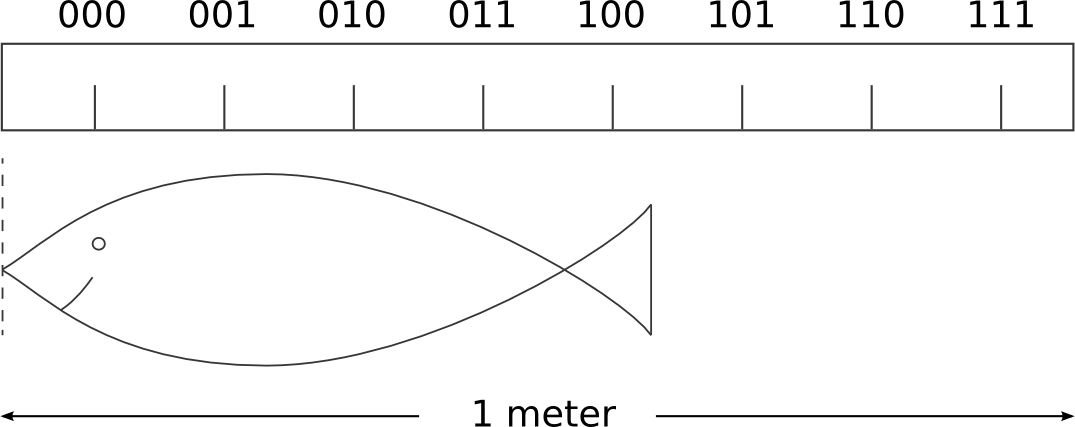
\includegraphics[width=\FigWidth\textwidth]{fish.png}
\caption{Measuring our catch with a digital ruler.}
\label{f:fish}
\end{figure}

Remember, that our digital ruler can only report a 3-bit number.  From the illustration we might anticipate that the ruler would report the binary number $100$ since that is closest to the actual length of our fish.  However, since most of our friends are engineers, they will expect our fishing story to have engineering units.  How do we convert this binary number to an actual length?

Since we know the range of our measurement (\unit[1.0]{m}) and the total number of bits (4) we can convert to a length ($L$) using a ratio
\begin{equation}
L = FSR \left(\frac{X}{2^M - 1}\right
) = (1.0 m)(4/7) = 0.57 m
\end{equation}
where $X$ is the decimal equivalent of our binary measurement ($100$).  

From the illustration it should be clear that the resolution of this measurement is fairly course.  In particular, the resolution ($Q$) can be calculated using the full sale range and the number of bits in our instrument using the relationship
\begin{equation}
Q = \frac{FSR}{2^M} = \frac{\unit[1.0]{m}}{2^3} = \unit[0.125]{m}.
\end{equation}
So, in reality we might report our measurement as \unit[0.57]{m} with a resolution of  \unit[0.125]{m}.  In other words we are saying that the length of our fish is somewhere between \unit[0.51]{m} and \unit[0.63]{m}.  So any fish with a length between \unit[0.51]{m} and \unit[0.63]{m} would generate the same report from our digital ruler - $100$.

\begin{ex}
If we had a digital ruler with twice the number of bits (6-bits instead of 3-bits) what would be the resolution of our measurement be (with engineering units)?
\end{ex}

\ifsolutions
\begin{soln}
\[
Q = \frac{FSR}{2^6} = \frac{1.0}{64} = \unit[0.0156]{m}
\]
The answer must have a number and units (m).
\end{soln}
\fi


\section{Digital Measurements in an Analog World}
\label{s:dac}
Moving on from our tall tale we are now prepared to discuss making measurements using a digital device, for instance a computer or micro-controller.  With the ubiquity of computational devices many observations we make today are done with these devices and at the foundation is the concept of an \gls{analog-to-digital converter} (ADC) or (A/D).  The details of how an ADC does it work is beyond the scope of this discussion.  What is important is to understand the conceptual idea of converting an analog signal, which can have an infinite number of values within a range, to a digital signal, which is represented by a finite number of levels.  The number of levels that this digital signal can take on is specified by the number of bit, just as our 3-bit digital meter stick from Figure~\ref{f:fish} could only report 8 individual values.  

To begin our discussion of digital measurements let's consider a simplified case where an analog voltage comes in from the outside world (from a sensor) and the ADC converts the voltage to a binary number.  As an example let's consider an ADC with the following properties:
\begin{itemize}
\item FSR = \unit[0--10]{V}
\item 8-bit resolution
\end{itemize}

The job of the ADC is to convert the incoming voltage and convert the value to a binary number that most closely represents the value as illustrated in Figure~\ref{f:adc}
\begin{figure}[hbt!]
\centering
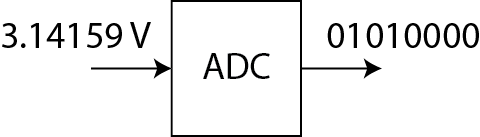
\includegraphics[width=\FigWidth\textwidth]{adc.png}
\caption{Analog-to-digital conversion: analog voltage input and binary number output.}
\label{f:adc}
\end{figure}
An important consideration of this ADC example is the resolution of the measurement, also known as the quantization error, which can be calculated using the same expression as before:
\begin{equation}
Q = \frac{FSR}{2^M} = \frac{\unit[10.0]{V}}{2^8} = \unit[39.1]{mV}.
\end{equation}
Because the ADC has 8-bits of resolution, it will report a binary number that is one of 256 possible levels.  Each level is separated by \unit[39.1]{mV} so that the total range is \unit[10.0]{V}.  If the actual input voltage is \unit[3.14159]{V} the ADC will report the closes binary level that correspond to this measurement which is $01010000$ (80 in decimal form).  So the ADC output, converted back to voltage, would be \unit[3.125]{V} $\pm$ \unit[0.0196]{V}, where \unit[0.0196]{V} is $Q/2$.  

Now if it wasn't bad enough that our 8-bit ADC has such coarse resolution, we also have to contend with the fact that the input voltage might be much smaller than the incoming range.  Consider what would happen if the actual input voltage only range between \unit[0--0.1]{V}, instead of the \unit[0--10.0]{V} range of the ADC.  In this case the ADC would only have four possible outputs corresponding to 0, 0.0391, 0.0782 and 0.1173 V.  So, in effect we would only be using 2-bits of our 8-bit ADC!

\begin{ex}
Consider an analog-to-digital converter with the following properties:
\begin{itemize}
\item FSR = $\pm$ \unit[1.0]{V}
\item 12-bit resolution
\end{itemize}
What is the resolution (in Volts) of the ADC?  If the input to the ADC was \unit[3.14]{V}, what binary number would be output by the ADC?
\end{ex}

\ifsolutions
\begin{soln}
\[ 
Q = \frac{2.0}{2^{12}} = \unit[0.0005]{V}
\]
The second part is a bit of a trick question.  Because the input is larger than the FSR, then the output would be the maximum value of the ADC - which is $2^{12}$ or 4,096.  
\end{soln}
\fi

\section{Summary}
The point of all this is the following:
\begin{itemize}
\item Digital representations of analog measurements have only finite resolution.
\item The input signal must be well matched to the ADC range to effectively use the full resolution of the ADC.  
\end{itemize}

So far we've just considered the simple idea of converting static analog measurement to a digital representation.  In the next chapter we'll consider what happens when we consider another dimension---time---in our understanding of measurement systems.  We'll also look at how to couple the ADC component with the rest of our system to make quality observations.

\section{Exercises}
\begin{ex}
Visit your favorite on-line vendor and search for a computer (PC or Mac) sound card.  Report the following specifications:
\begin{itemize}
\item Make and Model
\item Price
\item Audio input resolution (in bits)
\item Audio input range (in Volts)
\item Maximum sample rate (in Hz)
\end{itemize}
\end{ex}



\printglossary[type=\thisgls]
\glsresetall

\renewcommand{\thisgls}{model1}
\newglossaryentry{first-order model}
{
type=\thisgls,
name={first-order model},
description={A first-order, linear, time-invariant ordinary differential equation.}
}
\newglossaryentry{time constant}
{
type=\thisgls,
name={first-order model},
description={For a first-order model with a step input, the time duration from the initiation of the step to the time when the model output is 63.2\% of the way to the steady-state value.},
symbol={\ensuremath{\tau}}
}

\newglossaryentry{mathematical model}
{
type=\thisgls,
name={first-order model},
description={An equation or set of equations that behave in a similar way to a physical system under certain conditions.}
}

\newglossaryentry{step function}
{
type=\thisgls,
name={step input},
description={A mathematical function that is zero for all time less than $t=0$ and unity for all time greater than or equal to $t=1$.},
symbol={\ensuremath{\mu(t)}}
}

\newglossaryentry{step response}
{
type=\thisgls,
name={step response},
description={The output of a mathematical function, as a function of time, when a step input is given as the input or forcing function.}
}

\newglossaryentry{steady-state response}
{
type=\thisgls,
name={steady-state response},
description={The output of a mathematical model or physical system when in equilibrium.  The steady-state response is often contrasted with the transient response.}
}
\newglossaryentry{superposition}
{
type=\thisgls,
name={superposition},
description={The property of linear mathematical models that states that the total response of the system caused by two (or more) inputs is the sum of the responses to each input considered independently}
}


\chapter{Dynamic Models: Part 1}\label{c:model1}
\renewcommand{\epigraphsize}{\small\itshape}
\renewcommand{\epigraphwidth}{4.25in}
\renewcommand{\epigraphrule}{0pt}
\begin{epigraphs}
\qitem{The best material model of a cat is another, or preferably the same cat.}{--- \textup{Arturo Rosenblueth and Norbert Wiener}, \\The Role of Models in Science, 1945.}
\end{epigraphs}

\section{All Models Are Wrong!}
For our purposes a \emph{model} is equivalent to a \gls{mathematical model}, an equation.  We can use to understand and design a \emph{system}, a physical system which we wish to analyze.  Over the last few hundred years people with last names like Newton, Maxwell, Euler, Lagrange  and Bernoulli have come with a variety of simple equations that describe physical processes.  The key point, that is often overlooked, is that this description is only approximate; the mathematical model and the physical system never share the same behavior.

So why do engineers spend so much time and energy learning mathematical equations and how to solve them if these models never completely capture the behavior of a physical system?  It turns out that under specific conditions, these models allow us to \emph{predict} the behavior of systems that we might want to build.  

As an example, consider the Hoover Dam, a \unit[726]{ft} tall structure constructed with over 3 million cubic yards of cement.  In designing this structure we would hope that engineers spent a large amount of time on structural models to attempt to predict if their designs would last through floods, earthquakes and any situation that might arrive.  Without any models they would be have to fall back on the build-and-test process of engineering, building a prototype dam and sitting back to see if it worked; obviously not a very safe or cost effect way to build a dam.  On the other hand, we have to imagine that the engineers included some conservative factors of safety to build the structure somewhat larger and stronger than their models predicted.  They did this because they understood that the model was only an approximation of the dam; the model was wrong, but still useful.  

So, even though models are wrong (they are always simplified approximations), they are useful for the following reasons:
\begin{itemize}
\item under certain specific conditions mathematical models can predict (approximately) the behavior of physical systems
\item analysis of the model behavior can be an efficient way to test the behavior of system designs before we go to the trouble (cost and time) to build the physical system
\item we can analyze the behavior of models in situations that would be hard or impossible to create in the physical system
\item the model analysis enables us to understand the system and build intuition about how a system behaves 
\end{itemize}

\section{First-Order Model}
Our \gls{first-order model}---a first-order, linear, ordinary differential equation---is 
\begin{equation}
\label{e:first}
\frac{dy(t)}{dt} + \frac{1}{\tau}y(t) = f(t),
\end{equation}
where $f(t)$ is the input (forcing function), $y(t)$ is the output (response function) and $\tau$ is the time constant.  That's it; there is really nothing more to say.  

But of course we do have much more to say.  I want to start by emphasizing that this model is just as wrong as the rest of them (but it can be very useful).  There are two reasons that this model is useful:
\begin{enumerate}
\item The time-response of this model is sufficiently similar to that of many physical systems to allow us to use this fictitious model (equation) to predict how an actual system might behave.
\item We know (or we will know shortly) how to solve this equation to calculate the output of the model in response to a variety of inputs.
\end{enumerate}








\subsection{An Example}
One example of a physical system that can be approximated by our first-order model is an automobile.  Let's consider how the speed of an automobile (the output) responds to changes in the gas petal (the input) as it moves in a constant direction.  The sketch if Figure~\ref{f:massd} illustrates this simplification of a complex physical system. 
\begin{figure}[hbt!]
\centering
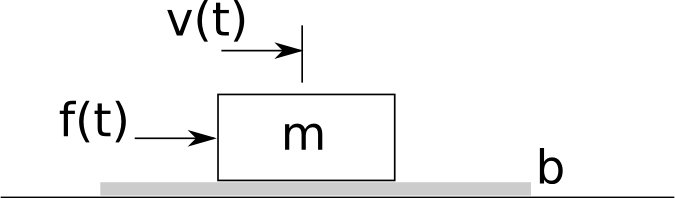
\includegraphics[width=\FigWidth\textwidth]{mass_damper.png}
\caption{Sketch of a simplified automobile model.  The point mass ($m$) moves to the right at a velocity ($v(t)$.  The input is a force ($f(t)$) and the drag force ($b (v(t))$ resists the motion. }
\label{f:massd}
\end{figure}
Based on this sketch we can do things like draw a free-body-diagram and apply Newtonian principles to arrive at an equation of motion.  We might also make an ambitious simplifying assumption that the drag force that resists the motion of the mass is linearly related to the velocity, i.e., $f_{\mathrm{drag}}=b(v(t))$.  Then we could come up with an equation of motion
\begin{equation}
\label{e:car}
m\left(\dot{v}(t)\right) + b(v(t)) = f(t)
\end{equation}
where $m$ is the mass of the car, $v(t)$ is the speed, $\dot{v}(t)$ is the acceleration, $b$ is the coefficient of linear drag and $f(t)$ is the input force.  This equation of motion is our mathematical model
This equation has the same form (a first-order, linear, ordinary differential equation) as our first-order model~(\ref{e:first}).

This is meant to be an example of a model that is obviously wrong.  A physical automobile is a complex system with many, many degrees of freedom.  Our simplified model~(\ref{e:car}) is meant to do just one thing, allow us to predict how, in general, the speed of a car responds to changes in the throttle input.


\section{Step Response}\label{s:firststep}
One useful aspect of our first-order model~(\ref{e:first}) is that the solution to this differential equation is well known for a variety of input functions.  A particularly interesting input function is the \gls{step function} ($\mu(t)$) defined as
\begin{equation}
\label{e:step}
\mu(t)= \left\{ 
\begin{array}{cl}
0 & \, \mathrm{for}\, t < 0 \,\,\,\\
1 & \, \mathrm{for}\, t \geq 0
\end{array} \right.
.
\end{equation}
This function ($\mu(t)$) is also known as the \emph{unit} step function because the amplitude of the step is 1.0.
Figure~\ref{f:step} illustrates how the value of $\mu(t)$ is zero before $t=0$ and then instantaneously changes to unity.
\begin{figure}[hbt!]
\centering
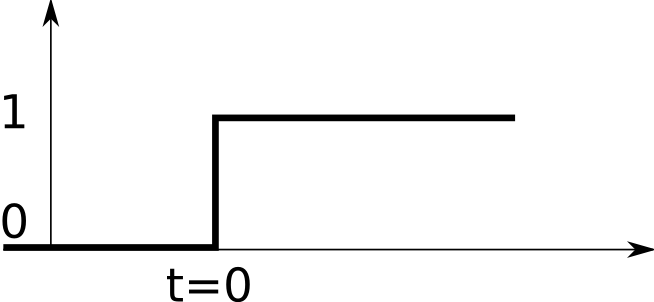
\includegraphics[width=\FigWidth\textwidth]{step.png}
\caption{Illustration of a step function $\mu(t)$.}
\label{f:step}
\end{figure}

Now consider our generic first-order model (\ref{e:first}) with a step input ($f(t)=A\mu(t)$) and an initial condition of zero ($y(0)=0$),
\begin{equation}
\label{e:firststepinput}
\frac{dy(t)}{dt} + \frac{1}{\tau}y(t) = A\mu(t).
\end{equation}
(You should notice that the input function ($f(t)$) is a step input with an amplitude of $A$.)
The \gls{step response} is the solution to this ordinary differential equation which is
\begin{equation}\label{e:stepresp}
y(t) = A\tau\left(1-e^{-t/\tau}\right)
\end{equation}
for $t>0$.  Notice that there are two key parameters of our model step response: the time constant ($\tau$) and the amplitude of the step input ($A$).

\begin{figure}[hbt]
\centering
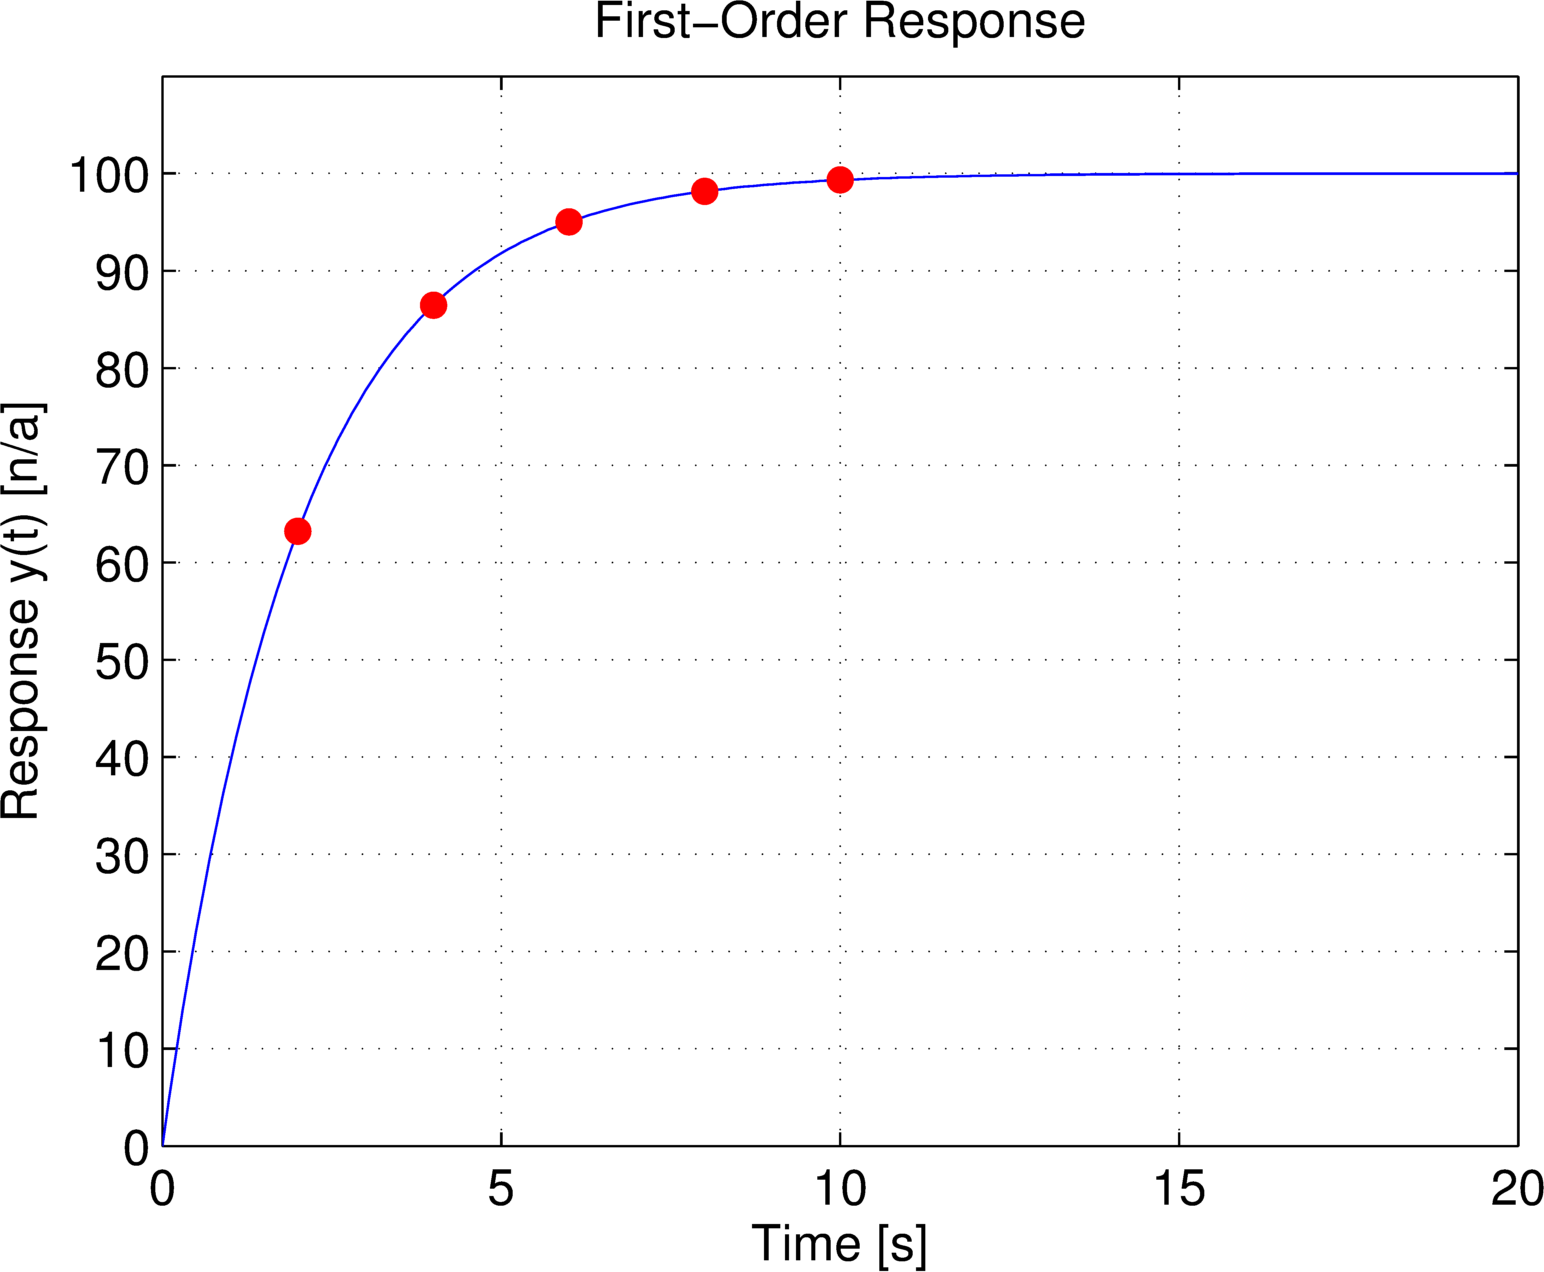
\includegraphics[width=\textwidth]{first_step.png}
\caption{Graph of the step response (\ref{e:stepresp}) with $\tau=\unit[2]{s}$ and $A=50$.  The red dot markers indicate the value of the solution at $t=[\tau,2\tau,3\tau,4\tau,5\tau]$. }
\label{f:firststep}
\end{figure}


\lstinputlisting[style=myMatStyle,
caption={Script for first-order response: first\_order\_response.m},
label={l:firstresp}]
{../code/first_order_response.m}


This solution (\ref{e:stepresp} is graphed in Figure~\ref{f:firststep} using the MATLAB script in Listing~\ref{l:firstresp}. This time response to a step input (or step response for short) has a characteristic shape as it rises and approaches the \gls{steady-state response} exponentially.  One important aspect of the response is that it approaches a new constant value, the steady-state response.  A simple way to find the steady state value is to set $\dot{y}(t)=0$ in (\ref{e:first}).  Since we are looking for the ``steady-state'' value we can anticipate that all rates of change (derivatives) will be zero.  Now the steady-state value ($y_{\mathrm{ss}}$) is 
\begin{equation}\label{e:ss}
y_{\mathrm{ss}} = \tau A.
\end{equation}

Another important characteristic of this model is that the response ($y(t)$) moves exponentially from the initial value to the steady state value.  This response is characterized by the the \gls{time constant} ($\tau$).  If we evaluate time response (\ref{e:stepresp}) at $t=\tau$ we find that
\[
y(t=\tau) = A \tau (0.632) = 0.632 (y_{\mathrm{ss}})
\]
which means that after one time constant has passed the response is 63.2\% of the way from the initial value to the steady state value.  Take a look at Figure~\ref{f:firststep} to make sure that we did the math correctly!

\subsection{Car Example---Step Response}
Now that we've discussed the time response of our first-order model let's see how this applies to our automobile model.  We can rearrange the mathematical model (\ref{e:car}) so that it looks more like our generic model (\ref{e:first}) which results in the expression
\begin{equation}\label{e:car2}
\dot{v}(t) + \frac{1}{m/b}(v(t)) = \frac{F}{m}\mu(t)
\end{equation}
which highlights that the time constant is $\tau=m/b$ and that the steady state speed is $v_{\mathrm{ss}}=F/b$.  Take a moment to think about this.  It means that the larger the mass of our car, the slower the acceleration (because the time constant is larger).  You might also notice that the mass has no effect on the steady state speed; our model says that a heavy ``car'' will reach the same final speed as a light car, it will just get there slower.  Finally we might notice that the more drag in our model, the slower our ``car'' will go for the same input. Listing~\ref{l:carresp} illustrates how we might use MATLAB to graph the solution for specific numerical values.

\lstinputlisting[style=myMatStyle,
caption={Script for first-order response of our car example: firstorder\_car\_ex.m},
label={l:carresp}]
{../code/firstorder_car_ex.m}

\begin{ex}
The step function in (\ref{e:step}) could be more precisely called the ``unit step function'' because it has an amplitude of 1.  Write an equation (similar to (\ref{e:step})) and sketch a graph (similar to Figure~\ref{f:step}) for the more general step function input $f(t) = A(\mu(t-t_o))$.
\end{ex}

\begin{ex}
We justified (\ref{e:ss}) by starting with the model (\ref{e:first}).  Another way to calculate the steady state response is to evaluate the solution (\ref{e:stepresp}) as $t \to \infty$.  Show that using this method yields the same result.
\end{ex}

\begin{ex}
We showed that the response of a first-order model to a step function input has an exponential increase characterized by the time constant.  Furthermore we showed that after a duration of one time constant beyond the rise in the step input the output will be 63.2\% of the way to its steady state value.  Figure~\ref{f:firststep} illustrates the value of the response at  $t=[\tau,2\tau,3\tau,4\tau,5\tau]$.  Evaluate \ref{e:stepresp} for these values of time and report the results in a two column table where the first column is the ratio $t/\tau$ and the second column is the ratio $y(t)/y_{\mathrm{ss}}$.
\end{ex}

\begin{ex}
\label{ex:carstep}
Consider the step response to our car model (\ref{e:car2}) with the following parameters: mass = \unit[800]{kg}, drag coefficient = \unitfrac[225]{Ns}{m}, step input amplitude = \unit[15,000]{N}.  Using MATLAB, create a graph similar to Figure~\ref{f:firststep} to illustrate the step response of our ``car''.  Annotate the graph to show the time constant and the steady state speed.  Also, make sure to use appropriate units for each axis.
\end{ex}

\begin{ex}
Consider the step response to our car model (\ref{e:car2}) with the parameters given in Exercise~\ref{ex:carstep}
\begin{itemize}
\item What is the minimum step input amplitude ($F_{\mathrm{min}}$) that would cause our ``car'' to go from \unit[0--60]{mph}?
\item Based on this minimum step input amplitude, how long does it take for the ``car'' to go from \unit[0--60]{mph}? (Hint: the answer to this question can be a number or a sentence!)
\item If we double $F_{\mathrm{min}}$
 \begin{itemize}
 \item How long does it take for the ``car'' to go from \unit[0--60]{mph}?
 \item What is the new top speed (in mph)?
 \item How long does it take for the ``car'' to achieve this new top speed?
 \end{itemize}
\end{itemize}
\end{ex}

\ifsolutions
\begin{soln}
Here is a solution.
\begin{itemize}
\item The steady-state value is $V_{ss}=F/b$ and \unit[60]{mph} is approximately \unitfrac[27]{m}{s}.  Since $b=\unitfrac[225]{Ns}{m}$, $F_{min}=\unit[6075]{N}$.
\item Interestingly the car never truly gets all the way to the final steady-state value!  After five time constants ($t=5\tau$=\unit[25]{s}) the car is 99\% of the way to \unit[60]{mph}
\item If we double this input force...
\begin{itemize}
\item The car takes about \unit[4]{s} to get to \unit{60}{mph} (\unitfrac[27]{m}{s}).
\item The new top speed is double of the original top speed---\unit[120]{mph}.  This is because the system is linear!
\item Again, it never really gets there.  It gets 99\% of the way there after five time constants: $\tau=m/b=\unit[3.5]{s}$ so $5\tau=\unit[17.8]{s}$.
\end{itemize}
\end{itemize}
\end{soln}
\fi


\section{Free Response}
Another useful time response of our first-order model is the response with no input ($f(t)=0$) and an initial condition ($y(0)=y_o$).  The solution to (\ref{e:first}) under these conditions is 
\begin{equation}\label{e:firstfree}
y(t) = y_o \, e^{-t/\tau}
\end{equation}
for $t>0$. Figure~\ref{f:firstfree} illustrates this free response.  Just as before the time constant is the key factor that determines the characteristic of the response.  Again, at $t=\tau$ the output has fallen by 63.2\%.
\begin{figure}[hbt]
\centering
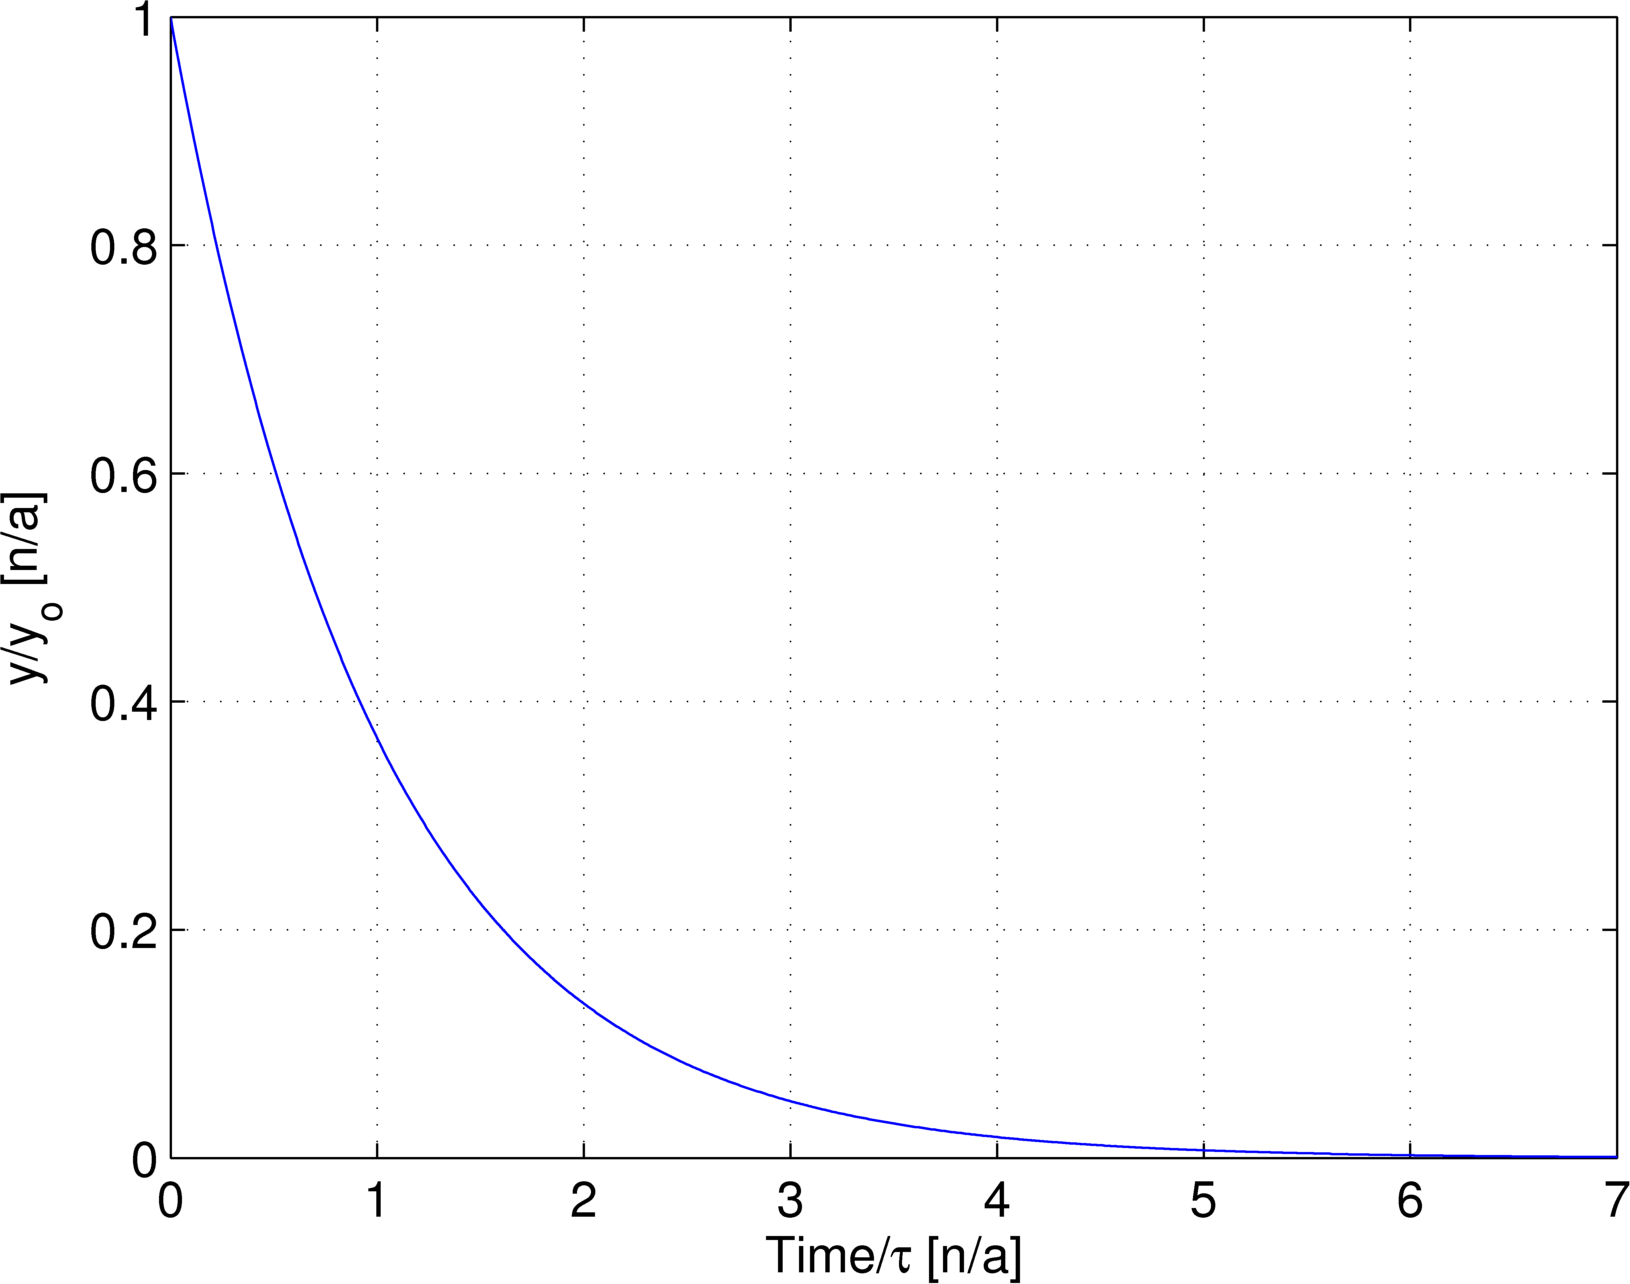
\includegraphics[width=\FigWidth\textwidth]{firstfree.png}
\caption{Graph of the free response (\ref{e:firstfree}).  Notice that the $x$ and $y$ axes have been normalized so that the output is the ratio of the response and the initial condition and the time is the ratio of time and the time constant.}
\label{f:firstfree}
\end{figure}

\begin{ex}
Using our automobile model (\ref{e:car}), write an expression for the free response of this model with appropriate physical parameters.  Create a graph of the free response with the initial condition $v(0)=\unit[60]{mph}$. For the x-axis of the graph use the units mph and for the y-axis of the graph use the units seconds.
\end{ex}



\section{Superposition---Step Response with Non-Zero Initial Condition}
One the characteristics that make linear system such as our first-order model useful is the principle of \gls{superposition} which allows determine the solution to a linear model by adding together multiple solutions.  As an example, suppose there are two input functions, $f_1(t)$ and $f_2(t)$, and that the corresponding solutions are $y_1(t)$ and $y_2(t)$.  If we want to know the response of the system to both inputs, $f(t)=f_1(t)+f_2(t)$, we can simply add the two solutions, $y(t)=y_1(t)+y_2(t)$. 

This principle simplifies the task of finding the response to our first-order model when there are both initial conditions and a forcing function.  Armed with superposition principle we can determine the step response (the solution to (\ref{e:first}) with the input $f(t)=A\mu(t)$) of our first-order model when there is a non-zero initial condition ($y(0)=y_o$) by simply adding our two previous solutions, the step response with zero initial condition and the free response with no forcing function:
\begin{equation}
y(t) = y_o \, e^{-t/\tau} + A\tau\left(1-e^{-t/\tau}\right).
\end{equation}

Another handy aspect of superposition is the scaling property.  This means that if we scale (multiply) the input by a factor ($a$) then the output is simply the response to the original input scaled (multiplied) by the same factor.  As an example, consider our first-order car model (\ref{e:car}) where the input is a force ($f(t)$).  If we know that a force of \unit[1,000]{N} results in a steady state speed of \unit[25]{mph} then superposition tells us that a force of \unit[2,000]{N} will result in a final speed of \unit[50]{mph}.

\begin{ex}
Consider our first-order car model discussed above where a \unit[1,000]{N} input yields a steady state speed of \unit[25]{mph}.  Furthermore, we know that the time constant of this system is \unit[2]{s}.  Again we double the input to from \unit[1,000]{N} to  \unit[2,000]{N}. What is the time constant of the response with the doubled input?

Hint: This might be considered a 'trick' question.
\end{ex}


\section{Thermometer Example}

Our first-order model can be used to describe the response of a temperature sensor to changes in the ambient environment.  This is analogous to our ``car'' model in that the temperature sensor has thermal inertia (analogous to the mass of our ``car'') and thermal resistance (analogous to the drag of our ``car'').  

\subsection{Mathematical Model}
Suppose we have a bulb thermometer that is at equilibrium the instant before it is plunged into boiling water.  The measured temperature will not instantly move to \unit[100]{$^{\circ}$C}, but instead the temperature of the device ($T(t)$) will move toward the new equilibrium over time.  The speed of that response is determined by the inertia and resistance of the system.

Figure~\ref{f:therm} illustrates how we might analyze this system.  Newton's law of cooling says that ``the rate of heat loss of a body is proportional to the difference in temperatures between the body and the surroundings'', or, stated mathematically,
\begin{equation}
\dot{Q}=hA (T_f(t)-T(t))
\end{equation}
where $\dot{Q}$ is the rate of heat transfer, $h$ is the heat transfer coefficient, $A$ is the surface area of the thermometer, $T_f(t)$ is temperature of the surroundings and $T(t)$ is the temperature of the thermometer.  Furthermore the thermal energy in the thermometer mass is $Q=C(T(t))$ where $C$ is the total heat capacity (the product of the mass ($m$) and the specific heat capacity of the material ($c_p$)).  Putting this together we can come up with a first-order model for a thermometer
\begin{equation}
\label{e:therm}
\dot{T}(t)= \frac{hA}{C}(T_f(t)-T(t)).
\end{equation}

\begin{figure}[hbt]
\centering
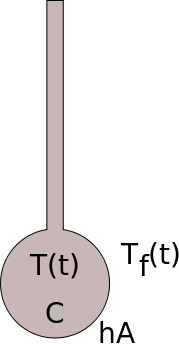
\includegraphics[width=0.20\textwidth]{thermometer.png}
\caption{Illustration of a simple model of the response of a thermometer.}
\label{f:therm}
\end{figure}

\begin{ex}
Using (\ref{e:therm}) rearrange the terms so that the expression has the same form as our canonical first-order model (\ref{e:first}).    What is the input to our model?  What is the output of our model?  What is the time constant of this model?  What is the steady-state temperature predicted by this model?
\end{ex}

\ifsolutions
\begin{soln}
\[ 
\dot{T}(t)+\frac{hA}{C}(T(t)) = \frac{hA}{C} (T_f(t)) 
\]
where $\tau = \frac{C}{hA}$.
\begin{itemize}
\item The input is the temperature of the surrouding fluid---$T_f(t)$.
\item The output is the temperature of the sensor---$T(t)$.
\item The time constant is $\tau = \frac{C}{hA}$
\item The steady state temperature is $T_{ss}=T_f$.
\end{itemize}
\end{soln}
\fi


\printglossary[type=\thisgls]
\glsresetall

\renewcommand{\thisgls}{measure}

\newglossaryentry{data acquisition system}
{type=\thisgls,
name={data acquisition system},
description={Assembly of sensors, signal conditioning, digital-to-analog converter and a display or storage device for collecting physical measurements as digital records.},
symbol={DAS or DAQ}
}

\newglossaryentry{transducer}
{type=\thisgls,
name=transducer,
description={A device for converting on type of energy to another type of energy.  Examples include both sensors and actuators.}
}
\newglossaryentry{ratiometric}
{type=\thisgls,
name=ratiometric,
description={Refers to the situation where the output (voltage) is a ratio of the supply or excitation voltage.}
}
\newglossaryentry{excitation voltage}
{type=\thisgls,
name=excitation voltage,
description={The constant voltage supplied to power a sensor, typically a strain gage or Wheatstone bridge.}
}
\newglossaryentry{full scale voltage range}
{type=\thisgls,
name={full scale voltage range},
description={The specified input voltage range to an ADC.  The range can be bipolar (both positive and negative, e.g., $E_{\mathrm{FSR}}=\pm\unit[1.0]{V}$) or unipolar (only positive, e.g.,  $E_{\mathrm{FSR}}=\unit[0--1.0]{V}$.)}
symbol={\ensuremath{E_{\mathrm{FSR}}}}
}
\newglossaryentry{quantization error}
{type=\thisgls,
name={quantization error},
description={the difference between the actual analog input to a analog-to-digital converter and the reported digital (or quantized) value.},
symbol={\ensuremath{\pm Q/2}}
}
\newglossaryentry{differential input}
{type=\thisgls,
name={differential input},
description={the input configuration of an A/D where the output measures the difference between two voltages (+ and -) that are independent of electrical ground.}
}
\newglossaryentry{single-ended input}
{type=\thisgls,
name={single-ended input},
description={the input configuration of an A/D where the output measures the voltage of a single voltage (+) relative to a common electrical ground (GND).}
}
\newglossaryentry{sampling period}
{type=\thisgls,
name={sampling period},
description={For an A/D, the duration in time between sampling events in units of time, e.g, seconds.},
symbol={\ensuremath{dt}}
}

\newglossaryentry{sampling frequency}
{type=\thisgls,
name={sampling frequency},
description={For an A/D, the frequency of sampling events which is the reciprocal of the sampling period, typically in units of Hz.},
symbol={\ensuremath{f_s}}
}
\newglossaryentry{Nyquist frequency}
{type=\thisgls,
name={Nyquist frequency},
description={For the output of an A/D the Nyquist frequency is the highest frequency of the signal that can be observed in the digital version of the signal.  Because the Nyquist frequency is half of the sampling frequency, it is important to sample sufficiently fast to capture all the dynamics in the input.}
}

\newglossaryentry{aliasing}
{type=\thisgls,
name={aliasing},
description={The result of having energy in the input to an A/D with frequency content higher than the Nyquist frequency.  These higher frequencies are aliased into the digital representation to cause errors.}
}

\chapter{Data Acquisition}\label{c:daq}

\section{Data Acquisition Systems}
Figure~\ref{f:daq} illustrates a typical \gls{data acquisition system} which consists of the following components:
\begin{itemize}
\item Sensor(s): Device for converting a physical quantity into an analog signal, e.g., accelerometer, thermocouple or strain gage.
\item Signal Conditioning: Electronics for adapting sensor output to comply with the input of a DAC, e.g., filtering, Wheatstone bridge or amplification.
\item Digital-to-Analog Converter (DAC): See Section~\ref{s:dac}.
\item Destinations: Digital display (e.g., 2D graph) or archive (e.g., log file).
\end{itemize}

\begin{figure}[hbt!]
\centering
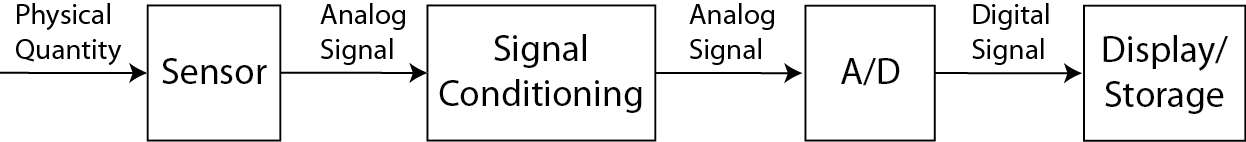
\includegraphics[width=\FigWidth\textwidth]{daq.png}
\caption{Simple data acquisition system diagram.}
\label{f:daq}
\end{figure}

In this chapter we'll work through each of the subsystems in Figure~\ref{f:daq} to discuss how they operate together to create a system for making digital measurements.

\section{Sensors}
A \gls{transducer} is a device that converts one type of energy into another type of energy.  A sensor is a transducer, but not all transducers are sensors.  (The opposite of a sensor is an actuator).  Here are some examples:
\begin{itemize}
\item A microphone is a transducer that converts acoustic energy (sound pressure) to electrical energy (voltage). A microphone is a sensor.
\item A speaker is a transducer that converts electrical energy to acoustic energy.  A speaker is an actuator.
\item An accelerometer is a transducer that converts mechanical energy (vibration) to electrical energy (voltage).  An accelerometer is a sensor.
\item An electric motor is a transducer that converts electrical energy to mechanical energy (rotation).  An electric motor is an actuator.
\item A thermocouple is a transducer that converts thermal energy (temperature) to electrical energy (voltage).  A thermocouple is a sensor.
\item A heating coil is a transducer that converts electrical energy to thermal energy.  A heating coil is an actuator.
\end{itemize}

\begin{ex}
Following the pattern in the list above, list two more transducers that are sensors and two more transducers that are actuators.
\end{ex}


There are many, many types of sensors.  For just about everything we can imagine wanting to measure there is a device that will convert the physical parameter to an electrical signal that we can use for data aquisition.  For our purposes we will focus on sensors that measure mechanical quantities (motion, strain, temperature, etc.) by producing an electrical output.  The next step is converting that electrical output into a form that our D/A can accept.  

\subsection{Sensitivity}
The sensitivity of a sensor is the parameter of the sensor that describes the transduction.  In simple cases the sensitivity of a sensor is given as a ratio between the output (typically voltage) and the physical input.  For example, the ADXL 335 accelerometer has a typical sensitivity of \unitfrac[300]{mV}{g} which means that for an input acceleration of \unit[1.0]{g} the sensor output will be \unit[300]{mV}.
\begin{ex}\label{ex:asens}
Suppose we are going to use an ADXL 335 accelerometer to measure the acceleration of a radio-controlled car.  We know that the car has a maximum forward acceleration of \unitfrac[2.5]{m}{s$^2$}.  What is the maximum output voltage we could expect from the accelerometer?
\end{ex}
\begin{ex}
A Type K thermocouple is a common sensor for measuring temperature, and the typical sensitivity for such a device is \unitfrac[41]{$\mu$V}{$^{\circ}$C}.  What output voltage could we expect if we were using this device to measure the temperature of boiling water (at sea-level)?
\end{ex}

A complication that can arise is when the sensitivity of a sensor is not a constant.  This can happen if there is a non-linear relationship between the physical parameter and the output.  In this case we may have to use a mathematical relation (i.e., a formula, hopefully supplied by the sensor datasheet) to convert the output signal (voltage) to the physical measurement.  Another situation is when the output depends on the supplied voltage, which is called a \gls{ratiometric} sensitivity.  In fact, I oversimplified the ADXL 335 sensitivity.  This sensor requires a supply voltage, sometimes referred to as the \gls{excitation voltage}, to power the sensor.  The typical supply voltage is \unit[3.0]{V}, but the value can range between \unit[1.8--3.6]{V}.  The sensitivity is directly proportional to this supply voltage, so with a supply of \unit[1.8]{V} we can expect a sensitivity of \unitfrac[180]{mV}{g}.  

Another common example of a ratiometric sensitivity is a load cell.  As its name implies, a load cell is a sensor that reports a load (tension or compression) as a voltage.  A common type of load cell is S-Beam load cell that uses a configuration of strain gages to measure the strain in a mechanical beam.  The beam is calibrated so that the relationship between the strain and the applied force is known.  The sensitivity of this type of sensor is specified in a confusing manner.  For example, a typical device will come in a range of load capacities, say \unit[25-10,000]{lb}.  For this family of devices the sensitivity might be quoted as \unitfrac[3]{mV}{V}.  What on earth does this mean you ask?  Well, it means that at the maximum load, the output voltage is \unit[3]{mV} multiplied by the excitation voltage.  They typical excitation voltage of this particular device is \unit[10]{V}.  So, if we have a load cell rated at \unit[100]{lb} and we apply the recommended excitation of \unit[10]{V}, the sensitivity is \unitfrac[0.3]{mV}{lb}.  In other words, we can find the sensitivity (\unitfrac[S]{mV}{lb}) as
\begin{equation}\label{e:sens}
\unitfrac[S]{[mV}{lb]} = \frac{(\unitfrac[O]{[mV}{V]})(\unit[E]{[V]})}{\unit[L_{max}]{[lb]}}
\end{equation}
where \unitfrac[O]{[mV}{V]} is the ratiometric output of the load cell, \unit[E]{[V]} is the excitation voltage and \unit[L$_{\mathrm{max}}$]{[lb]} is the maximum load capacity for the device.
\begin{ex}
Suppose we want to use two AA alkaline batteries to power our ADXL 335 accelerometer.  What sensitivity could we expect with this arrangement?
\end{ex}
\begin{ex}
Consider that we are using a thin-beam load cell (Omega LCL Series) with a maximum load capacity of \unit[1]{lb}.  The rated output of the load cell is \unitfrac[2]{mV}{V} and the recommended excitation is \unit[5]{V}.  
\begin{itemize}
\item What is the sensitivity of the load cell in \unitfrac[]{mV}{lb}?
\item What is the maximum voltage we could expect when the load cell is at its maximum capacity load?
\item What is the voltage we could expect if we apply a \unit[0.25]{lb} load?
\end{itemize}
\end{ex}

\ifsolutions
\begin{soln}
The sensitivity is calculated using (\ref{e:sens}).
\[
\unitfrac[S]{[mV}{lb]} = \frac{(\unitfrac[2.0]{[mV}{V]})(\unit[5.0]{[V]})}{\unit[1.0]{[lb]}} = \unitfrac[10.0]{mV}{lb}
\]

The maximum voltage is the product of the maximum load and the sensitivity.
\[
V_{max} = \unitfrac[10]{mV}{lb} (\unit[1]{lb}) = \unit[10]{mV}
\]

Again, this is the product of the senitivity and the load.
\[
V_{max} = \unitfrac[10]{mV}{lb} (\unit[0.25]{lb}) = \unit[2.5]{mV}
\]
\end{soln}
\fi


\section{Signal Conditioning}
Sensors often have an output that is inconvenient to use with digital-to-analog converters.  As we alluded to in Chapter~\ref{c:measure}, digital-to-analog converters typically take a voltage as input and it is important that we use the full range of the voltage that the D/A will accept (e.g., \unit[0--10]{V}).  

Consider the case of a strain gage, illustrated in Figure~\ref{f:condition}.  The specifics will be discussed in more detail later, but for now it will suffice to say that a strain gage is a sensor that converts a strain (a change in length) to a change in electrical resistance.  This is great, but how do we plug that into our D/A which wants a voltage between \unit[0--10]{V}?  It turns out that Sir Charles Wheatstone found a solution to this problem in an elegant circuit that is now called the Wheatstone bridge.  This circuit converts the change in resistance to a very small voltage, say \unit[0--10]{mV}.  Now we have another problem, our D/A wants a much larger voltage that the \unit[10]{mV} coming from the Wheatstone bridge.  Perhaps we could add an amplifier that will multiply the output of the bridge by a gain of 1,000 so that we now have a  voltage that is suitable for the D/A.  

\begin{figure}[hbt!]
\centering
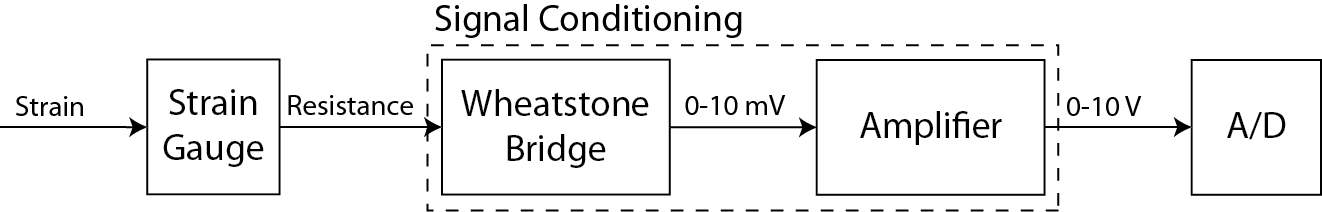
\includegraphics[width=\FigWidth\textwidth]{condition.png}
\caption{Signal conditioning example.  In the case of the strain gage, a Wheatstone bridge and amplifier are used to condition the signal before it is passed to the analog-to-digital converter.}
\label{f:condition}
\end{figure}

For our purposes two general types of signal conditioning will play an important roll in designing our measurement systems, amplification and anti-aliasing.  For now we'll discuss amplification and we'll save the topic of anti-aliasing for Section~\ref{s:alias}.

\subsection{Amplifiers}
The roll of an amplifier in our signal conditioning system is to scale the electrical output of a sensor (typically voltage) to match the input range of the analog-to-digital converter.  As we discussed in Section~\ref{s:dac}, in order to take full advantage of the resolution of our A/D, the signal range must be approximately equivalent to the input range of our A/D.  In theory (always a dangerous first two words), the function of an amplifier is to provide a multiplicative gain in the signal path, i.e., 
\[
V_{out} = K\left(V_{in}\right)
\]
where $V_{in}$ is the input to the amplifier, $V_{out}$ is the amplifier output and $K$ is the amplifier gain. 

\begin{ex}
Building on Exercise~\ref{ex:asens} consider that we want to interface our ADXL 335 into an A/D that has a range of \unit[0--10]{V} and 12-bits of resolution.  
\begin{itemize}
\item If we did not use any amplification, what would be the effective resolution (in bits) of our A/D?  (Hint: See Section~\ref{s:dac}.)
\item What amplifier gain would you suggest so that we could use the full resolution of the A/D?
\end{itemize}
\end{ex}

\section{Analog-to-Digital Conversion}
We started our discussion of A/D devices in Section~\ref{s:dac}.  Here we'll add some detail to our description of these devices.  Again, we'll focus on \emph{what} these devices do and leave the specifics of \emph{how} they do this (successive-approximation, sigma-delta, etc.) to another book.
\subsection{Range and Resolution}
Recall that the function of an ADC is to convert an voltage input (analog) to a binary number (digital).  The \gls{full scale voltage range} ($E_{\mathrm{FSR}}$) is the span of voltage inputs that the A/D will accept.  This range comes in two flavors: bilateral or unilateral.  A bilateral input range is typically symmetric about \unit[0]{V} while a unilateral input can only accept positive voltage values.  For example,
\begin{itemize}
\item Bilateral Input Range: $\pm$\unit[10]{V}
\item Unilateral Input Range: \unit[0--10]{V}
\end{itemize}
In either case the full scale range is simply $E_{\mathrm{FSR}}=V_{\mathrm{max}}-V_{\mathrm{min}}$ where the maximum input voltage is $V_{\mathrm{max}}$ and the minimum input voltage is $V_{\mathrm{min}}$.  
\begin{ex}
For the bilateral and unilateral examples above what is $E_{\mathrm{FSR}}$ for each case?
\end{ex}

Any voltage within the input range is converted to a binary value.  The length of this binary number is specified by the number of bits ($M$) inherent to the A/D, e.g., 12-bits.  The length of the binary representation determines the finite number of voltage levels that can be represented (see Section~\ref{s:dac}), so the ratio of the full voltage range to the number of levels that we can use in that range determines the resolution $Q$ (in Volts) of the A/D,
\begin{equation}
\label{e:q}
Q = \frac{E_{\mathrm{FSR}}}{2^M}.
\end{equation}
You might notice that the resolution of an A/D is often referred to as either the number of bits used in the conversion ($M$) or the resolution in volts ($Q$).  This is somewhat sloppy nomenclature, but common. 

A related concept is \myglssym{quantization error} which is another way of describing the finite resolution of converting a continuous analog value to a discrete digital value.  As we discussed in Section~\ref{s:dac}, the A/D will associate the incoming voltage level (which can assume an infinite number of possible values) with the binary representation (which can only assume one of $2^M$ possible values) that is nearest that actual value.  Based on this nearest-neighbor concept the error between the actual incoming analog voltage and the reported digital value will be $\pm Q/2$, the quantization error.


\begin{ex}
An alternative to (\ref{e:q}) is to express the resolution as 
\[
Q = \frac{E_{\mathrm{FSR}}}{2^M-1}.
\]
\begin{itemize}
\item Can you explain why this might be more correct?  Try drawing a picture of a 1-bit or 2-bit scenario to understand why we might actually only have $2^M-1$ levels in our A/D.
\item Given that typical A/D hardware has more than 10-bits, and as much as 24-bits, of resolution, is the difference between these alternatives significant?  Why or why not?
\end{itemize}
\end{ex}

\ifsolutions
\begin{soln}

There are many answers to this.  The point is that the student think about what is going on here.
\begin{itemize}
\item In general, for an $M$-bit A/D there are $2^M$ possible outputs.  However, the distance between each level is $E_{FSR}/(2^M-1)$ which is more correctly associated with the resolution of the A/D
\item For any reasonably large number of bits there the is a negligible difference between these expressions.  For example, $2^{24}=16,777,216$ and $2^{24}-1=16,777,215$.  The point is that either expression is sufficient.
\end{itemize}
\end{soln}
\fi

\subsection{Differential Versus Single-Ended}
When connecting a voltage input to an A/D there are two important options: differential or single-ended input. \Gls{single-ended input} consists of a common ground (GND) that is shared between all the inputs to the A/D.  The A/D output is based on the voltage measured between the signal input (+) and ground.  In contrast \gls{differential input} consists of two voltage inputs, high (+) and low (-), which may or may not be referenced to a common GND potential.  The A/D output is then based on the voltage difference (hence differential) between the signal high and signal low potentials.  Here are some advantages of each approach:
\begin{itemize}
\item Single-ended inputs are simpler to implement
\item Single-ended inputs use the full number of channels in the A/D device. For example, a device advertised to have ``16 inputs'' will actually have 16 single-ended inputs, but only 8 differential inputs.
\item Single-ended inputs are lower in cost
\item Differential inputs are less susceptible to noise (electromagnetic or radio-frequency interference).  This is particularly important for sensors that produce very small signals, e.g., strain gages, thermocouples, load cells, etc.
\item Differential inputs can be applied in cases (such as Wheatstone bridge outputs) where there is no true connection to a common ground.
\end{itemize}

\subsection{Sampling}
So far we have been concerned with the resolution of a digital measurement in terms of the finite levels, typically of voltage, that an ADC can use to represent the analog input---the y-axis in Figure~\ref{f:sample}.  In this section we'll discuss the ramifications of the fact that the ADC operates at a finite \gls{sampling period} ($dt$), the output of the ADC changes only at discrete times.  Therefore, an ADC has finite resolution in both amplitude (i.e., voltage) and time, illustrated by the fact that the individual samples in Figure~\ref{f:sample} are discrete points in the x and y axes.
\begin{figure}[hbt!]
\centering
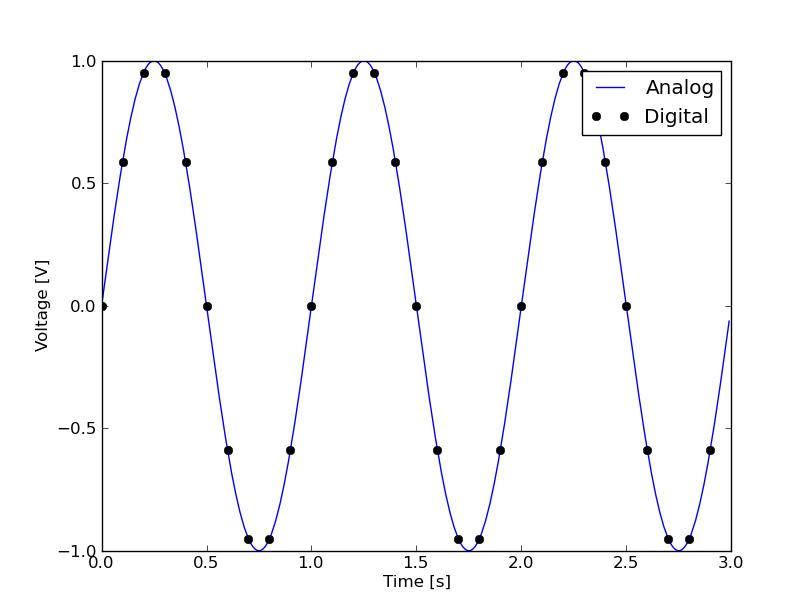
\includegraphics[width=\FigWidth\textwidth]{sample.png}
\caption{Illustration of a sampled signal.  The analog signal ($y(t)=\sin{\omega t}$) is represented by a continuous curve with an infinite set of values in both time (x-axis) and amplitude (y-axis).  The A/D converts this signal discrete samples at a finite set of time and amplitude values.}
\label{f:sample}
\end{figure}

The typical function of an A/D is to regularly sample the input voltage level and record these samples as digital numbers.  The speed at which this happens is specified by the sampling rate, or equivalently the \gls{sampling frequency} ($f_s$) where \unit[$f_s=dt$]{Hz}. (Beware, the terms ``sample rate'' or ``sampling rate'' are often used to refer to both sampling period and sampling frequency.)  The sampling is illustrated in Figure~\ref{f:sample} by the black markers; the time between each sample ($dt=\unit[0.1]{s}$) is the sampling period.


\begin{figure}[hbt!]
\centering
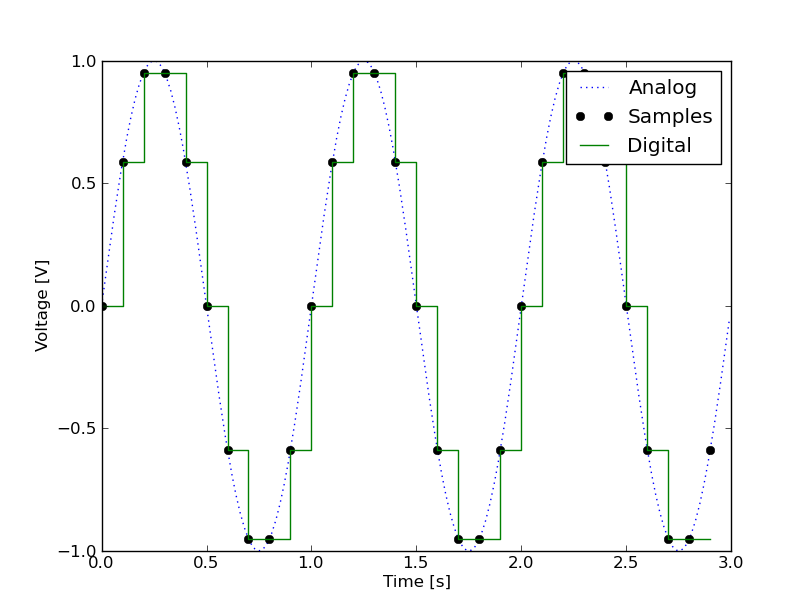
\includegraphics[width=\FigWidth\textwidth]{sample2.png}
\caption{A second illustration of the sampled signal from Figure~\ref{f:sample}. The ``Digital'' graph shows how the digital output of the A/D changes over time.  The reported value from the A/D only changes after each sampling event.}
\label{f:sample2}
\end{figure}

\begin{ex}
Consider the same analog input as illustrated in Figure~\ref{f:sample} and Figure~\ref{f:sample2}, a continuous sine wave input with a period of \unit[1.0]{s} and an amplitude of \unit[1.0]{V}.  The signal is input to a A/D with the following characteristics:
\begin{itemize} 
\item 4-bit voltage resolution
\item $E_{\mathrm{FSR}}= \pm \unit[1.0]{V}$
\item $dt = \unit[0.5]{s}$
\end{itemize}
Sketch a 2D graph (Voltage versus Time) that illustrates the analog signal and the digital samples.

\vspace{1ex}

Sketch the same 2D graph if $dt=\unit[0.33]{s}$.
\end{ex}

\subsection{How Fast to Sample?}
The sampling rate (see the warning above!) for A/D devices can vary by orders of magnitudes. Consider the contrast between two processes that we might want to measure: the rise of global temperature or the incoming voice signal from an iPhone user.  These processes evolve on very different time-scales.  To measure global temperature rise it might be sufficient to take an average measurement once per year, but a typical sampling frequency for audio input is 44,000 samples-per-second (Hz).  

\begin{ex}
Suppose we wanted to sample the global temperature at a sampling frequency of \unit{44}{kHz} using a 16-bit A/D for a year.  Estimate the size of the hard drive (in bytes) that would be necessary to store this much data.  (Hint: There are 8-bits per byte.)
\end{ex}

The sampling frequency (or period) can often be specified in software when using a ADC.  So what setting should we choose?  The simple answer is that we typically sample as fast as we can!

The longer (and hopefully more interesting) answer is that we can set a minimum necessary sampling frequency based on the characteristics of the input signal.  Let's start with our audio (iPhone) example.  The key thing you need to know is that the typical range of human hearing is from \unit[20--20,000]{Hz}.  So we'll need to sample fast enough that our digital representation (the output of the ADC) can represent this complete frequency range.  It turns out that if we collect samples at \emph{twice} the maximum frequency of interest, then we will be able to represent the analog signal with our digital representation, i.e.,
\[
f_s \geq 2\left(f_{\mathrm{max}}\right)
\]
where $f_{\mathrm{max}}$ is the \gls{Nyquist frequency}, the maximum frequency of interest in the analog signal we are trying to measure.  The Nyquist frequency dictates the theoretical minimum required sampling frequency, but in practice we can often sample much faster than this minimum; a typical rule-of-thumb is to set $f_s = 10(f_{\mathrm{max}})$

\begin{ex}
What would be the minimum sampling frequency for the analog signal illustrated in Figure~\ref{f:sample}?  What would be the cooresponding Nyquist frequency?
\end{ex}

\ifsolutions
\begin{soln}
The signal in the figure has a single frequency of \unit[1]{Hz}; this is the Nyquist frequency.  To create a digital representation of this signal we'd need to sample at a minimum rate of \unit[2]{Hz}.
\end{soln}
\fi

\subsection{Anti-Aliasing}\label{s:alias}
What happens when we violate this sampling rule-of-thumb?  Let's work through an illustrative example similar to the illustration from Figure~\ref{f:sample}. Considering our simple sine wave input that changes amplitude with a frequency of \unit[1.0]{Hz}.  If we use our rule-of-thumb and set the sampling frequency to $f_s=\unit[10]{Hz}$ we will end up with a digital representation, illustrated in Figure~\ref{f:alias_x10}, that looks pretty much like the original analog signal.  \emph{If we sample ``fast enough'' the digital output will be a close approximation to the analog input.} 
\begin{figure}[hbt!]
\centering
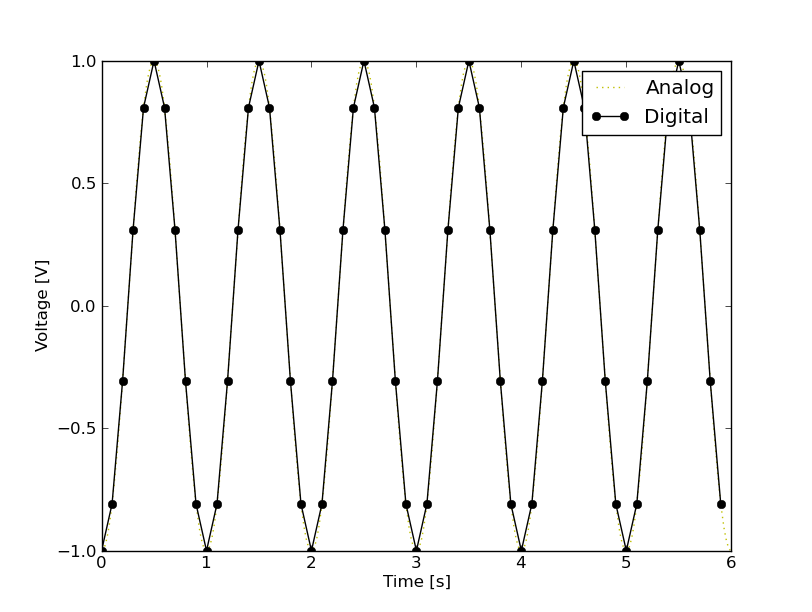
\includegraphics[width=\FigWidth\textwidth]{alias_x10.png}
\caption{A second illustration of the sampled signal from Figure~\ref{f:sample}. The ``Digital'' graph shows how the digital output of the A/D changes over time.  The reported value from the A/D only changes after each sampling event.}
\label{f:alias_x10}
\end{figure}

Now let's see how things change if we cut it close and use the minimum frequency ($f_s=\unit[2]{Hz}$), i.e., set the sampling frequency equal to twice the Nyquist frequency. Figure~\ref{f:alias_x1} illustrates that the sampled signal still roughly resembles the original sine wave, but things are starting to look a bit fishy.   
\begin{figure}[hbt!]
\centering
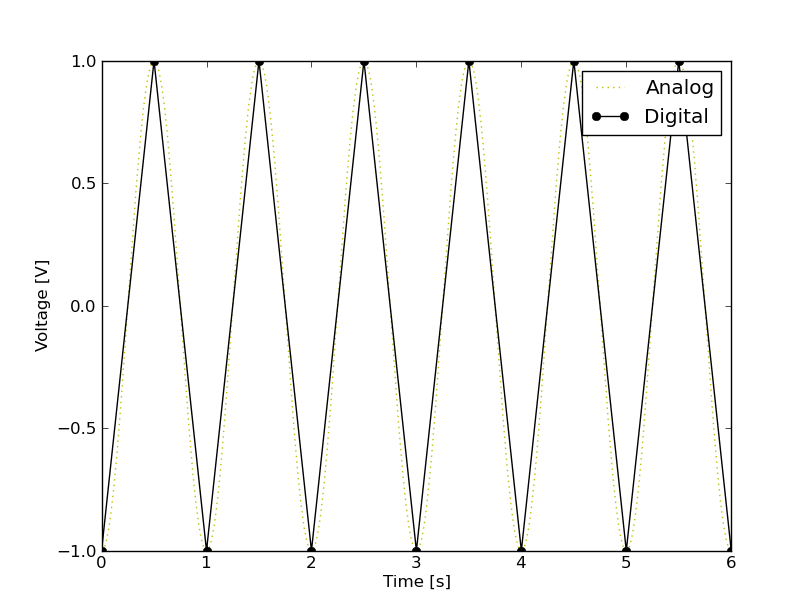
\includegraphics[width=\FigWidth\textwidth]{alias_x1.png}
\caption{Sampling at the minimum frequency, twice the Nyquist frequency: $f_s=\unit[2]{Hz}$, $dt=\unit[0.5]{s}$.}
\label{f:alias_x1}
\end{figure}

Finally, the sampling frequency becomes less than twice the Nyquist frequency the digital output is significantly different than the analog input.  Figure~\ref{f:alias_alias} illustrates that the digital output appears to be a sawtooth pattern with a much slower frequency of oscillation than the analog input, the term for this phenomenon is \gls{aliasing}.
\begin{figure}[hbt!]
\centering
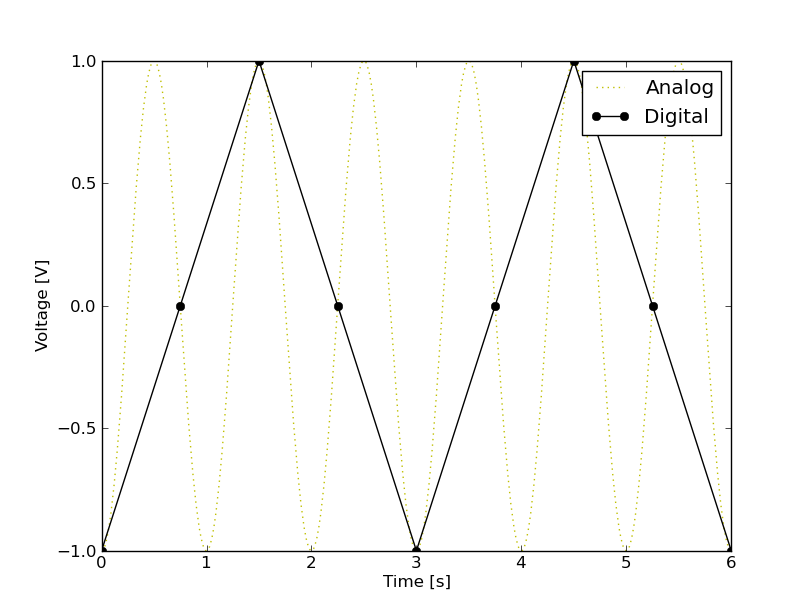
\includegraphics[width=\FigWidth\textwidth]{alias_alias.png}
\caption{Sampling below twice the Nyquist frequency: $f_s=\unit[1.33]{Hz}$, $dt=\unit[0.75]{s}$.}
\label{f:alias_alias}
\end{figure}

To generalize from our specific example, aliasing is when the analog input has significant frequency content above the half the sampling frequency.  These portions of the signal are folded back into the digital representation as lower frequency components that can corrupt the digital representation.  This can be a particular problem when there is high frequency noise.  In this case aliasing can cause high frequency noise to corrupt your lower frequency data.

To address this issue an anti-aliasing filter is often included in the signal conditioning portion of the data acquisition system.  This analog low-pass filter attenuates the higher frequency portions of the analog input, those portions of the input above the Nyquist frequency, to prevent these high frequency portions of the input from corrupting the measurement.

\begin{ex}
Anti-aliasing filters must be implemented on the analog signal.  However, digital filters can be used on the digital measurement (after the A/D conversion).  Why is it not possible to have a digital anti-aliasing filter?
\end{ex}




\printglossary[type=\thisgls]
\glsresetall

\renewcommand{\thisgls}{compare}
\newglossaryentry{qualitative comparison}
{
type=\thisgls,
name={qualitative comparison},
description={Comparing model predictions and experimental data based on subjective, non-numerical properties.}
}

\newglossaryentry{quantitative comparison}
{
type=\thisgls,
name={quantitative comparison},
description={Comparing model predictions and experimental data based on objective, numerical properties.}
}
\newglossaryentry{metric}
{
type=\thisgls,
name={metric},
description={Comparing model predictions and experimental data based on objective, numerical properties.}
}
\newglossaryentry{sample mean}
{
type=\thisgls,
name={sample mean},
description={Comparing model predictions and experimental data based on objective, numerical properties.}
}
\newglossaryentry{sample standard deviation}
{
type=\thisgls,
name={sample standard deviation},
description={Comparing model predictions and experimental data based on objective, numerical properties.}
}



\chapter{Model-Experiment Comparison}\label{c:compare}

In this chapter we'll discuss some general methods for comparing model predictions with experimental observations.  We are interested in being able to answer the questions, \emph{How good is the model?}, or more specifically, \emph{How good is the model at predicted the behavior of the physical system?}  We'll also present examples that show how these general concepts can be applied to particular models and experiments such as static and first-order models of physical systems like bending beams and temperature sensors.

We can make both \glspl{qualitative comparison} and \glspl{quantitative comparison} between model predictions and experimental data.  A qualitative comparison is based on subjective criteria such as does the time-response of our model ``look like'' the observed experimental data.  Qualitative evaluation is important, but it can only get us so far. As engineers we'll want to quantify our evaluation to put the comparison in subjective, numerical terms (hopefully with units!).  


\section{Quantitative Comparison}

\renewcommand{\ThisFigWidth}{0.3}
\begin{figure}[th!]
\centering
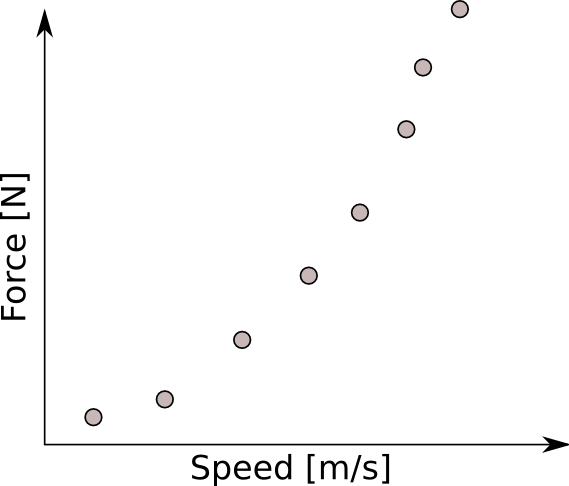
\includegraphics[width=\ThisFigWidth\textwidth]{model_fit_data.png}
\caption{Graph of our empirical measurements of pulling something through some fluid and measuring the drag force.  The individual data points are shown as circles.}
\label{f:modeldata}
\end{figure}

Let's consider an example.  Imagine we are measuring the drag force on something (a boat, surfboard, fish, diver, hang glider, etc.) as it moves through a fluid (air, water, mercury, etc.).  We pull our thing through our fluid at a few different speeds and measure the force.  If we plot our data it might look something like Figure~\ref{f:modeldata}.  Now that we have data, we might consider what type of (mathematical) model would be a good representation (or fit) to the model.  One thing we might try is to consider a \emph{linear model}, i.e., we are proposing that there is linear relationship between speed and drag force.  To be more specific, we are proposing that the function $F_{\mathrm{drag}}=m(V)$ could be a ``good'' representation of our observation.
\begin{figure}[hb!]
\centering
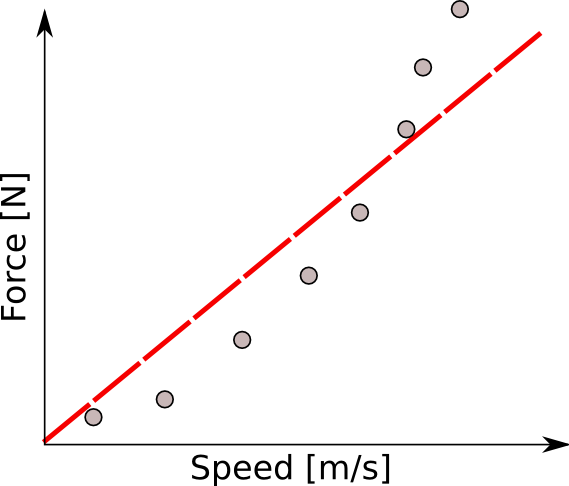
\includegraphics[width=\ThisFigWidth\textwidth]{model_fit_line.png}
\caption{Graph of our empirical measurements with a notional linear model.  The data (circles) and the linear model (red dashed line) are shown together.}
\label{f:modelline}
\end{figure}
Based on our data and our proposed model we could then come up with a value for the $m$ term in our model.  Figure~\ref{f:modelline} illustrates what this might look like.  Qualitatively this model ``looks pretty good'', but...

Alternatively, we might consider a different model.  Perhaps we could try a \emph{quadratic model} of the form $F_{\mathrm{drag}}=c(V^2)$.  Again, there is just one parameter in our model ($c$) that we'll need to choose so that the model and the data are similar. If we can find a reasonable quadratic coefficient we might get something that looks like Figure~\ref{f:modelquad}.  Based on this graph we could conclude, qualitatively, that the quadratic model is a ``better fit'' than the linear model.  We could also conclude that the error between the quadratic model and the data is ``small'', but we can't really get beyond these qualitative explanations.

\begin{figure}[bh!]
\centering
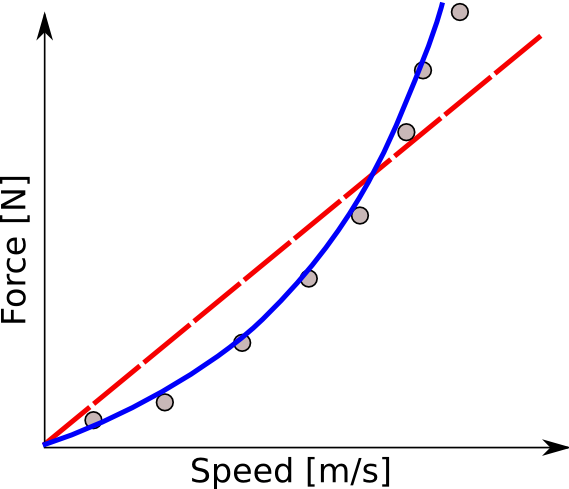
\includegraphics[width=\ThisFigWidth\textwidth]{model_fit_quad.png}
\caption{Graph of our empirical measurements with a notional linear and quadratic models.  The data (circles), linear model (red dashed line) and quadratic model (solid blue line) are shown together.}
\label{f:modelquad}
\end{figure}


\section{Quantitative Comparison}
Quantitative comparisons are based on \glspl{metric} (also known as a \emph{figure of merit}).  The metric is the numerical quantity (or quantities) that we are using to evaluate our comparison.  The type of model and experiment involved in the comparison of often dictates the types of metrics available.  In this section we'll present a few metrics that are useful for comparing the mathematical models and experiments typical in dynamic, mechanical systems.

\subsection{Simple Statistics}
We'll start with some simple (and hopefully familiar) statistical metrics.  Let's reconsider our example form Chapter~\ref{c:measure}, but this time we'll pretend we have a model.  Our ``model'' in this case is just a single prediction for the length of the fish we caught: $\hat{L}=\unit[1.0]{m}$.  (I'm not sure how we made this prediction, but we did.)  

Once we reel in our actual fish (our experiment) we use our digital ruler to make a series of measurements that we can summarize in Table~\ref{t:fishdata}. 
\begin{table}[bt!] 
\renewcommand{\arraystretch}{1.2}
\caption{Fishy Data}
\label{t:fishdata}
\centering
\begin{tabular}{|c|c|}\hline
Run & $L_i$ [m] \\ \hline \hline
1 & 0.76 \\ \hline
2 & 1.18 \\ \hline
3 & 1.17 \\ \hline
4 & 0.96 \\ \hline
5 & 1.48 \\ \hline
\end{tabular}
\end{table}
Remember, we are trying to compare our model ($\hat{L}$) with our data ($L_i$).  What could we say qualitatively?  We might say that is ``looks pretty good'', but that is very subjective.  One of our measurements is almost 50\% higher than our model prediction.  Is that ``pretty good'', ``fair'', ``poor'' or ``terrible''?

Luckily, we don't really have to make that decision.  Instead we can quantify the comparison.  One easy statistical quantity we can use is the \gls{sample mean} ($\bar{L}$) which can be expressed as
\begin{equation}\label{e:mean}
\bar{L} = \frac{1}{N}\sum_{i=1}^{N} L_i
\end{equation}
where $N$ is the number of samples (5 in this case) and $L_i$ is each of the $N$ samples (the data).  We might use the MATLAB \texttt{mean()} command to calculate $\bar{L}=\unit[1.11]{m}$.  Now we have a simple quantitative comparison, and we can say something like, ``The predicted value of $L$ was \unit[1.0]{m} and the sample mean of the measured length was \unit[1.11]{m} based on 5 samples, indicating an 11\% difference between the model and the experiment.''  As an engineer, this is a much more satisfying result that the comment that the ``data looks pretty close''---true?

Another simple statistic we can use to quantify our results is the \gls{sample standard deviation} of $L$ ($\sigma_L$) which can be expressed as
\begin{equation}\label{e:std}
\sigma_{L}=\sqrt{\frac{1}{N-1}\sum_{i=1}^{N}\left(L_i-\bar{L}\right)^2}.
\end{equation}
The standard deviation specifies how much variability in our data, indicating how much we can trust individual measurements.  We might use the MATLAB \texttt{std()} function to calculate the standard deviation of our measurements as $\sigma_L=\unit[0.24]{m}$, indicating that the expected variability in our measurements is roughly 24\% of the modeled value.  

\begin{table}[bt!] 
\renewcommand{\arraystretch}{1.2}
\caption{Summary of our fishy results}
\label{t:fishdata}
\centering
\begin{tabular}{|l|c|}\hline
Result & Value \\ \hline \hline
Predicted Length ($L$) & \unit[1.0]{m} \\ \hline
Mean Measured Length ($\bar{L}$) & \unit[1.11]{m} \\ \hline
Percent Difference: Model/Experiment & 11\% \\ \hline
Standard Deviation of Length Measurement ($\sigma_L$) & \unit[0.24]{m} \\ \hline
\end{tabular}
\end{table}

It is important to note a few things about our first example of quantitative comparisons:
\begin{itemize}
\item Our comparisons take the form of specific metrics
\item Our metrics have both numbers and engineering units
\item We can avoid having to make subjective judgments such as ``good'' or ``better''.
\end{itemize}

\subsection{Model Coefficients}
The previous simple statistics work well for scalar measurements where the underlying model is static (a single value).  However, in this book we are more interested in dynamic models and systems that change with time.  One way we can quantify these comparisons is by contrasting the predicted model coefficients with model coefficients based on our experiments.  

Let's consider an example based on our first-order model step response from Section~\ref{s:firststep}.  Let's assume we've come up with the mathematical model
\begin{equation}
\frac{dy(t)}{dt} + \frac{1}{\tau}y(t) = f(t),
\end{equation}
and we've predicted the time-constant is $\tau=\unit[10.0]{s}$ and the steady-state value is $Y_{ss}=\unit[100]{V}$.  Based on our model we can predict the step response as 
\begin{equation}\label{e:steppred}
y(t) = Y_{ss}\left(1-e^{-t/10.0}\right).
\end{equation}
Now we go into the lab and do a set of three experiments to magically measure the step response of our system.  If we graph our predicted response (\ref{e:steppred}) alongside our experimental observations we might get a plot similar to Figure~\ref{f:firstmodelex}.
\renewcommand{\ThisFigWidth}{0.4}
\begin{figure}[th!]
\centering
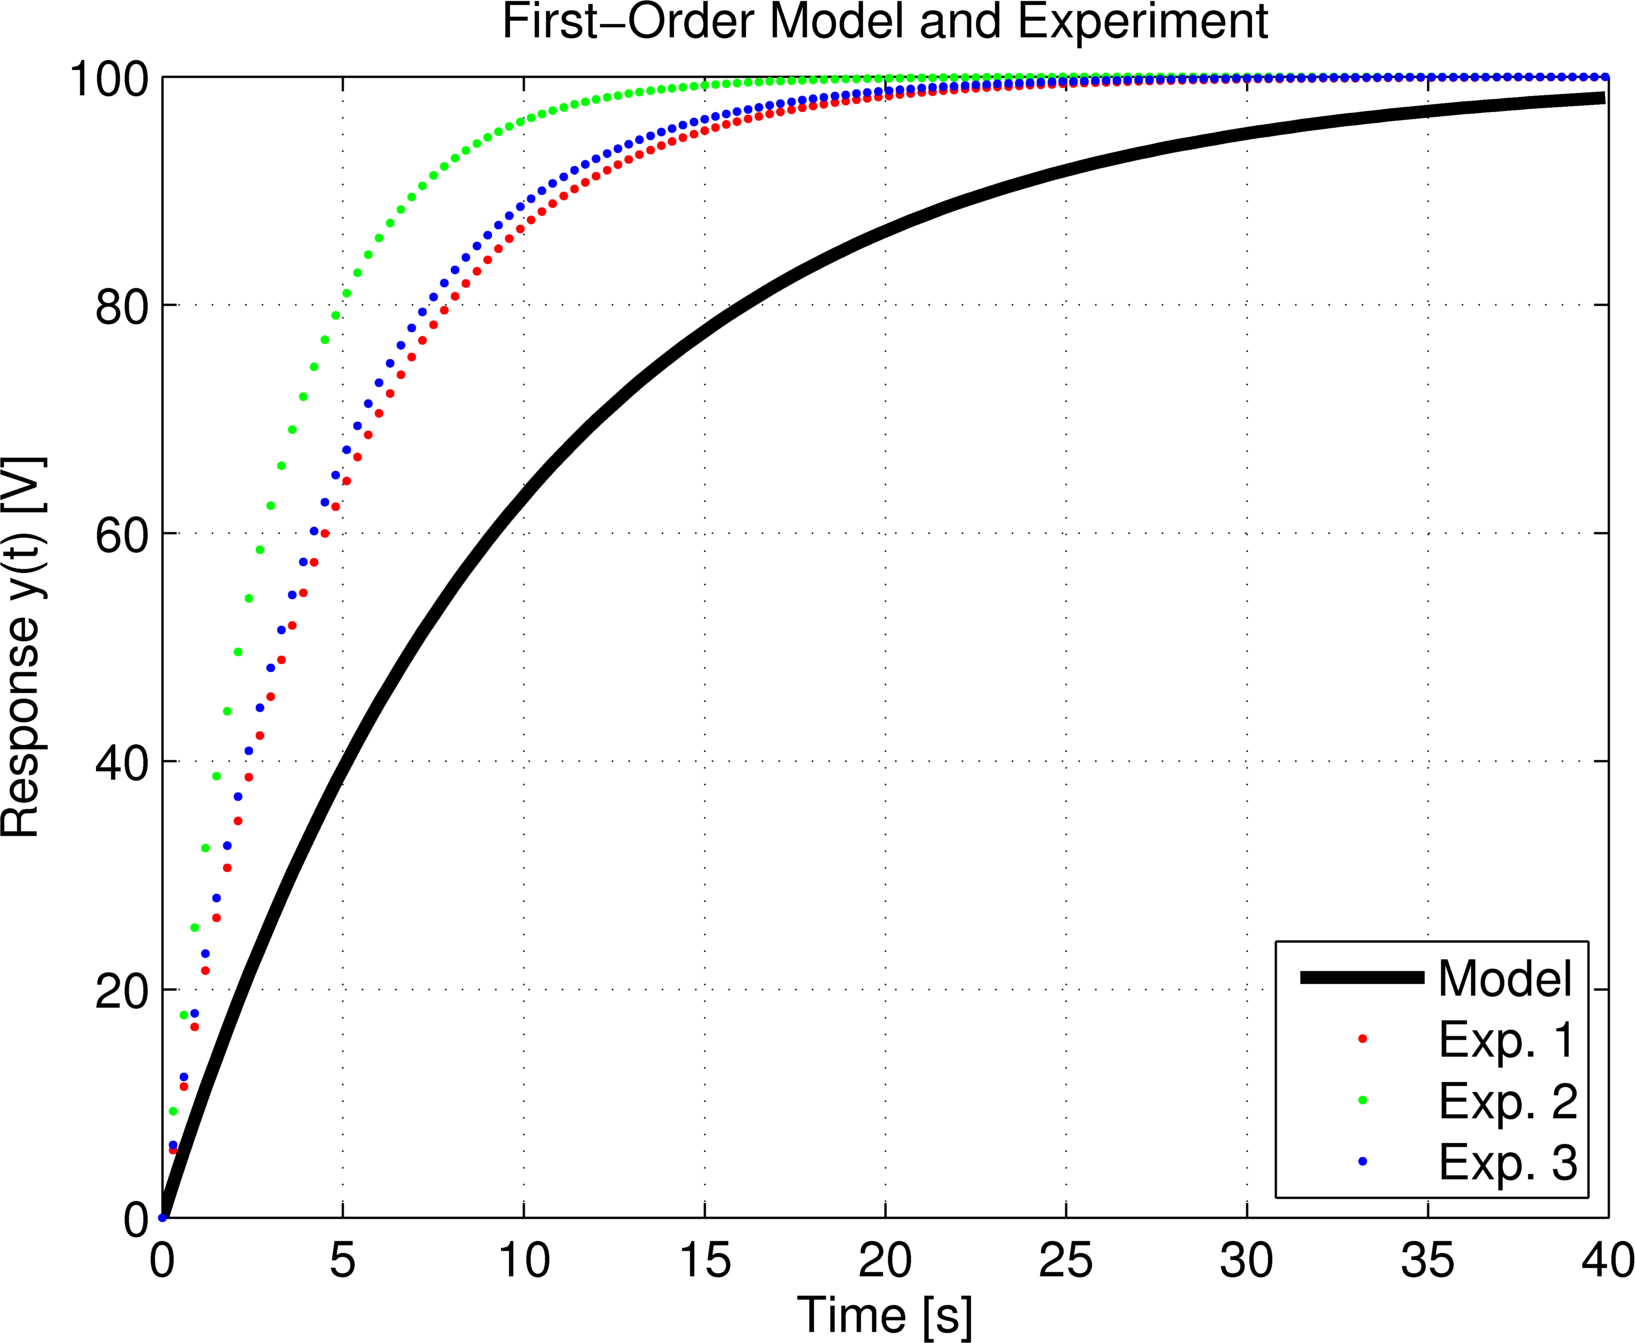
\includegraphics[width=\ThisFigWidth\textwidth]{first_modelex.png}
\caption{Illustration of our model prediction and experimental measurements.}
\label{f:firstmodelex}
\end{figure}
We can immediately make the following important qualitative comparisons:
\begin{itemize}
\item The model predicted steady-state response appears to agree with the empirical steady-state response.
\item The model predicted time constant appears to be larger than the experimentally measured time constant.
\end{itemize}
But, how do we quantify these comparisons?

One way to quantify the agreement between the model and the experimental results is to calculate a time constant based on the assumption that our physical experiment behaves like a first-order mathematical model. (Be careful here, a physical system does not have a time constant; only mathematical models have time constants!)  For each experimental trial we can estimate a time constant for the system.  Then we can compare the mean experimental time constant to the predicted time constant from the model and summarize the results in a table.
\begin{table}[bt!] 
\renewcommand{\arraystretch}{1.2}
\caption{Summary of our model predictions and experimental results}
\label{t:timec}
\centering
\begin{tabular}{|l|c|}\hline
Result & Value \\ \hline \hline
\textbf{Predicted Time Constant} & \textbf{\unit[10.0]{s}} \\ \hline
Experimental Time Constant: Run 1 & \unit[4.2]{s} \\ \hline
Experimental Time Constant: Run 2 & \unit[4.5]{s} \\ \hline
Experimental Time Constant: Run 3 & \unit[2.8]{s} \\ \hline
\textbf{Experimental Time Constant: Mean} & \textbf{\unit[3.8]{s}} \\ \hline
Difference, Model vs. Exp. Time Constant & \unit[6.2]{s} \\ \hline
\textbf{Percent Error} & \textbf{62\%} \\ \hline
\end{tabular}
\end{table}

One thing to be specific about is how we calculate the \emph{percent error} in Table~\ref{t:timec};
\[
\%\,\mathrm{Error}=\frac{|\mathrm{Experimental}-\mathrm{Theoretical}|}{\mathrm{Theoretical}}.
\]

\printglossary[type=\thisgls]
\glsresetall

\renewcommand{\thisgls}{strain}
\newglossaryentry{strain gage}
{
type=\thisgls,
name={strain gage},
description={In general, a strain gage is a sensor (a transducer) that transforms strain into a measureable quantity.  For our purposes a strain gage refers to a metallic foil strain gage bonded to the surface of a structure.  This type of strain gage changes resistance in response to an applied deformation in a known way}
}

\newglossaryentry{bridge excitation voltage}
{
type=\thisgls,
name={excitation voltage},
description={Also known as the supply voltage.  This is the constant, known voltage applied to a Wheatstone bridge.}
}



\chapter{Case Study: Beam Response and Stain Gage}\label{c:strain}

In this chapter we will work through and example data acquisition design problem.  Our goal is present a complete system, with as much detail as possible, capable of measuring the response (static and dynamic) of a cantilevered beam subject to a load.

\section{Static Model: Cantilevered Beam}

Figure~\ref{f:cant} shows the solution to the classical beam equation for a cantilevered beam with a load placed at the tip.  This simple case illustrates how we can predict the moment ($M(x)$) and deflection ($y(x)$) in the structure as a function of the applied load.

\begin{figure}[hb!]
\centerline{
{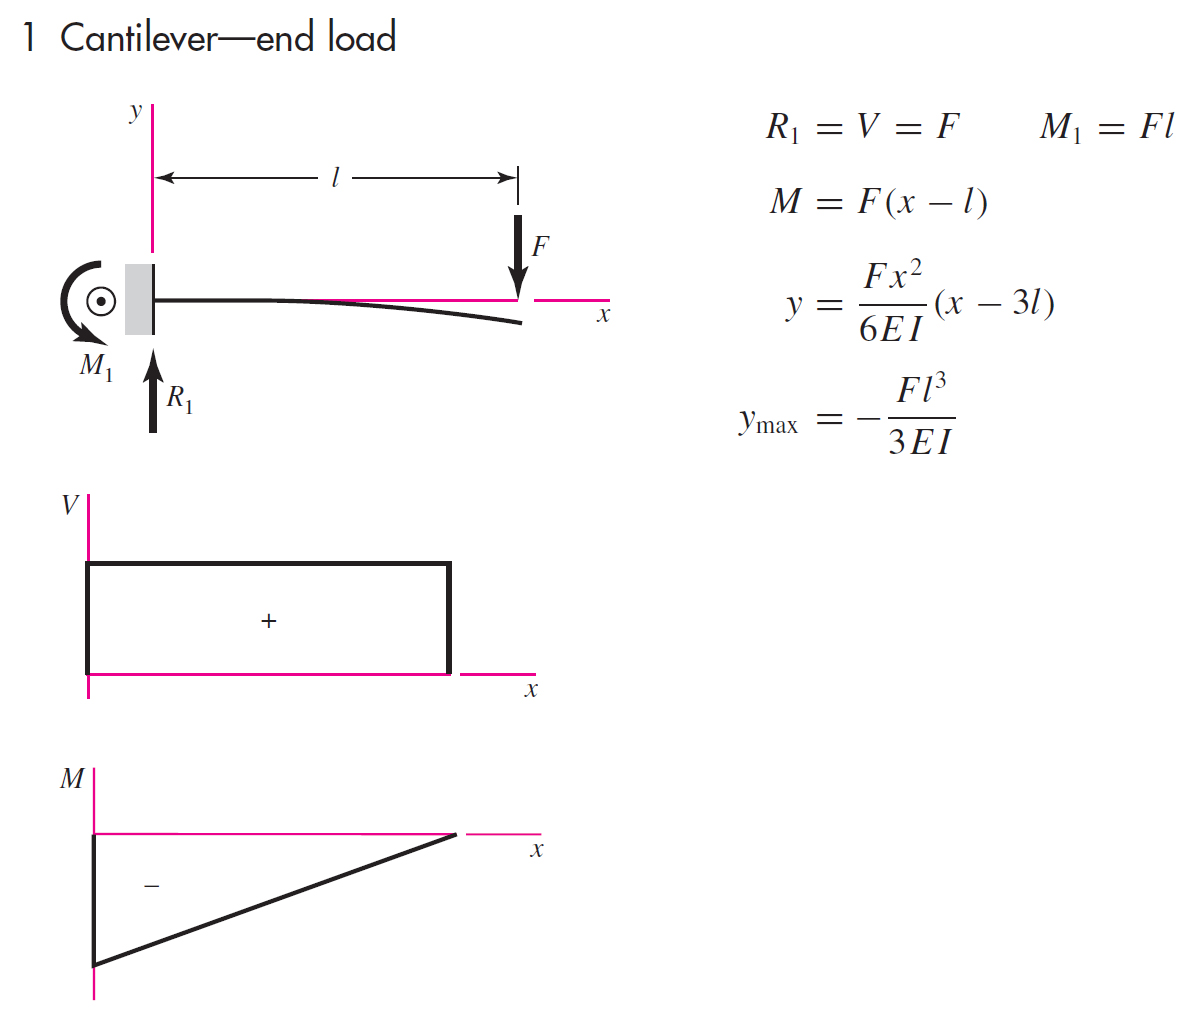
\includegraphics[width=0.5\textwidth]{cant_beam.jpg}}}
\caption{Shear, moment and deflection of a cantilevered beam.  Courtesy of \emph{Shigley's Mechanical Engineering Design}, 8th Edition, Budynas and Nisbett.}
\label{f:cant}
\end{figure}


\subsection{Determining Strain and Displacement}
Two quantities of the response of the beam that we'd like to be able to predict is the strain ($\epsilon$), due to bending, at a particular location along the length ($x$) as a function of the applied load ($F$) and the displacement at the free end of the beam ($y_{max}$) as a function of the applied load.  We can start with the (hopefully) familiar expression for bending stress in a beam due to an applied moment,
\[
\sigma_x=\frac{M(h/2)}{I}
\]
where $h$ is the height of the beam cross-section and $I$ is the second moment of area of the beam cross-section.  We can use the linear relationship for elastic stress and strain ($\sigma_x = E \epsilon$) to find an expression for the strain at any location $x$ along the beam.
\[
\epsilon = \frac{F(x-l)(h/2)}{EI}
\]
We can then solve for the tip force and the tip displacement as a function of the measured strain:
\begin{equation}\label{e:strainf}
F = \left( \frac{EI}{(x-l)(h/2)} \right) \epsilon 
\end{equation}
\begin{equation}\label{e:straine}
y_{max}=\left( \frac{l^3}{3(x-l)(h/2)} \right) \epsilon.
\end{equation}
These two equations are models of the response of a cantilevered beam. The first model (\ref{e:strainf}) predicts the force at the free end of the beam ($F$) as a function of the strain.  The second model (\ref{e:straine}) predicts the displacement at the free end of the beam as a function of the strain.

\section{Sensor: Strain Gage}
In our example we are going to use a stain gage to measure the deformation (strain) at one location in our bending beam.  Based on this estimate of deformation we can infer the strain and stress in the structure as well as the motion of the beam.  The sensor we will use is a \gls{strain gage} or more specifically, a bonded resistance strain gage.  This sensor, illustrated in Figure~\ref{f:strain} is a very common measurement tool for mechanical systems.  The type of strain gage we are considering is bonded to a surface so that when that element is deformed, the strain gage is deformed by the same amount.  This deformation causes the resistance of the foil grid (see Figure~\ref{f:strain}) to change according to the relationship
\begin{equation}\label{e:gage}
\mathrm{GF} = \frac{\delta R / R}{\delta L / L}=\frac{\delta R /R}{\epsilon}
\end{equation}
where $R$ is the nominal resistance of the strain gage (e.g., \unit[120]{Ohms}), $\delta R$ is the change in resistance, $L$ is the length of the gage, $\delta L$ is the change in length and $\epsilon$ is the strain at the location of the gage.  For metallic foil strain gages, GF is typically close to 2.  Since the stain in engineering devices is usually less than 1\%, which suggests that the change in resistance in a strain gage is very small, typically less than 1\%.  

\begin{figure}[hb!]
\centerline{
{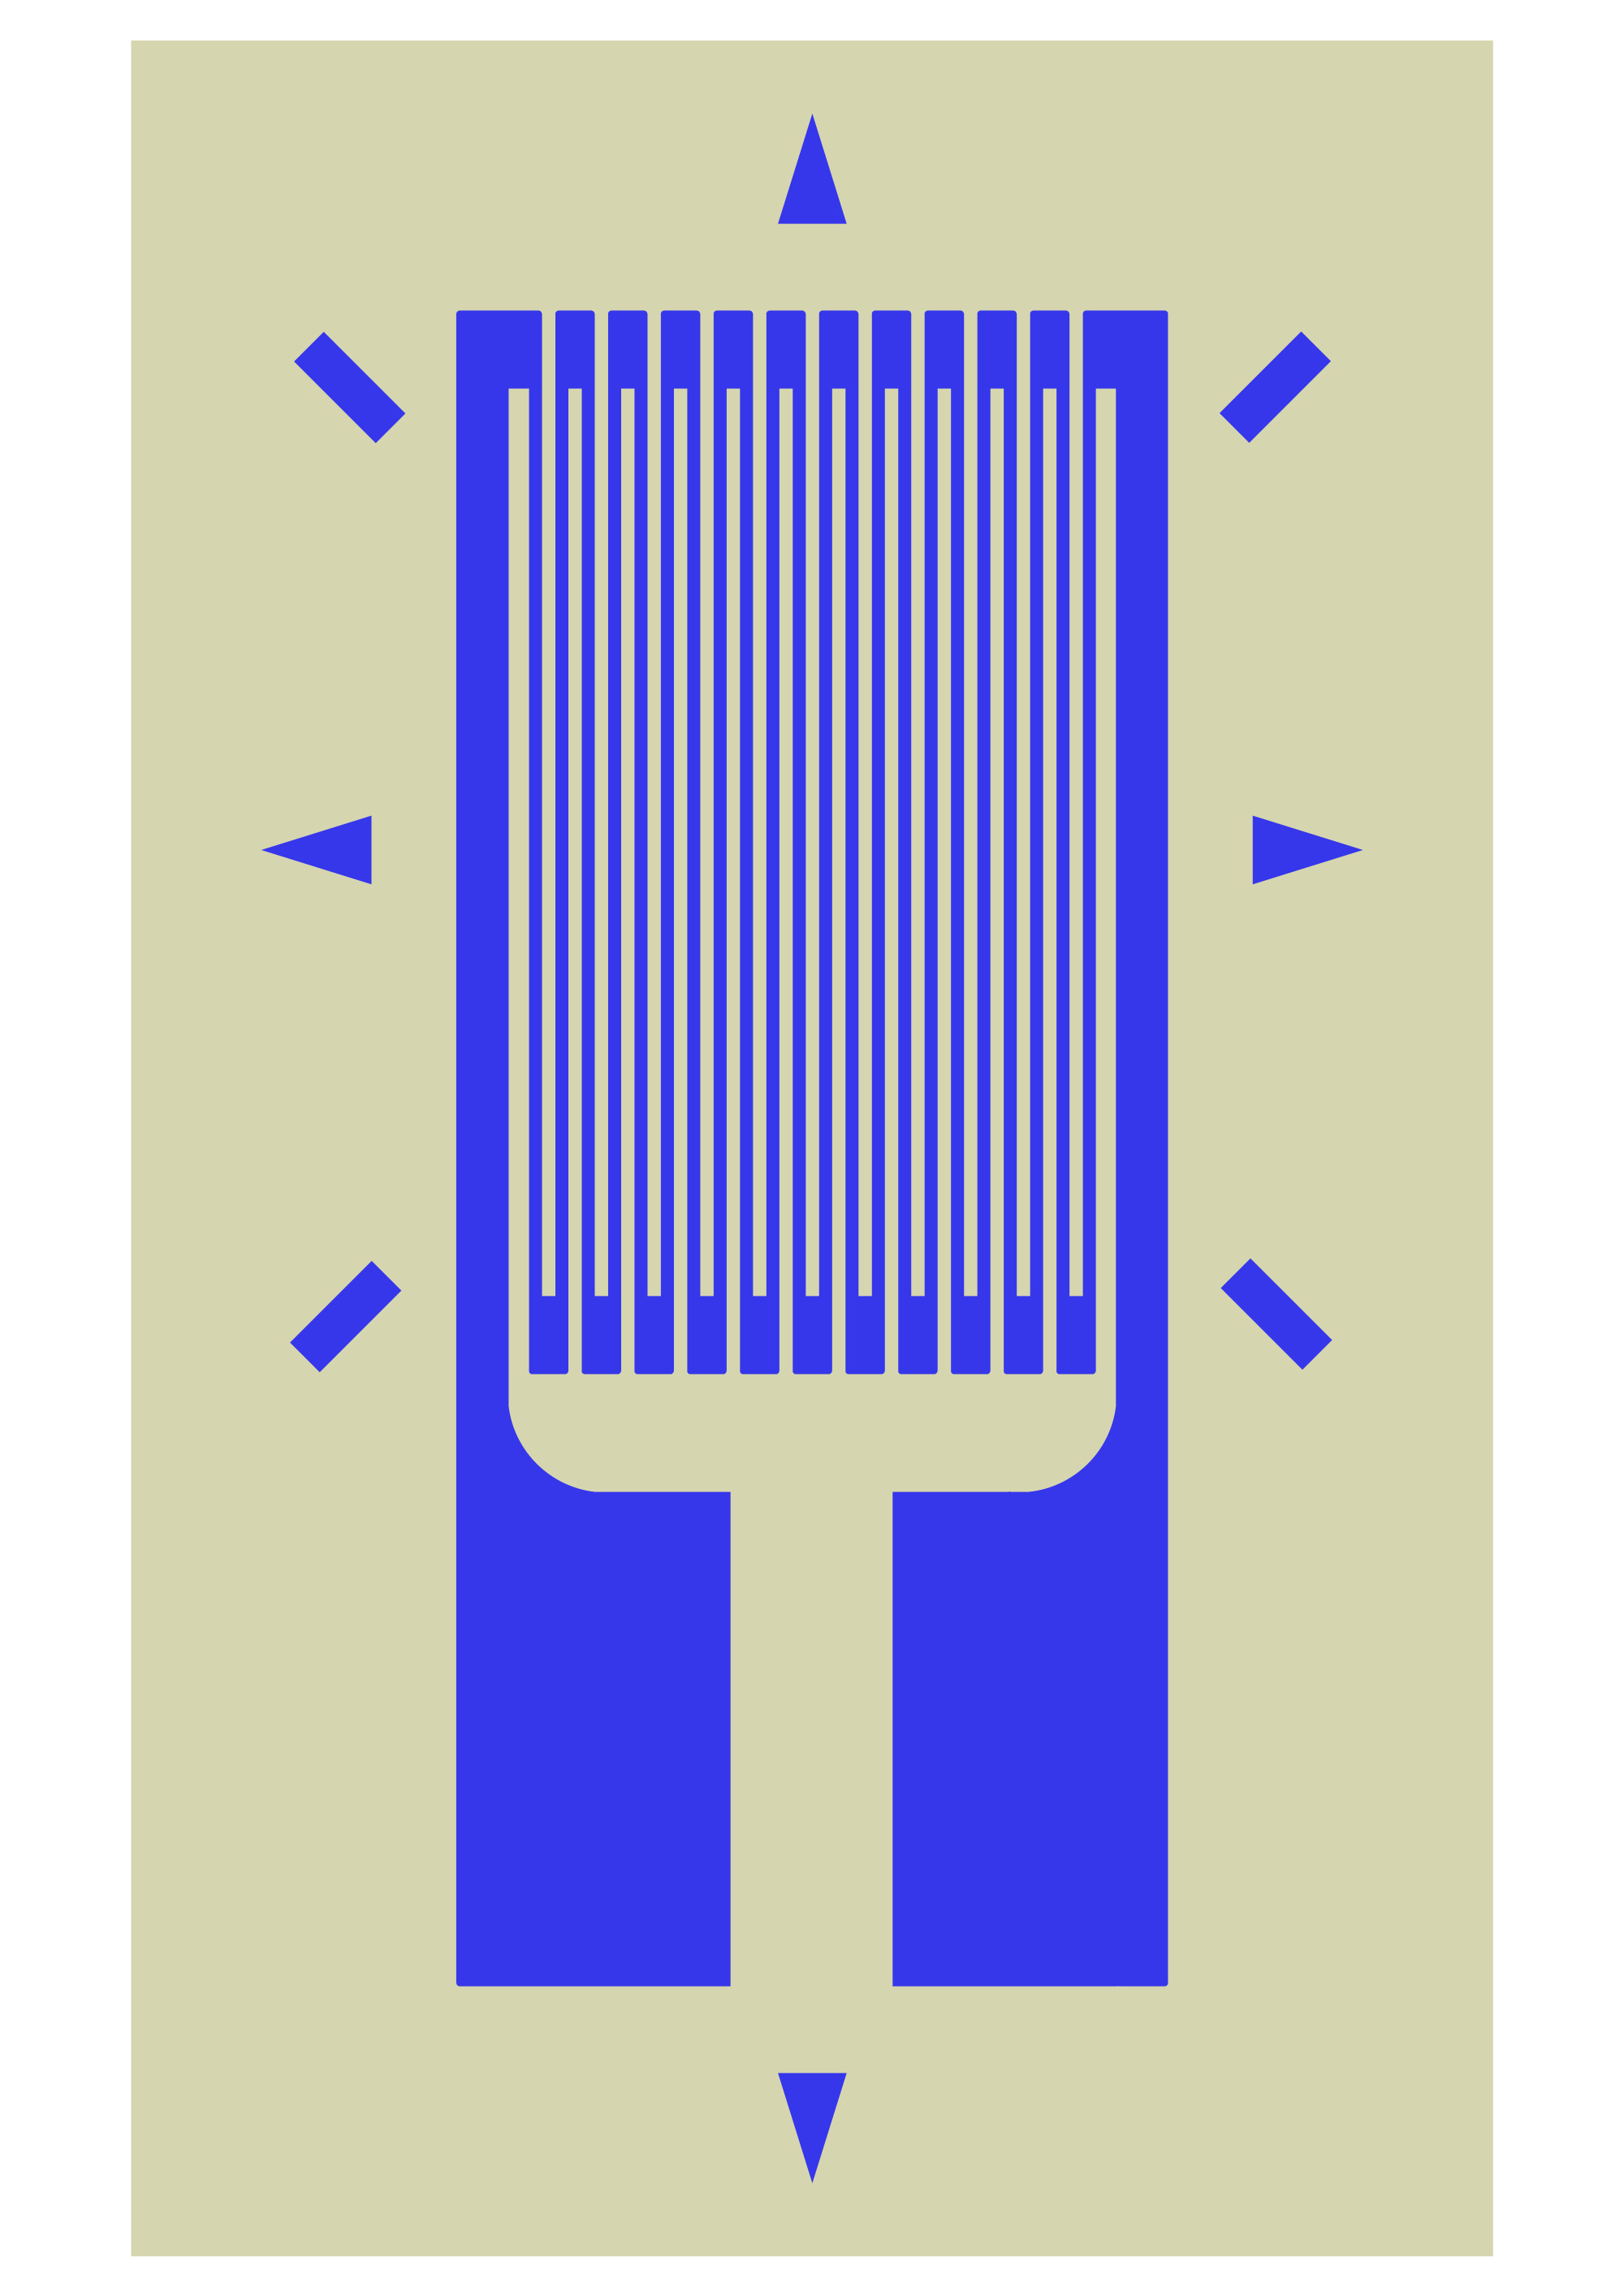
\includegraphics[width=0.4\textwidth]{strain.png}}}
\caption{Schematic of a typical metallic foil strain gage.  (This image is by ``MADe'', is licensed under the CC BY-SA license and is available from \url{http://en.wikipedia.org/wiki/File:Strain_gauge.svg}) }
\label{f:strain}
\end{figure}


\section{Signal Conditioning: Wheatstone Bridge}
The strain gage is one of many sensors where the transduction is a conversion to a small change in resistance.  Directly measuring such a small resistance within a data acquisition system is challenging.  It would be preferable if the input to our analog to digital converter was a voltage indicating the value of the physical quantity we are attempting to measure.  Enter the Wheatstone bridge.  This simple circuit is sketched in Figure~\ref{f:bridge}.  This particular implementation illustrates a ``quarter-bridge'' circuit, where the sensor is represented by the resistor value $R_x$.

\begin{figure}[hbt!]
\centerline{
{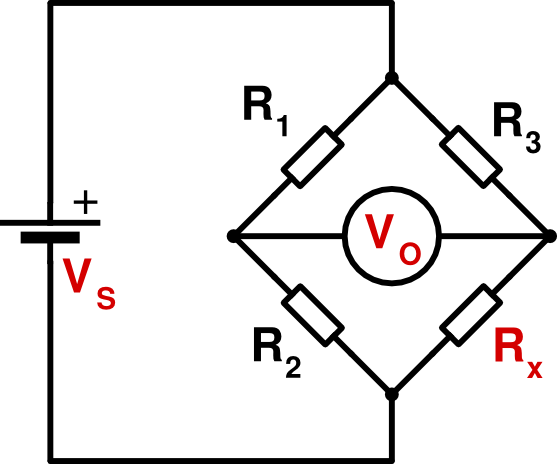
\includegraphics[width=0.5\textwidth]{Wheatstonebridge2.png}}}
\caption{  (This image an adaptation of the image by ``Zedh'', is licensed under the CC BY-SA license and is available from \url{http://en.wikipedia.org/wiki/File:Wheatstonebridge.svg}) }
\label{f:bridge}
\end{figure}

To get started, consider if the bridge is perfectly ``balanced'' which requires all the resistance values ($R_1$, $R_2$, $R_3$ and $R_x$) to be equivalent.  The \gls{bridge excitation voltage} ($V_S$) is applied as shown (e.g., $V_s=\unit[10]{V}$).  (The excitation voltage could also be called the supply voltage.) The output of the bridge circuit is $V_o$.  Given this scenario, with the bridge in a balanced state, what is the output voltage?  Hopefully it makes conceptual sense that this voltage would be zero.  Since the all the resistors are of the same value the voltage drop across each resistor would be equivalent.

When the value of one leg of the bridge changes, say when a strain induces a change in resistance of $R_x$, then the bridge us unbalanced and the output voltage is non-zero.  We won't do the circuit analysis here (there are plenty of examples online if you are interested), and instead we'll just present the result:
\begin{equation}\label{e:bridge}
V_o = V_s \left( \frac{\delta R_x/R_x}{4+2(\delta R_x/R_x)} \right) \approx \frac{\delta R_x/R_x}{4}.
\end{equation}
This expression quantifies how a change in resistance of one leg of a quarter-bridge circuit is converted into a corresponding output voltage.  One thing to not is that the sensitivity of the bridge circuit is a function of of the excitation voltage ($V_s$).  So, the larger the excitation the larger the output voltage, for an equivalent change in resistance.  (Of course the larger the supply voltage the larger the current flowing through the bridge which results in unnecessary heating which then causes other problems.)

There are other implementations of the Wheatstone bridge such as half-bridge and full-bridge configurations; we'll stick with the quarter-bridge for now.

\section{Strain Gage Data Acquisition}
\begin{figure}[hbt!]
\centering
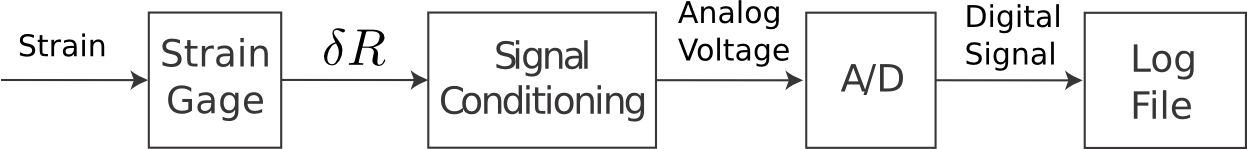
\includegraphics[width=\FigWidth\textwidth]{strain_daq.png}
\caption{A data acquisition including a strain gage and Wheatstone bridge.  See Figure~\ref{f:daq} for the general DAQ layout.}
\label{f:straindaq}
\end{figure}

By putting these components together we can build a complete data acquisition system for measuring strain as illustrated in Figure~\ref{f:straindaq}. To describe the mathematical relationship between physical strain and the analog voltage measured by the A/D we combine (\ref{e:gage}) and (\ref{e:bridge}) to generate the expression
\begin{equation} \label{e:gagebridge}
V_o \approx V_s\left( \frac{(\mathrm{GF})\epsilon}{4} \right).
\end{equation}

\section{Exercises}
\begin{ex}
Using (\ref{e:strainf}) and (\ref{e:gagebridge}) derive a mathematical model (an equation) that predicts the voltage output of the Wheatstone bridge ($V_o$) as a function of the applied load at the free end of the beam.
\end{ex}


























\printglossary[type=\thisgls]
\glsresetall

\renewcommand{\thisgls}{linear}
\newglossaryentry{tmp}
{
type=\thisgls,
name={tmp},
description={In general, a strain gage is a sensor (a transducer) that transforms strain into a measureable quantity.  For our purposes a strain gage refers to a metallic foil strain gage bonded to the surface of a structure.  This type of strain gage changes resistance in response to an applied deformation in a known way}
}




\chapter{Static Linear Model}\label{c:linear}

One very common model for the static response of a system is the familiar equation of a line
\begin{equation}\label{e:line}
y = m*x+b
\end{equation}
where $x$ is the input, $y$ is the output, $m$ is the slope and $b$ is the y-intercept.  To put this in context of the dynamic linear models (e.g., first and second order) this model is referred to as a zero-order differential equation
\begin{equation}\label{e:zero}
y(t) = m*x(t)+b.
\end{equation}

One example of a physical system that can be approximated using this type of model is a mass-spring-damper idealization as shown in Figure~\ref{f:msd}.  We can consider either the dynamic response (which we'll model later as a second-order model) or the static response.  The static response ($x(t)$) to an input force ($F(t)$ of such a system can be approximated by Hooke's law
\begin{equation}\label{e:hooke}
x(t) = 1/K*F(t)
\end{equation}
where $K$ is the spring constant for the spring, $x(t)$ is the static displacement and $F(t)$ is the constant applied force.  Keep in mind that this is only reasonable for the \emph{static} scenario; if $F(t)$ is not constant this will be a very poor model to predict the response $x(t)$.

\begin{figure}[htb!]
\centerline{
{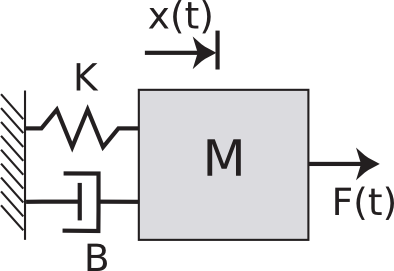
\includegraphics[width=0.4\textwidth]{msd_icon.png}}}
\caption{Sketch of a mass-spring-damper system.}
\label{f:msd}
\end{figure}


\section{Static Calibration}
In order to use a model such as (\ref{e:hooke}) we need to know the unknown parameters in the model, for example the spring constant $K$.  Static calibration is the process of experimentally determining this value.  If we know that the system is perfectly linear (which systems never are) and that our measurements are perfect (which they never are) this process is very simple.  All we have to do is...
\begin{itemize}
\item Apply a known static load $F$
\item Measure the resulting static displacement $x$
\item Substitute these values into (\ref{e:hooke}) and solve for $K$
\end{itemize}
This works surprisingly well if we are confident of our model (linearity) and our measurements.  However, to be a little more cautious we might want to repeat this process a few times at various known static loads and then combine all that data to determine a best-fit value for $K$ based on more than one measurement.  This process is known as \emph{fitting a model to the data}.

\section{Least-Squares Regression}
Regression analysis can be used to \emph{fit} model to experimental data.  For regression analysis the static model is a polynomial of order $m$ such as
\begin{equation}\label{e:rmodel}
\hat{y} = a_0+a_1*x+a_2*x^2+\ldots+a_m*x^m
\end{equation}
where $\hat{y}$ is the response predicted by the model.  Consider the linear case ($m=1$) illustrated in Figure~\ref{f:linear} where the model takes the form
\begin{equation}
\hat{x} = a_0 + 1/K*F
\end{equation}
and the experimental measurements are $x_i$ for each input $F_i$.  

\begin{figure}[hb!]
\centerline{
{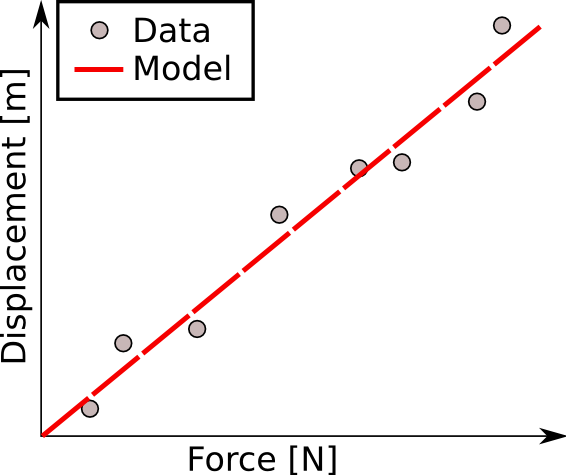
\includegraphics[width=0.4\textwidth]{linear_model_fit.png}}}
\caption{Illustration of a set of experimental measurements (data) and the best-fit linear model.}
\label{f:linear}
\end{figure}


In this case there are eight data points so $i=1,2,\ldots,8$.  The most common method to determine a the parameters of the model that best-fit the data is to minimize square-error between the prediction and the measurement at each test input.  In other words, the \emph{method of least-squares} finds values for $a_0$ and $K$ to minimize the quantity
\begin{equation}
L = \sum_{i=1}^N \left(x_i - \hat{x}_i \right)^2.
\end{equation}


Exactly how to accomplish this is beyond the scope of this book, but there are many tools (MATLAB, MS-Excel, etc.) that will solve this problem and provide you with a quantification of the \emph{goodness-of-fit}.  The first of these parameters is the \emph{coefficient of determination}, $R^2$, which defines, ``how much of the variance in the data is described by the linear fit''.  The $R^2$ parameter is between 0--1, with values greater than 0.9 indicated a good degree of fit (or agreement) between the data and the model.  Another way to quantify the comparison between the model and the data is to compute the \emph{standard error of the fit} as
\begin{equation}\label{e:standerror}
s = \sqrt{\frac{\sum_{i=1}^N \left(x_i - \hat{x}_i \right)^2}{\nu}}
\end{equation}
where $\nu$ is the degrees of freedom of the fit and $\nu=N-(m+1)$.  For our linear example ($m=1$) with eight data points ($N=8$), $\nu=8-(2)=6$. 

\printglossary[type=\thisgls]
\glsresetall

\renewcommand{\thisgls}{model2}
\newglossaryentry{second-order model}
{
type=\thisgls,
name=second-order model,
description={A linear, ordinary, time-invariant, second-order differential equation.}
}

\newglossaryentry{damping ratio}
{
type=\thisgls,
name=damping ratio,
description={},
symbol={$\zeta$}
}

\newglossaryentry{undamped natural frequency}
{
type=\thisgls,
name=undamped natural frequency,
description={},
symbol={$\omega_n$}
}

\newglossaryentry{damped natural frequency}
{
type=\thisgls,
name=damped natural frequency,
description={},
symbol={$\omega_d$}
}

\chapter{Dynamic Models: Part 2}\label{c:model2}
So far we have examined two mathematical models to predict and quantify the response of mechanical systems: a static (zero-order) model and a first-order dynamic model.  It may not be terribly surprising that our next topic is a second-order model.  A second-order model is a generic mathematical description of a system that is capable of oscillations. (You might recall that neither a static response nor a first-order response oscillates.)   This simple model can be used to help understand the behavior of a variety of engineering systems such as
\begin{itemize}
\item pendulums, where the position oscillates
\item passive circuits, where the voltage/current oscillates 
\item acoustic systems, where the sound pressure level (volume) oscillates.
\end{itemize}

The key elements of a second-order model are \emph{inertia}, \emph{stiffness} and \emph{damping} where the interpretation of these elements depends on the domain (mechanical, electrical, acoustic, etc.) under examination.  We will focus on mechanical systems where the inertia is in the form of mass, the stiffness is a restoring force (such as a spring or gravity) and damping is losses due to frictional forces.


\section{Second-Order Model}
We will use \gls{second-order model} as shorthand for a linear, ordinary, time-invariant second-order differential equation of the form
\begin{equation} \label{e:second}
\ddot{y}(t) + 2 \zeta \omega_n \dot{y}(t) + \omega_n^2 y(t) = f(t)
\end{equation} 
where 
\begin{itemize}
\item $\ddot{y}(t)$ is the second derivative of $y(t)$ with respect to time,
\item $\dot{y}(t)$ is the first derivative of $y(t)$ with respect to time,
\item $y(t)$ is the solution to (\ref{e:second}),
\item $\zeta$ is the \gls{damping ratio},
\item $\omega_n$ is the \gls{undamped natural frequency} and
\item $f(t)$ is the input, or forcing function.
\end{itemize}
Just as with our first-order and static (zero-order) models, this model is an abstraction; it never has exactly the same behavior of a physical system, but it has been proven to be a useful approximation for the behavior of a variety of phenomena.  To understand the model we'll first present the solution to (\ref{e:second}) for a few types of input (forcing functions) and then work through some examples of cases where the model is a helpful abstraction of physical systems.

The intent of the following discussion is meant to be a summary and/or review of what you have seen in other courses (Differential Equations, System Dynamics, Feedback Controls, etc.).  The discussion should be sufficient for our purposes of modeling and measurement, but it is by no means an exhaustive treatment of analysis of second-order models or harmonic oscillator models.

Also, for now we are only interested in {\bf underdamped} and {\bf undamped} versions of the model (\ref{e:second}) where $0 \leq \zeta < 1.0$.  Another way to say this is that we are only interested in second-order models that have oscillations in their response.

\subsection{Example: Mass-Spring-Damper}
One type of physical system that has similar behavior to our second-order model is the mass-spring-damper system illustrated in Figure~\ref{f:msd2}.  (Actually, this system is still a bit of an abstraction; we rarely encounter applications that require a point mass attached to a mass-less spring.  The abstraction is meant to represent any physical system where there is inertia (mass, kinetic energy), a restoring force (spring, potential energy) and motion resistance (damper, energy dissipation).)
\begin{figure}[htb!]
\centerline{
{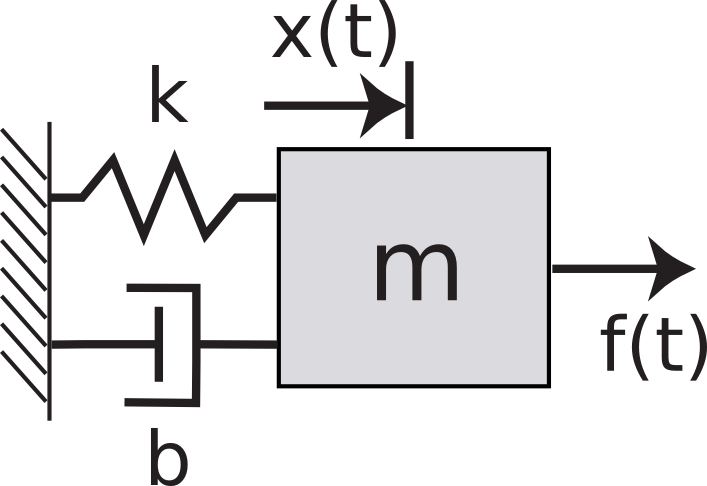
\includegraphics[width=0.4\textwidth]{msd_lower.png}}}
\caption{Sketch of a mass-spring-damper system.}
\label{f:msd2}
\end{figure}

If you draw a free-body-diagram of this system, you should be able to derive the second-order equation of motion
\begin{equation}\label{e:msd}
m \ddot{x}(t) + b \dot{x}(t) + k x(t) = f(t)
\end{equation}
where $m$ is the mass, $b$ is the linear damping coefficient, $k$ is the linear spring constant, $x(t)$ is the displacement of the mass and $f(t)$ is the input force.

\begin{ex}
Using (\ref{e:second}) and (\ref{e:msd}), derive expressions for the system parameters ($\omega_n$ and $\zeta$) in terms of the physical parameters ($m$, $b$, and $k$).  (Hint: Use physical units to check your answers.)
\end{ex}

\ifsolutions
\begin{soln}
You should verify that the following expressions are correct:
\[ \omega_n = \sqrt{k/m} \; \; \; \unitfrac[]{rad}{s}\]
\[ \zeta = \frac{b}{2 \sqrt{mk}} \; \; \; \unitfrac[]{n}{a} \]
\end{soln}
\fi


\section{Free Response}\label{s:secondfree}
The free response for our model is the solution to the second-order model (\ref{e:second}) with initial conditions, but no forcing function (also known as the homogeneous equation)
\begin{equation} \label{e:secondhomo}
\ddot{y}(t) + 2 \zeta \omega_n \dot{y}(t) + \omega_n^2 y(t) = 0
\end{equation} 
where the initial conditions at $t=0$ are
\begin{itemize}
\item $y(0) = y_o$ and 
\item $\dot{y}(0)=\dot{y}_o$.
\end{itemize}
Hopefully you've been convinced that this type of differential equation is straightforward to solve (in theory), and we can present (without derivation) that the solution to this equation is the function
\begin{equation} \label{e:secondfree}
y(t) = C \left(e^{-\zeta \omega_n t}\right) \left( \cos(\omega_d t - \phi) \right).
\end{equation}
where
\begin{eqnarray}\
\omega_d & = & \omega_n \sqrt{1-\zeta^2}, \label{e:damped} \\
C & = & \sqrt{ y_o^2 + \left( \frac{\dot{y}_o+\zeta\omega_n y_o}{\omega_d} \right)^2 } \;\;\;\;\;\;\;\;\; \mathrm{and}\label{e:C} \\
\tan(\phi) & = & \frac{\dot{y}_o+\zeta \omega_n y_o}{\omega_d y_o}. \label{e:phi}
\end{eqnarray}

The free response (\ref{e:secondfree}) is the key part of all this.  There are many systems that behave in this general way with a decaying oscillatory response.  To illustrate this we can annotate the equation to highlight the three parts of the solution:
\begin{equation} \label{e:secondfree_annote}
y(t) = \underbrace{C}_\text{constant} 
\underbrace{\left(e^{-\zeta \omega_n t}\right)}_\text{exponential decay}
\underbrace{\left( \cos(\omega_d t - \phi) \right)}_\text{oscillation}.
\end{equation}
One important detail is that there are two slightly different ``natural frequencies'' to keep track of.  The \gls{undamped natural frequency} ($\omega_n$) is the parameter we saw in the system model and which is included in the exponential decay component of (\ref{e:secondfree_annote}).  The \gls{damped natural frequency} ($\omega_d$) is the frequency of oscillation, the angular frequency inside the $\cos$ term of (\ref{e:secondfree_annote}).  The relation between the two values is given in (\ref{e:damped}).  For small values of $\zeta$, so called ``lightly damped systems'', there is little difference between the two values.

Another way to ``see'' this solution is to graph the time response.  The short MATLAB script in Listing~\ref{l:secondfree} generates Figure~\ref{f:secondfree}.  This figure illustrates the key characteristics of a second order free response:
\begin{enumerate}
\item the system oscillates at a constant frequency (the $\cos(\omega_d t)$ term) and
\item the amplitude of the oscillations decays exponentially over time (the $e^{=\zeta \omega_n t}$ term).
\end{enumerate}
%\lstinputlisting[style=myMatStyle,
%caption={Script for plotting the free response of a second-order model (\verb+second_order_free.m+).},
%label={l:second_free}]
%{./code/second_order_free.m}

\lstinputlisting[style=myMatStyle,
caption={Script for plotting the free response of a second-order model. (Filename=second\_order\_free.m, \url{http://web.eng.hawaii.edu/~bsb/me402/book/code/second_order_free.m})},
label={l:secondfree}]
{../code/second_order_free.m}


\begin{figure}[hbt]
\centering
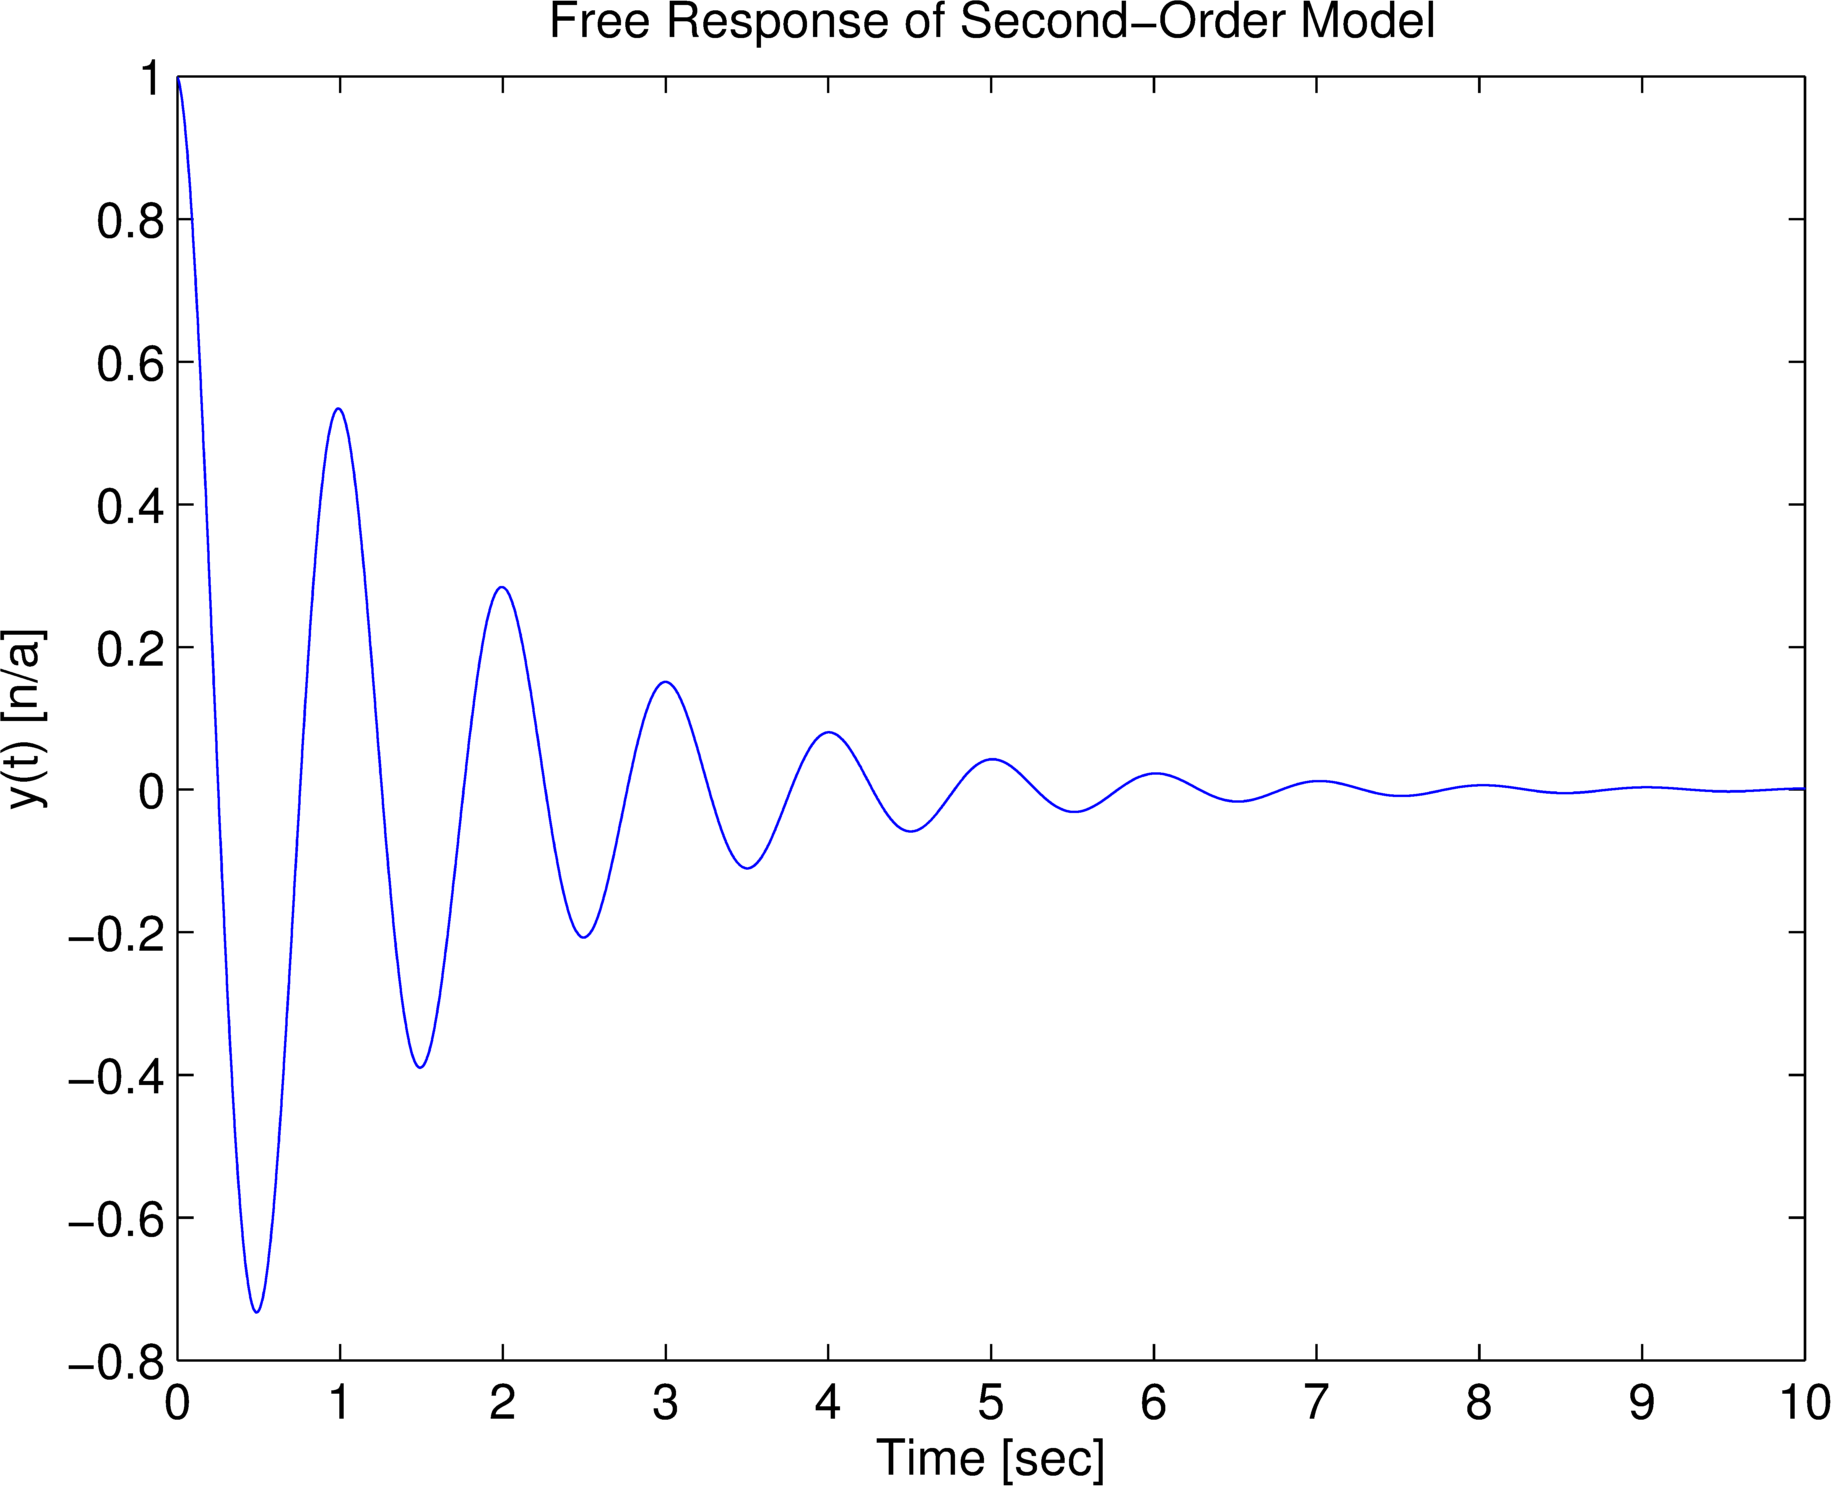
\includegraphics[width=\FigWidth\textwidth]{second_free.png}
\caption{Graph of the free response (\ref{e:stepresp}) with $\omega_n= \unit[1]{Hz}$, $\zeta=0.1$ (10\%) and $y(t=0)=1$.}
\label{f:secondfree}
\end{figure}

\begin{ex}
There is a mistake in Listing~\ref{l:secondfree} which attempted to display the solution for the case where there is only a ``displacement'' initial condition: i.e., $y(0)=y_o$ and $\dot{y}(0)=0$.  The mistake is that the solution in the code uses the values $C=y_o$ and $\phi=0$ which are not correct (but they are close). 
\begin{itemize}\label{ex:secondresp}
\item Derive expressions for the constants $C$ and $\phi$ based on the initial conditions $y(0)=y_o$ and $\dot{y}(0)=0$.
\item Copy the script in Listing~\ref{l:secondfree} and create the graph shown in Figure~\ref{f:secondfree}.
\item Correct the script in Listing~\ref{l:secondfree} and plot a second curve, on the same axes, with the corrected solution for $y_o=1$.  
  \begin{itemize}
  \item Include your MATLAB script with your solution.
  \item Include your graph as a properly formatted figure.
  \end{itemize}
\end{itemize}
The error is simply in the calculation of $C$ and $\phi$; the structure of the script in Listing~\ref{l:secondfree} should work just fine.
\end{ex}

\ifsolutions
\begin{soln}
\[ C = \sqrt{\frac{y_o}{1-\zeta^2}} \]
\[ \tan\phi = \frac{\zeta}{\sqrt{1-\zeta^2}} \]
or 
\[ \phi = \arctan\left(\frac{\zeta}{\sqrt{1-\zeta^2}}\right) \]

See Figure~\ref{f:secondfreesoln}.  This figure is generated using Listing~\ref{l:seconfree2}

\lstinputlisting[style=myMatStyle,
caption={Script for plotting the corrected free response of a second-order model.},
label={l:secondfree2}]
{../code/soln/second_order_free_correct.m}

\begin{figure}[hbt]
\centering
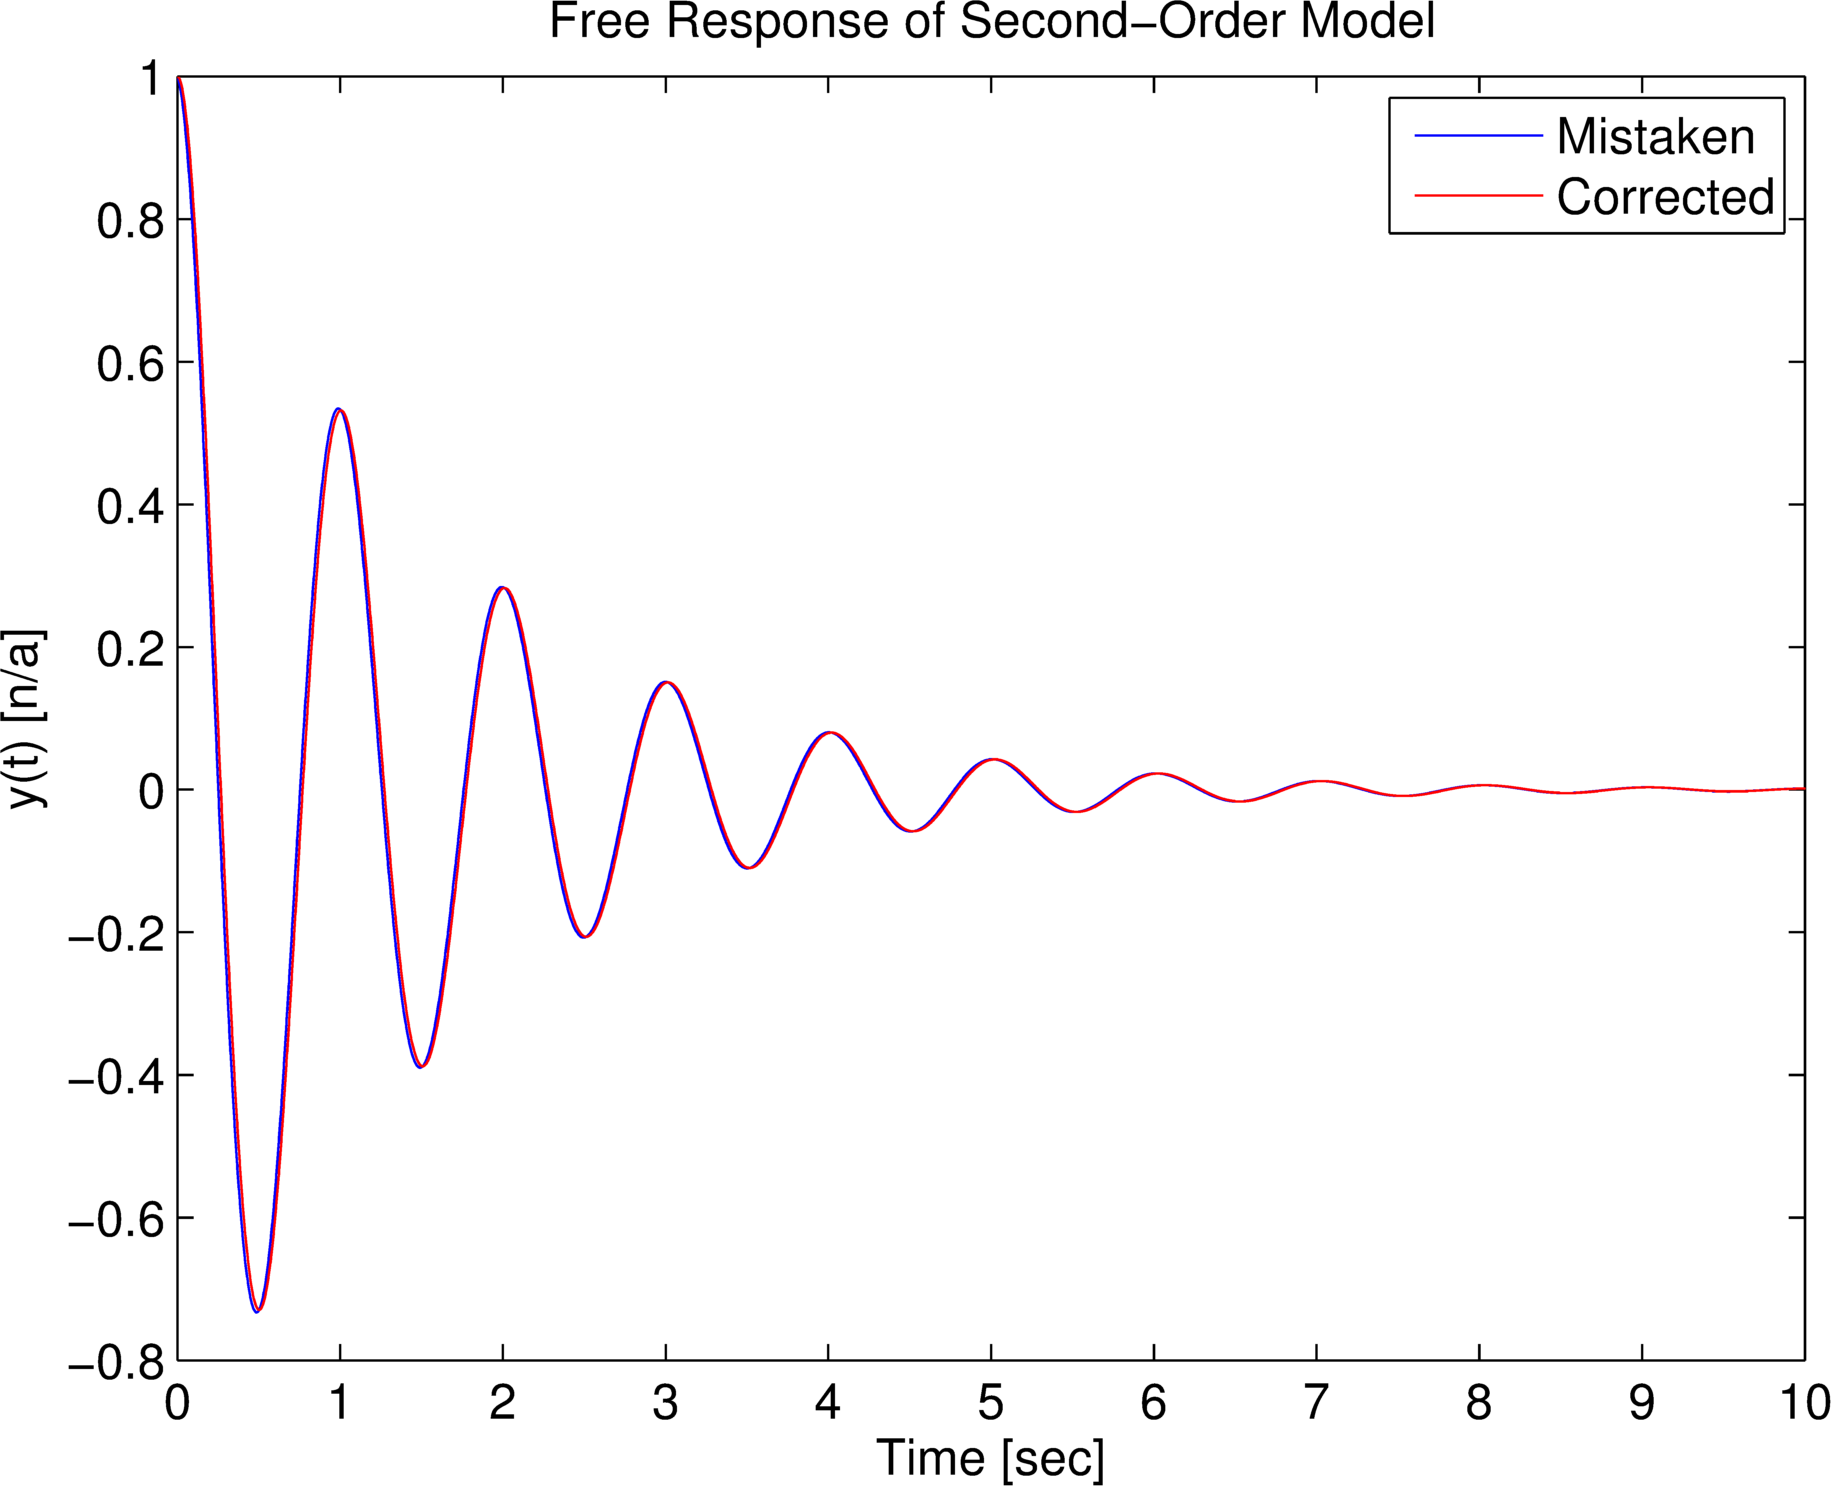
\includegraphics[width=\FigWidth\textwidth]{second_free_soln.png}
\caption{Graphs of the original mistaken free response and the corrected free response.}
\label{f:secondfreesoln}
\end{figure}
\end{soln}
\fi

\begin{ex}
Consider the effect of the damping ratio ($\zeta$) on the shape of free response.  Using Listing~\ref{l:secondfree} as a starting point, use MATLAB to create a single graph for the free response with the initial conditions $y(0)=1$ and $\dot{y}(0)=0$.  On a single set of axes, plot the response for systems with the following values for the damping ratio: $\zeta=\{0.0, 0.01 , 0.1, 0.5, 0.9\}$.  Use a legend to declare which curve is associated with each value of $\zeta$.  Submit this single graph as an appropriately formatted figure with a short description of what you observe about the effect of changing $\zeta$.
\end{ex}

\ifsolutions
\begin{soln}
See Figure~\ref{f:secondfreezetas} generated using Listing~\ref{l:secondfreezeta}.

\lstinputlisting[style=myMatStyle,
caption={Script for plotting the free response of a second-order model with varios values of zeta.},
label={l:secondfreezeta}]
{../code/second_order_free_zeta.m}


\begin{figure}[hbt]
\centering
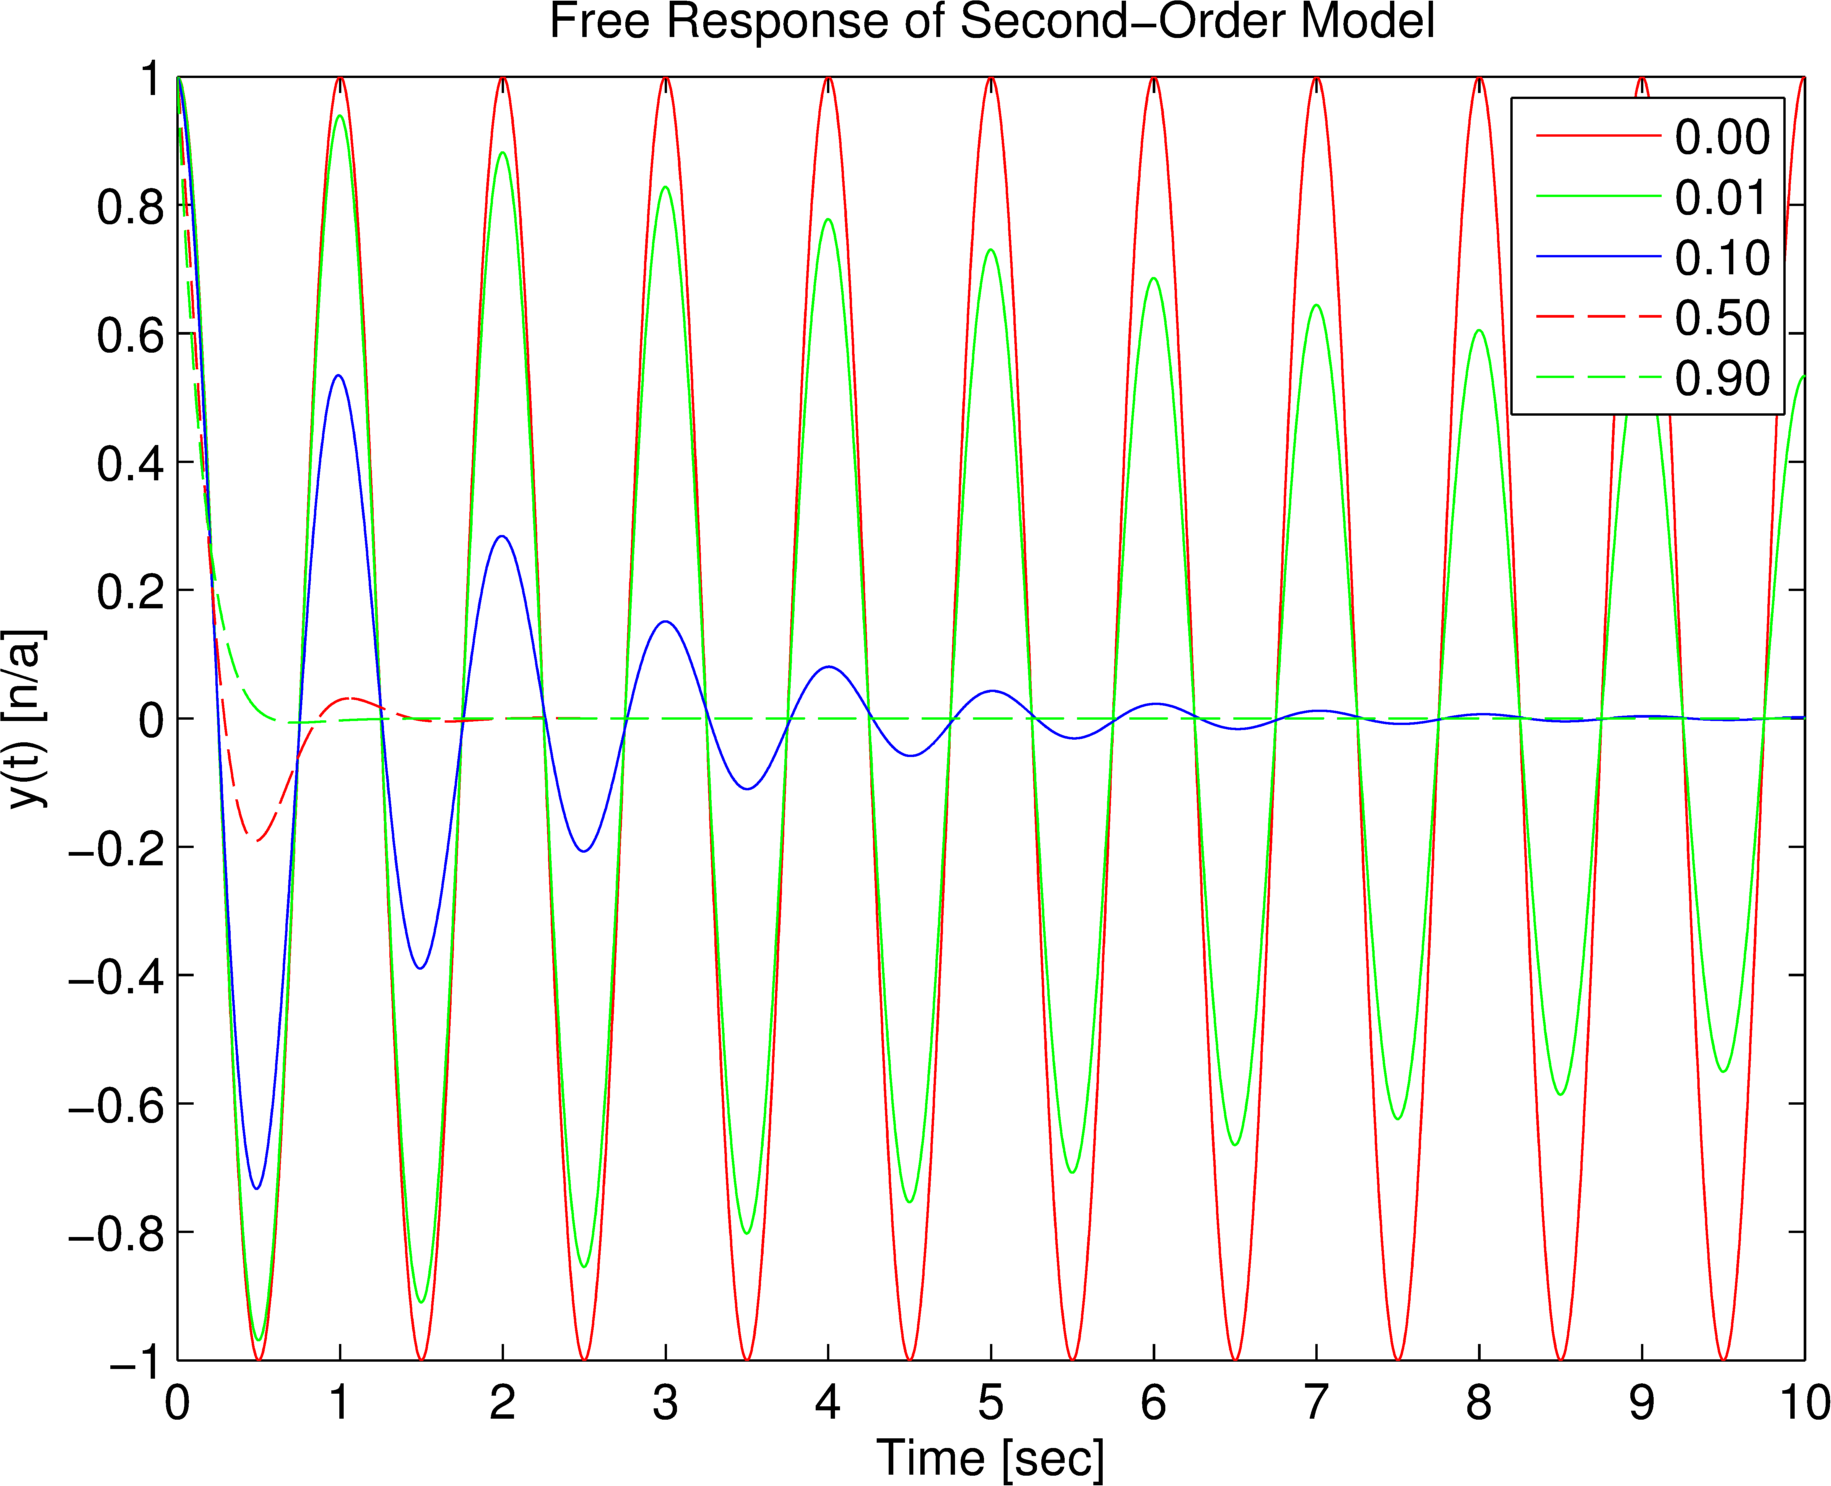
\includegraphics[width=\FigWidth\textwidth]{free_zetas.png}
\caption{}
\label{f:secondfreezetas}
\end{figure}

\end{soln}
\fi

\begin{ex}
Consider the model's free response to velocity-only initial conditions---$y(0)=0$ and $\dot{y}(0)=v_o$.
\begin{itemize}
\item Derive expressions for the constants $C$ and $\phi$ based on these initial conditions.
\item Substitute your expressions into the response (\ref{e:secondfree}) and write a simplified equation for the response.  (Hint: $\cos\left(u-\frac{\pi}{2}\right) = \sin(u)$.)
\item Using MATLAB, create a figure the graphs the response ($y(t)$) to this initial condition.
\end{itemize}
\end{ex}


\begin{ex}
Given a damping ratio of $\zeta=0.01$ (1\% damping), write and expression for the damped natural frequency as a function of the undamped natural frequency.  \\
Repeat the exercise for a 10\% damping.
\end{ex}




\section{Example: Cantilevered Beam}
Another physical system that has a response that can be approximated by our second-order model is a cantilevered beam.  Imagine a yardstick fixed on one end.  When the free end is subject to a displacement (the initial condition) and then released, the tip will oscillate.  A cantilevered beam, unlike our lumped mass system in Figure~\ref{f:msd2}, is a continuous system, but for now we'll approximate it by examining the first natural frequency.  

\subsection{First-Mode of Cantilevered Beam}
The first natural frequency of a uniform cantilevered beam, Figure~\ref{f:blevins}, can be estimated by using classical beam theory.
\begin{figure}[htb!]
\centerline{
{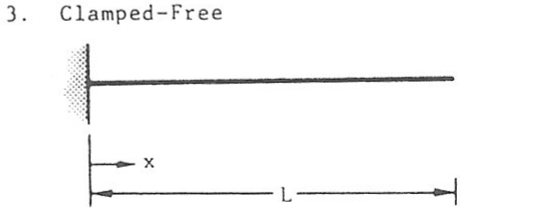
\includegraphics[width=0.4\textwidth]{blevins_beam.png}}}
\caption{Image of a cantilevered beam model.  From ``Formulas for Natural Frequency and Mode Shape'' by R. D. Blevins.}
\label{f:blevins}
\end{figure}
The resulting expression for the first natural frequency, in \unitfrac[]{rad}{s}, is
\begin{equation}\label{e:blevins}
\omega_n = \frac{(1.875)^2}{L^2} \sqrt{\left( \frac{EI}{\rho} \right)}
\end{equation}
where $\rho$ is the mass per unit length of the beam (the product of the density and the cross-section area), $E$ is the modulus of elasticity of the beam material, $I$ is the second moment of area of the beam and $L$ is the length of the beam. 

\subsection{First-Mode of Cantilevered Beam with Added Mass}
Similarly, it is possible to predict the natural frequency of a uniform cantilevered beam with a point-mass at the free end of the beam as illustrated in Figure~\ref{f:blevinsmass}.
\begin{figure}[htb!]
\centerline{
{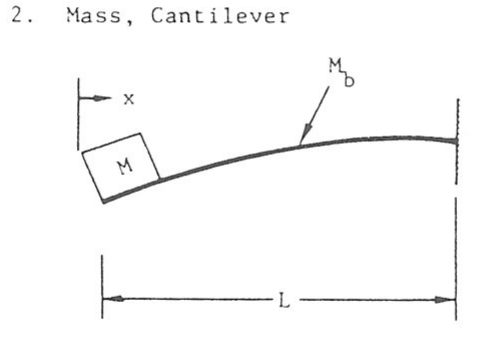
\includegraphics[width=0.4\textwidth]{blevins_beam_mass.png}}}
\caption{Image of a cantilevered beam with point mass model from ``Formulas for Natural Frequency and Mode Shape'' by R. D. Blevins.}
\label{f:blevinsmass}
\end{figure}
The first natural frequency for this model is
\begin{equation}\label{e:blevinsmass}
\omega_n = \sqrt{ \frac{3 E I}{L^3 (M+0.24 M_b)}}
\end{equation}
where $M$ is the point mass at the free end of the beam and $M_b$ is the total mass of the beam.

Notice that both predicted natural frequencies (\ref{e:blevins}) and (\ref{e:blevinsmass}) have the general from of $\omega_n = \sqrt{K/M}$ where $K$ is the ``stiffness'' of the system and $M$ is the ``mass'' of the system.


\begin{ex}\label{ex:beamvib}
Given a uniform cantilevered beam with the following properties:
\begin{itemize}
\item Length = \unit[0.5]{m}
\item Width = \unit[2.54]{cm}
\item Thickness = \unit[1.59]{mm}
\item Modulus of Elasticity ($E$) = \unit[68.9]{GPa}
\item Density = \unitfrac[2.70]{g}{cm$^3$}
\end{itemize}
Predict the undamped natural frequency.  Express the answer in both of the following units: \unitfrac[]{rad}{s} and \unit[]{Hz}.
\end{ex}

\ifsolutions
\begin{soln}
Use (\ref{e:blevins}) with the values from the Exercise.  The mass-per-unit-length is the product of the density and the cross-sectional area:
\[ \rho = D*(t*W) \]
where $D$ is the density, $t$ is the beam thickness and $W$ is the beam width.
We also need to calculate the second moment of area...
\[ I = 1/12(W*t^3) \]
If we plug in these values we get...
\[ \omega_n = \unitfrac[32.6]{rad}{s} \]
To express in Hz
\[ f_n = \frac{\unitfrac[\omega_n]{rad}{s}}{\unitfrac[2\pi]{rad}{cycle}} = \unitfrac[5.2]{cycles}{s}=\unit[5.2]{Hz}
\]

\lstinputlisting[style=myMatStyle,
caption={Script for predicting the natural frequency of a cantilevered beam.},
label={l:natlfreq}]
{../code/natl_freq_pred.m}

\end{soln}
\fi

\begin{ex}\label{ex:model2sim}
Given the uniform cantilevered beam described in the previous example, and a damping ratio of $\zeta=0.02$ (2\% damping)...
\begin{itemize}
\item Write an expression for a mathematical model of the form in (\ref{e:second}) to describe the system.  (You should just need to substitute in numerical values for the system parameters $\zeta$ and $\omega_n$.)
\item Using MATLAB, produce a graph that predicts the response of the tip of the cantilevered beam to an initial displacement of \unit[1.0]{cm} and zero initial velocity: $y(0)=\unit[1.0]{cm}$ and $\dot{y}(0) = \unitfrac[0]{cm}{s}$.
\end{itemize}
\end{ex}

\ifsolutions
\begin{soln}
\[
\ddot{y}(t) + 2 (0.02) (32.6)\dot{y}(t) + (32.6)^2 = f(t)
\]
To generate the graph we can use the same script from Exercise~\ref{ex:secondresp} and substitute in the new values for $\zeta$ and $\omega_n$.

\lstinputlisting[style=myMatStyle,
caption={Script for plotting the corrected free response of a second-order model using the given beam parameters.},
label={l:secondfreemodelsoln}]
{../code/second_order_free_model.m}

\begin{figure}[hbt]
\centering
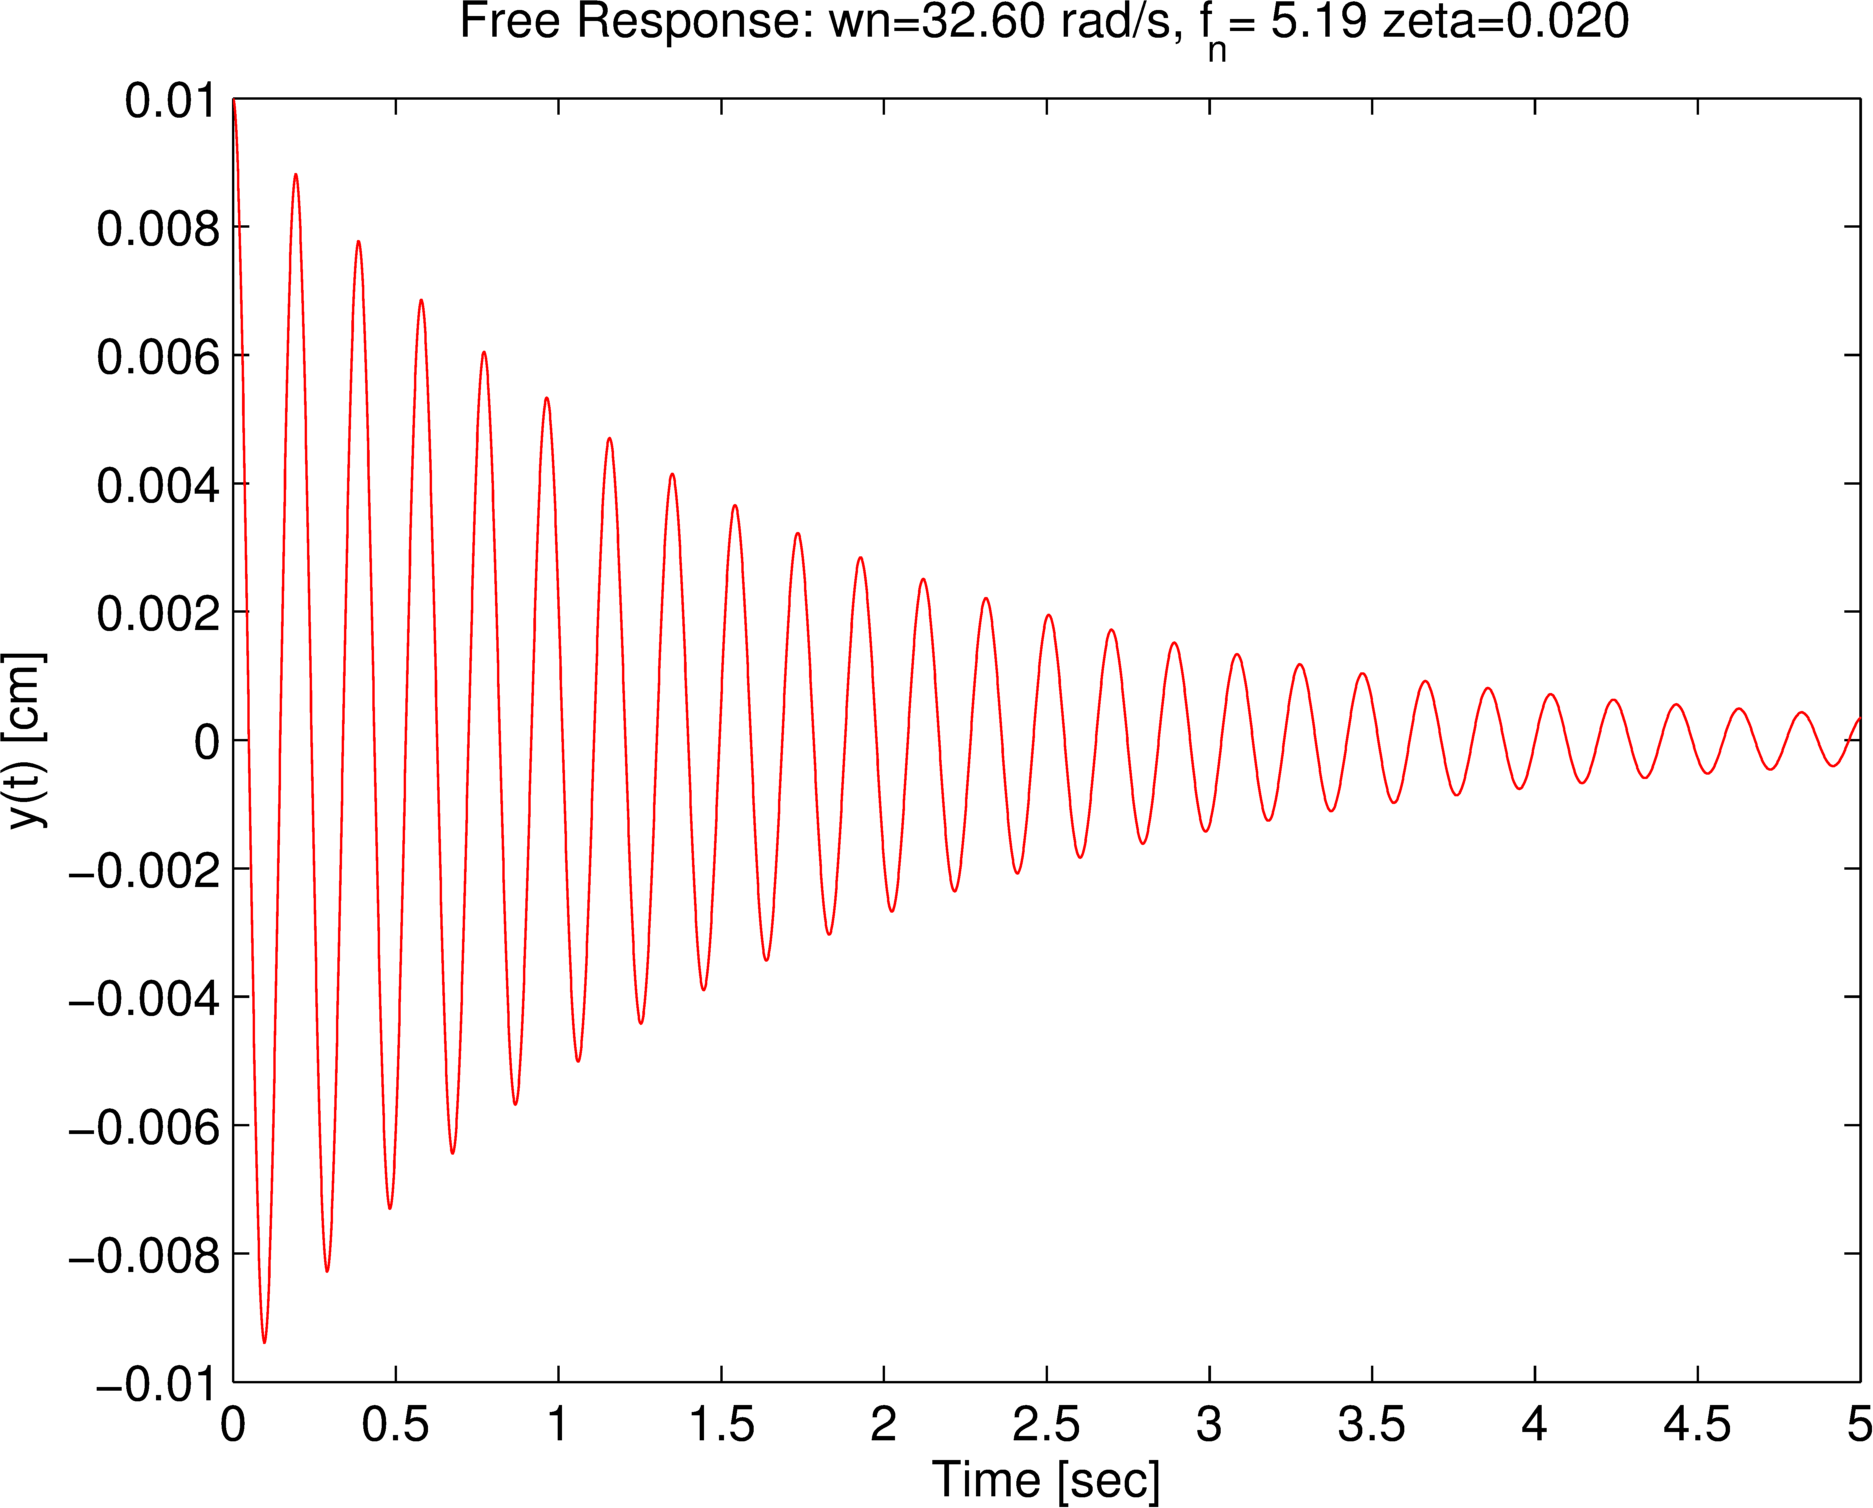
\includegraphics[width=\FigWidth\textwidth]{soln_second_free_model.png}
\caption{Graphs of the second-order free response for the predicted natural frequency from the given beam parameters.}
\label{f:soln2freemodel}
\end{figure}

\end{soln}
\fi


\section{Measuring Second-Order Response}
For physical systems that exhibit oscillatory response we can ``fit'' a second-order response to the system measurements to estimate the system parameters ($\omega_n$ and $\zeta$) based on the measured response.  In other words, consider that you measure the time response of a system (e.g., a cantilevered beam, a RLC circuit, etc.) and you observe that the behavior looks something like Figure~\ref{f:secondfreeresp}.  How can you estimate the natural frequency and damping ratio associated with such a response?

\begin{figure}[h!bt]
\centerline{
{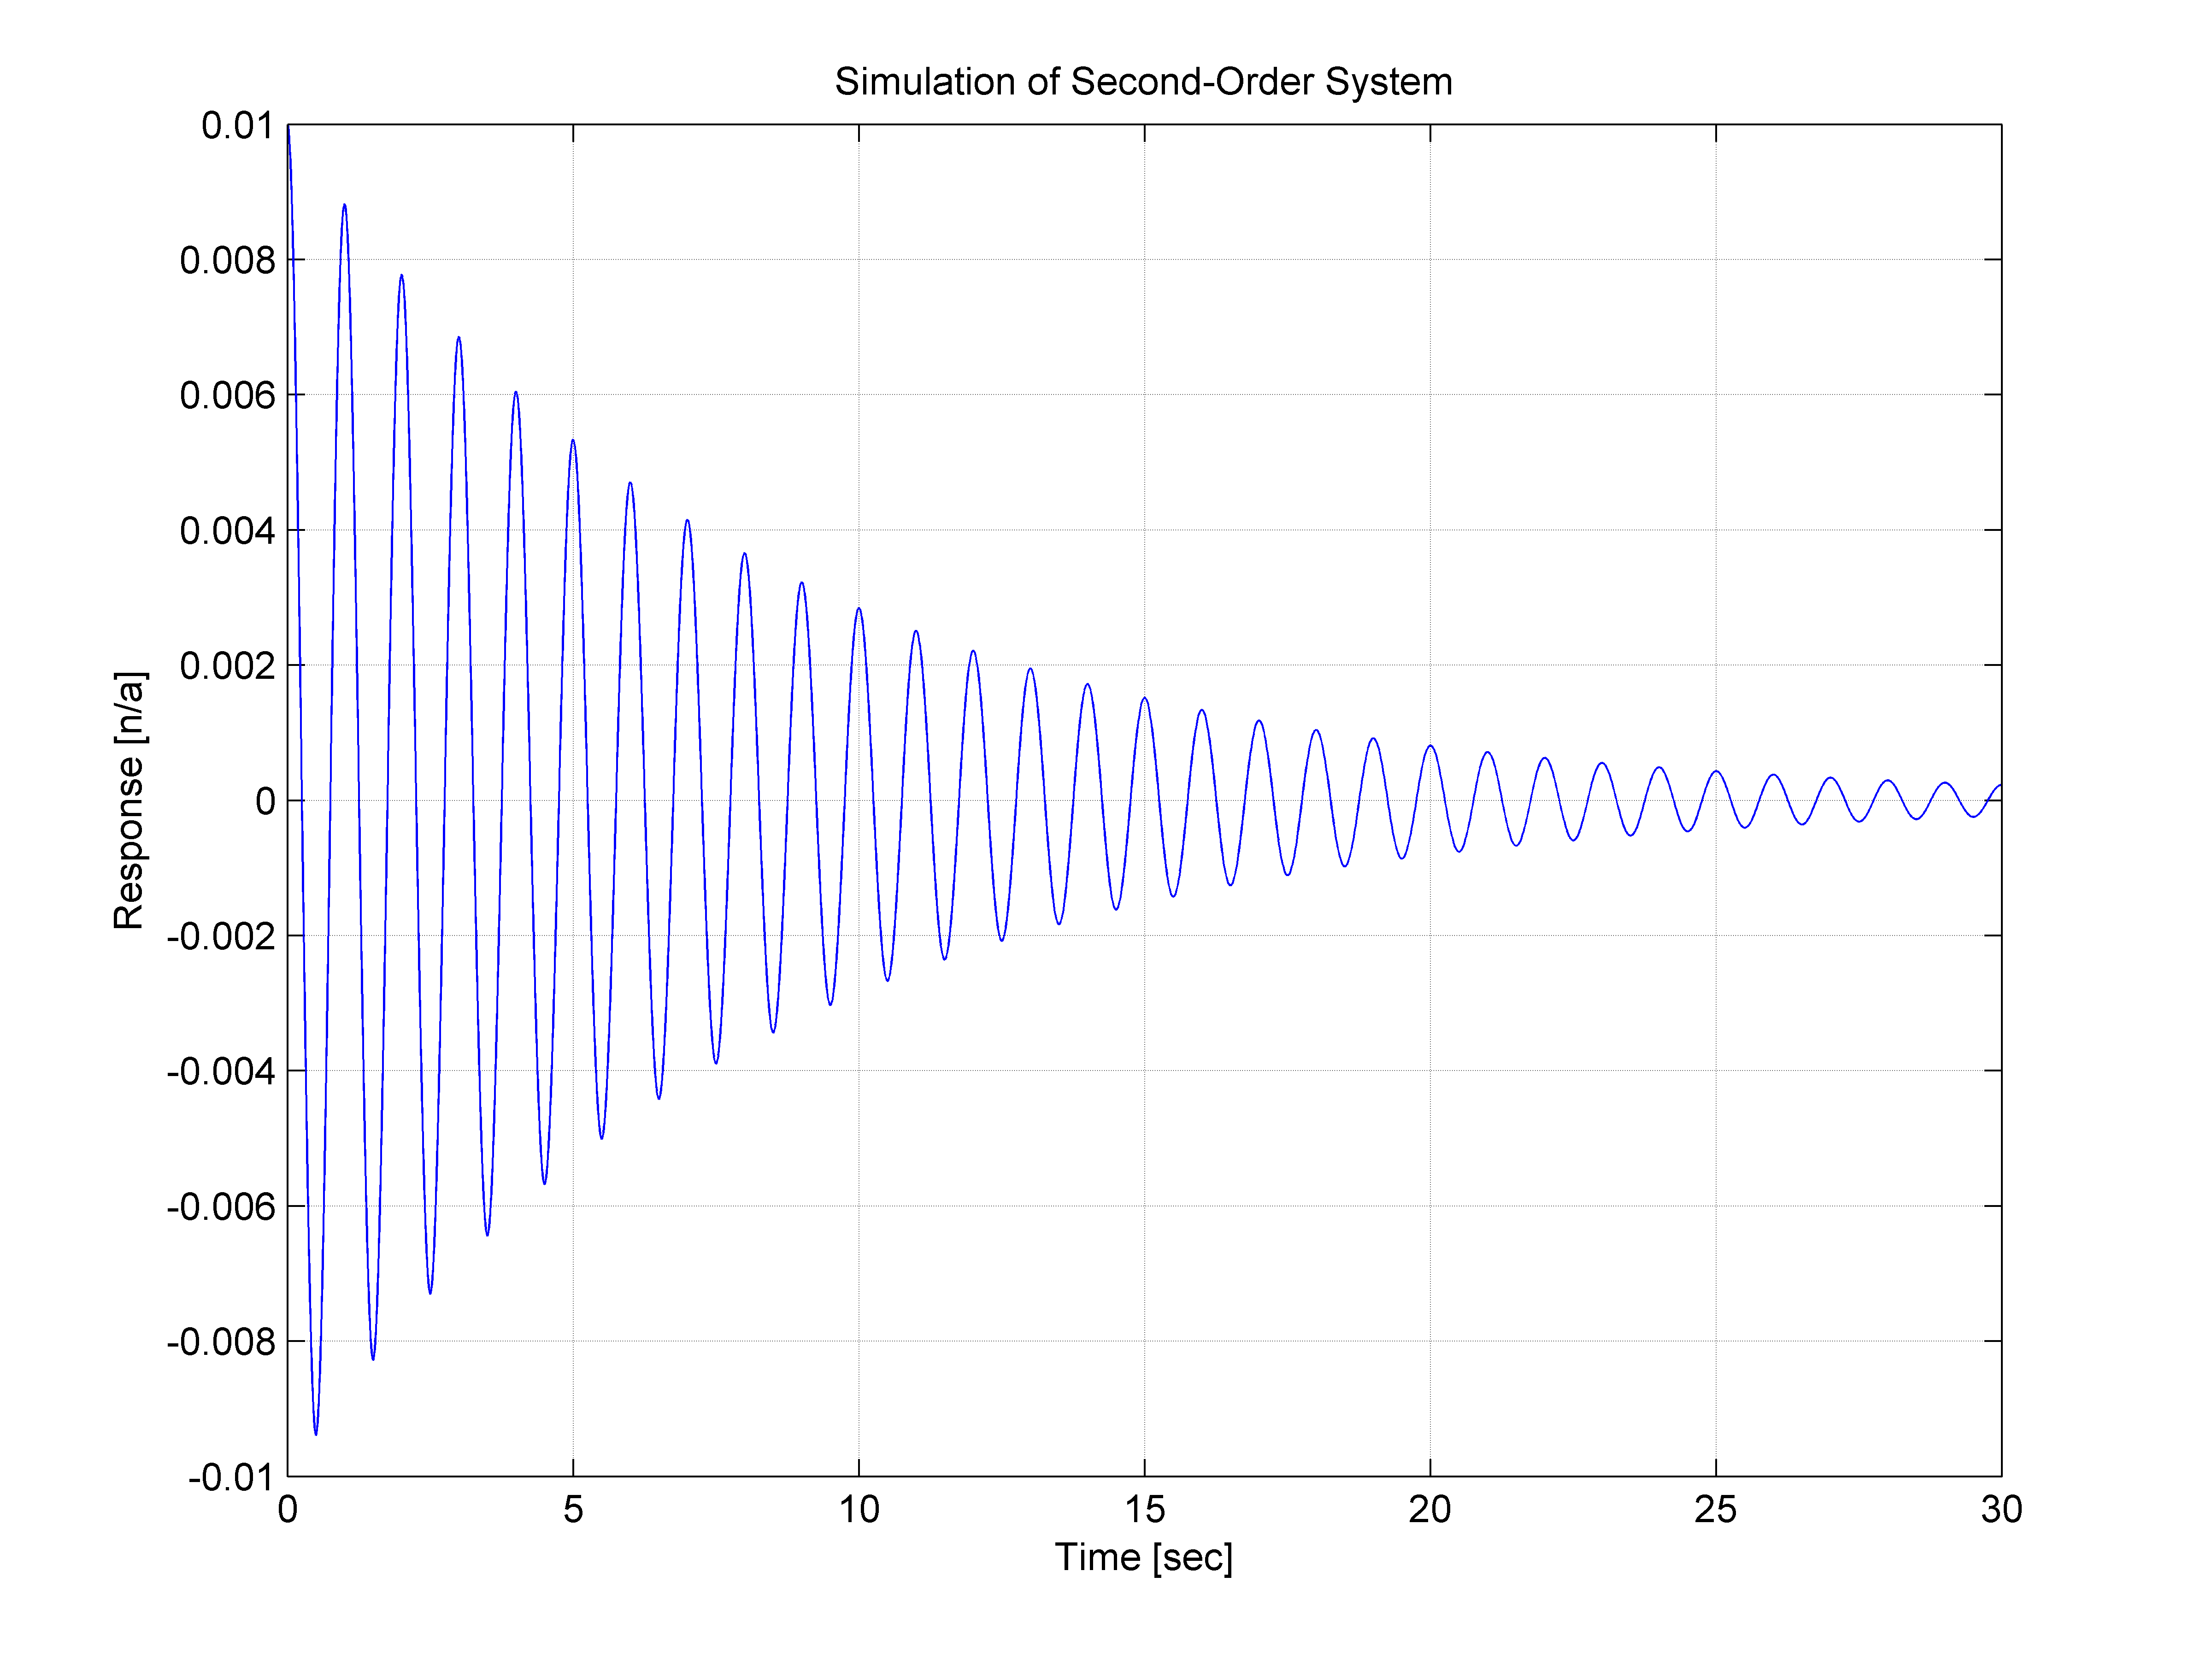
\includegraphics[width=0.6\textwidth]{second_order_grid.png}}}
\caption{Illustration of the free-response of a second-order system.  The response shows the analytical solution for $y(t)$.}
\label{f:secondfreeresp}
\end{figure}

\subsection{Measuring Frequency}
It may be obvious, but if for no other reason than to get the units (\unit[]{Hz} and \unitfrac[]{rad}{s}) it is worth spending a little time discussing how to measure the frequency of oscillation from a measured response.  Since our measurements are of the {\bf time} response, we will need to start by estimating the period of oscillation, the time it takes for one cycle of oscillation.  We could do this by measuring the time between two adjacent peaks in the response, but a better way is to measure the elapsed time ($\Delta t$) between two peaks (or troughs, or zero-crossings) of the response and the number of cycles ($n$) as illustrated in Figure~\ref{f:secondtime}.
\begin{figure}[h!bt]
\centerline{
{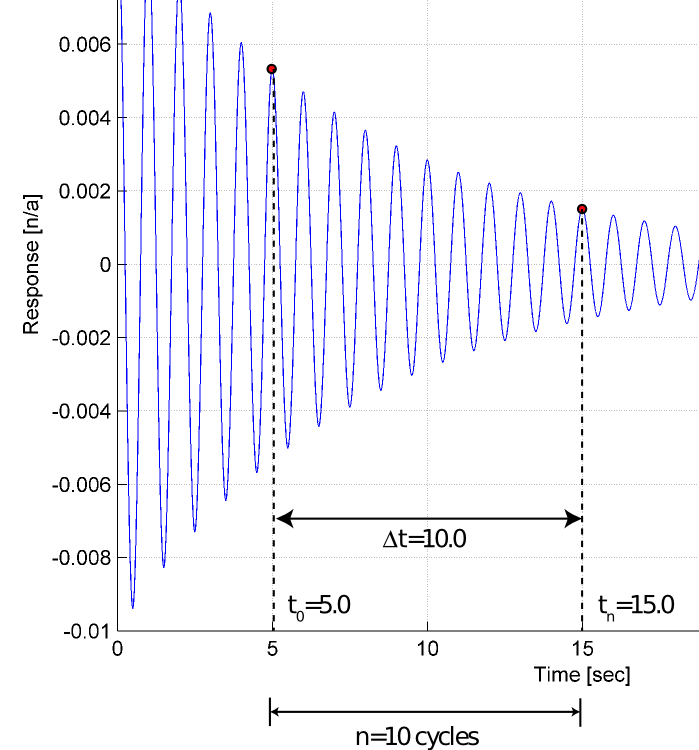
\includegraphics[width=0.6\textwidth]{second_order_grid_time_only_annote_crop.png}}}
\caption{Illustration of measuring the period of oscillation.}
\label{f:secondtime}
\end{figure}
Then we can estimate the average period of oscillation as
\begin{equation}
T = \frac{t_n-t_o}{n}=\frac{\Delta t}{n}=\frac{\unit[10.0]{s}}{\unit[10]{cycles}} = \unitfrac[1.0]{s}{cycle}.
\end{equation}
The corresponding frequency of oscillation ($f_d$ (in Hz)) is the reciprocal of the period
\begin{equation}
f_d = \frac{1}{T} = \frac{1}{\unitfrac[1.0]{s}{cycle}} = \unitfrac[1.0]{cycles}{s} = \unit[1.0]{Hz}.
\end{equation}
The last step is to convert the units of this frequency from Hz to \unitfrac[]{rad}{s} with the expression
\begin{equation}
\omega_d = f_d (2 \pi) = \unitfrac[1.0]{cycles}{s} (\unitfrac[2 \pi]{rad}{cycle}) = \unitfrac[6.28]{rad}{s}.
\end{equation}
It is important to notice that what we have estimated here is the {\bf damped} natural frequency ($\omega_d$), not the undamped natural frequency ($\omega_n$).  Again, the relationship between these two quantities is
\begin{equation}
\omega_n = \frac{\omega_d}{\sqrt{1-\zeta^2}}.
\end{equation}
To estimate $\omega_n$ we'll need to know (to estimate) the damping ratio ($\zeta$).

\subsection{Measuring the Damping Ratio Via Logarithmic Decrement Method}

The logarithmic decrement method is a technique to empirically identify the damping ratio ($\zeta$) of a second-order underdamped model.  The method is based on the characteristic time response of the model.  The time response can be either the response to a step input or the free-response to a non-zero initial condition.  The free-response to an initial condition is given in your textbook as
\begin{equation}
y_h(t)=C e^{-\zeta\omega_nt}\sin\left(\omega_dt+\phi\right) 
\end{equation}
where $\omega_n$ is the undamped natural frequency of the system and $\omega_d=\omega_n\sqrt{1-\zeta^2}$ is the damped natural frequency.  The two constants $C$ and $\phi$ are determined from the initial conditions.

To estimate the damping ratio can be estimated in the following way.  First plot the response $y(t)$ as a function of time.  Choose two peaks of the oscillatory response $y_0$ and $y_n$ where $y_0$ is the larger value that happens earlier in time.  Calculate the logarithmic decrement ($\delta$) as
\[ \delta = \frac{1}{n}\ln\left(\frac{y_0}{y_n}\right) \]
where $n$ is the number of cycles between $y_0$ and $y_n$.
Finally calculate the damping ratio as
\[ \zeta = \frac{1}{\sqrt{1+\left(\frac{2\pi}{\delta}\right)^2}}. \]

\subsubsection{Example}
Figure \ref{f:secondfreeresp} illustrates the free response of a second-order model to an initial condition of $y(0)=0.01$ and $\dot{y}(0)=0$.  The undamped natural frequency is \unitfrac[$2 \pi$]{rad}{s}.

To calculate the logarithmic decrement we need to select two peaks from the response as shown in Figure~\ref{f:resp2}\footnote{The MATLAB function \texttt{ginput()} is handy for selecting the values from a figure window.}. These selected values, along with the equations above, result in $\delta=0.124$ and $\zeta=0.0198$.  This estimate is quite close to the value of 0.02 which was used to generate the example.

\begin{figure}[h!bt]
\centerline{
{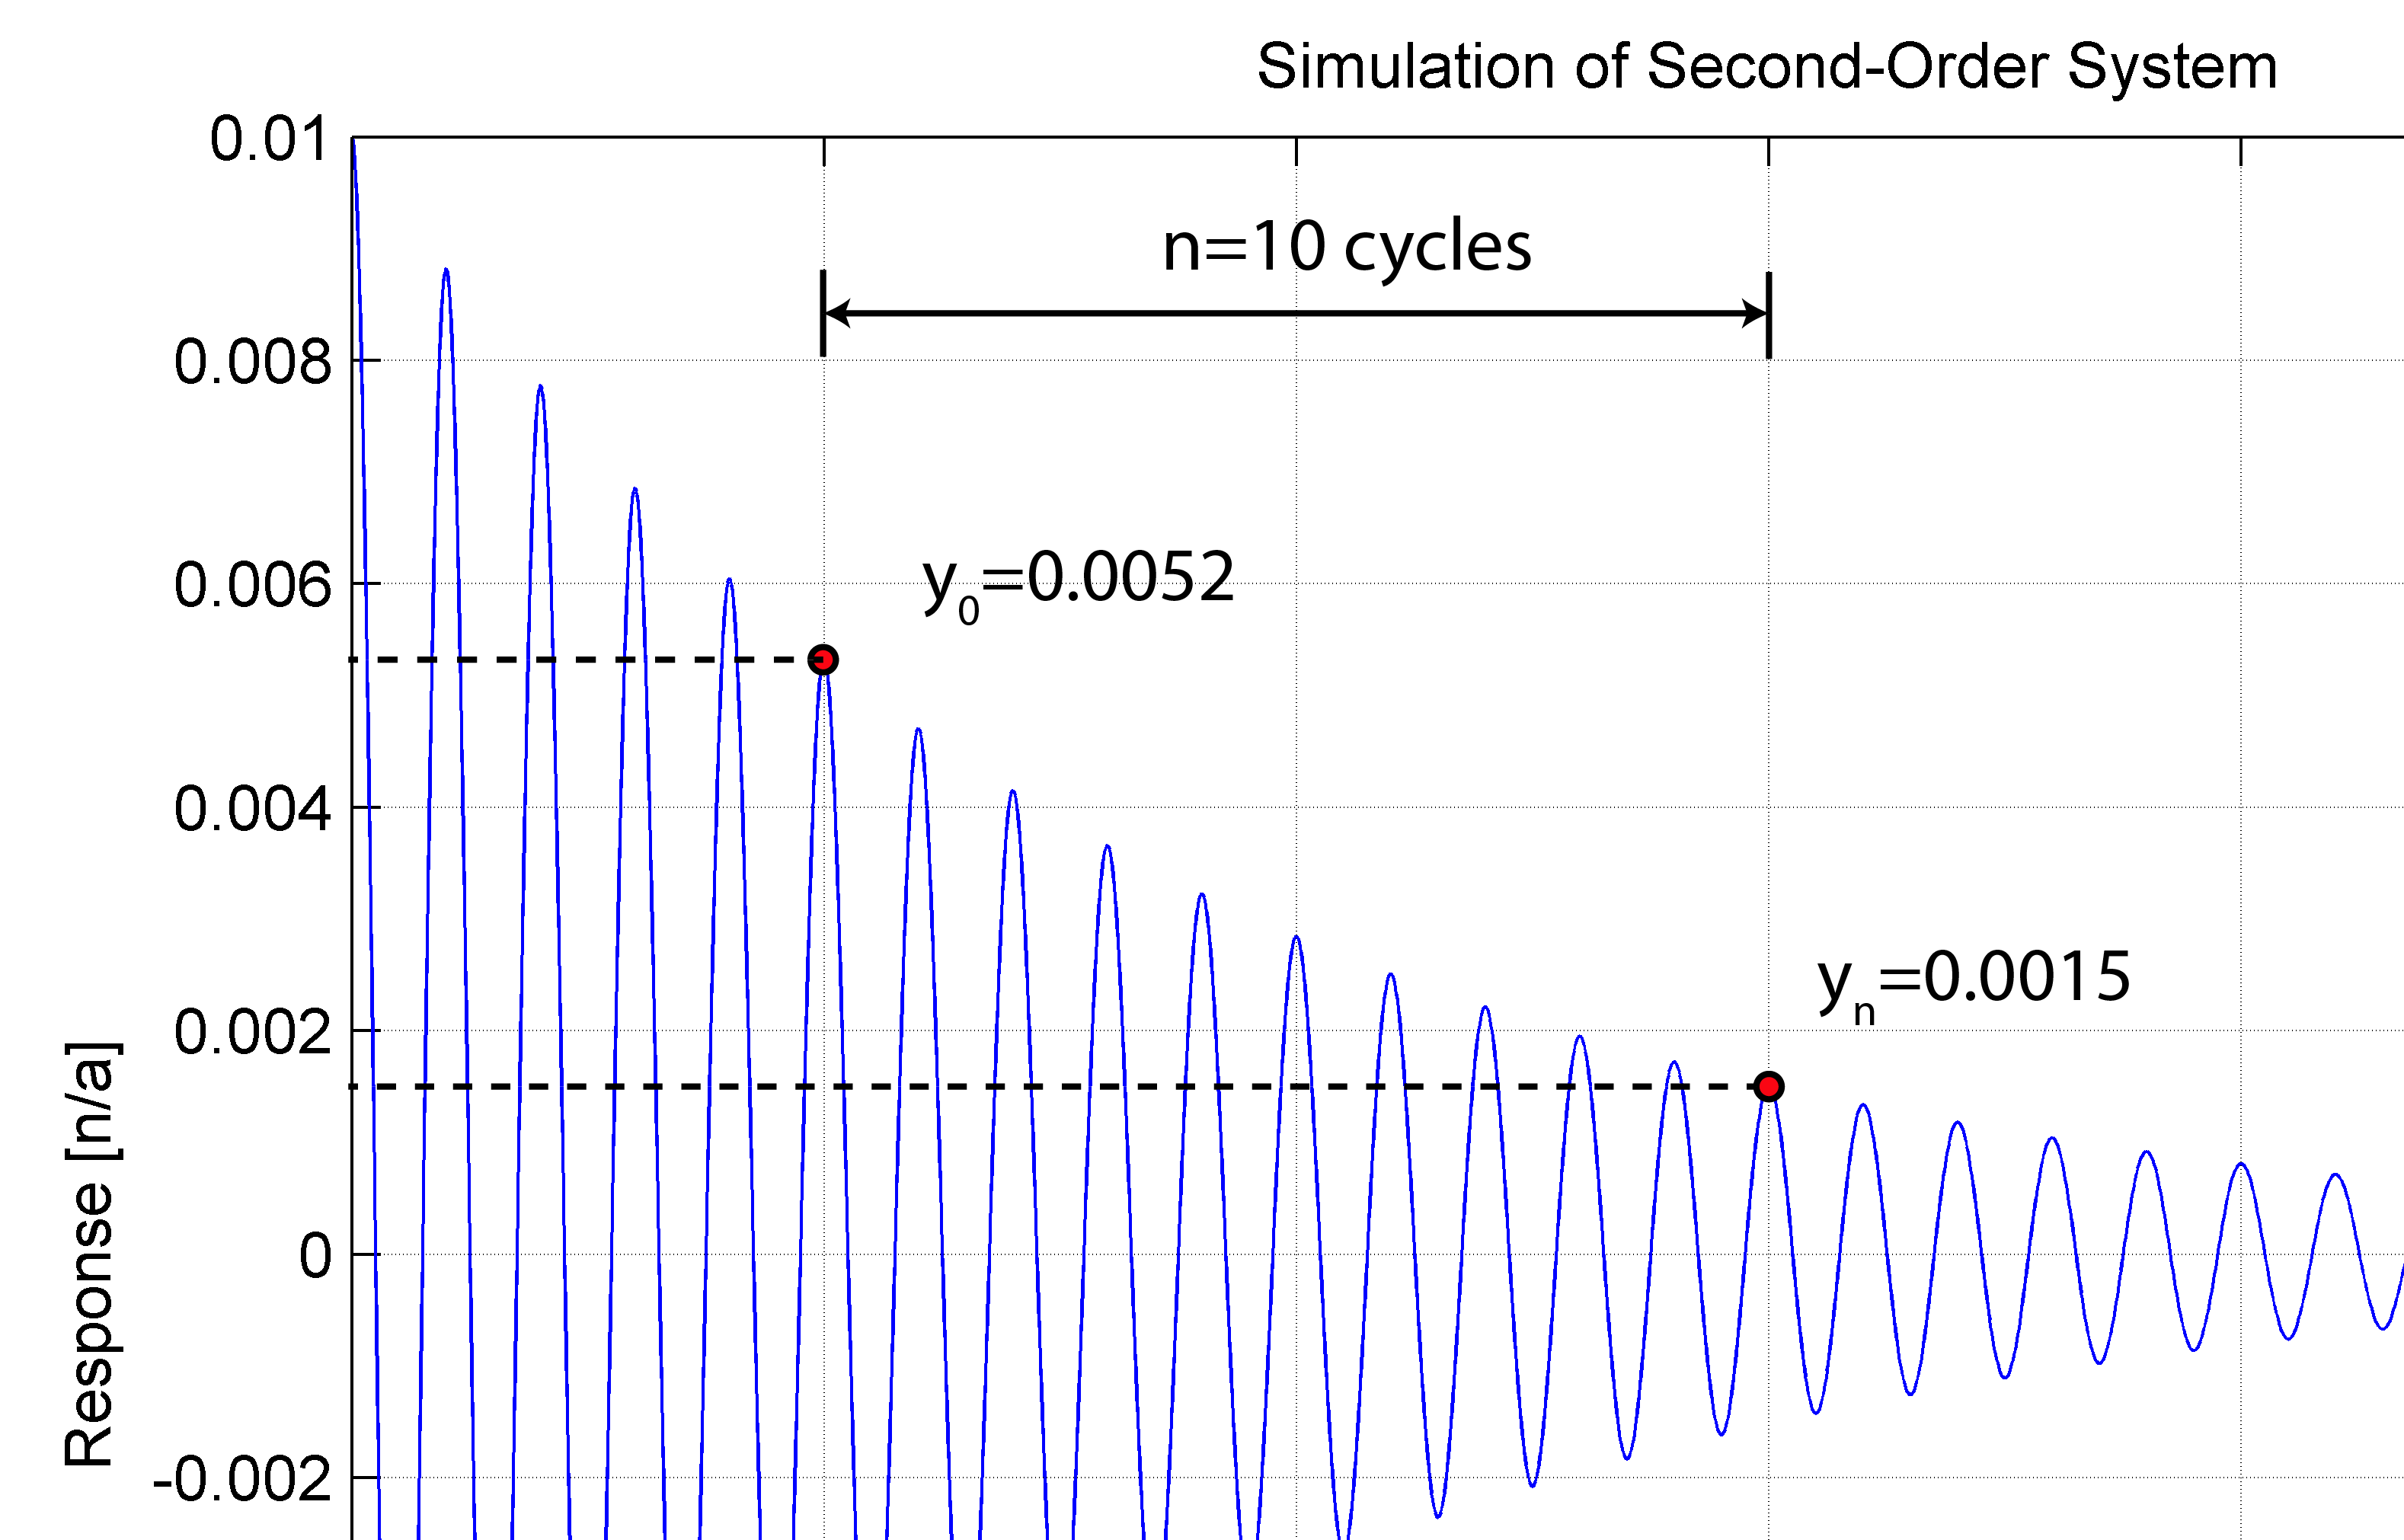
\includegraphics[width=0.6\textwidth]{second_order_grid_annote_crop.png}}}
\caption{The added annotation illustrates the selection of ``peaks'' in the response to initiate the logarithmic decrement process.}
\label{f:resp2}
\end{figure}

%\afterpage{\clearpage}

\subsubsection{Why It Works}
The logarithmic decrement method is based on fitting a curve to the data.  In this case the curve (the model) is the exponential amplitude of the second-order response
\begin{equation}
y_{env}(t)=C e^{-\zeta\omega_nt}.
\label{e:env}
\end{equation}
This function is superimposed on the response in Figure~\ref{f:env}.
\begin{figure}[h!bt]
\centerline{
{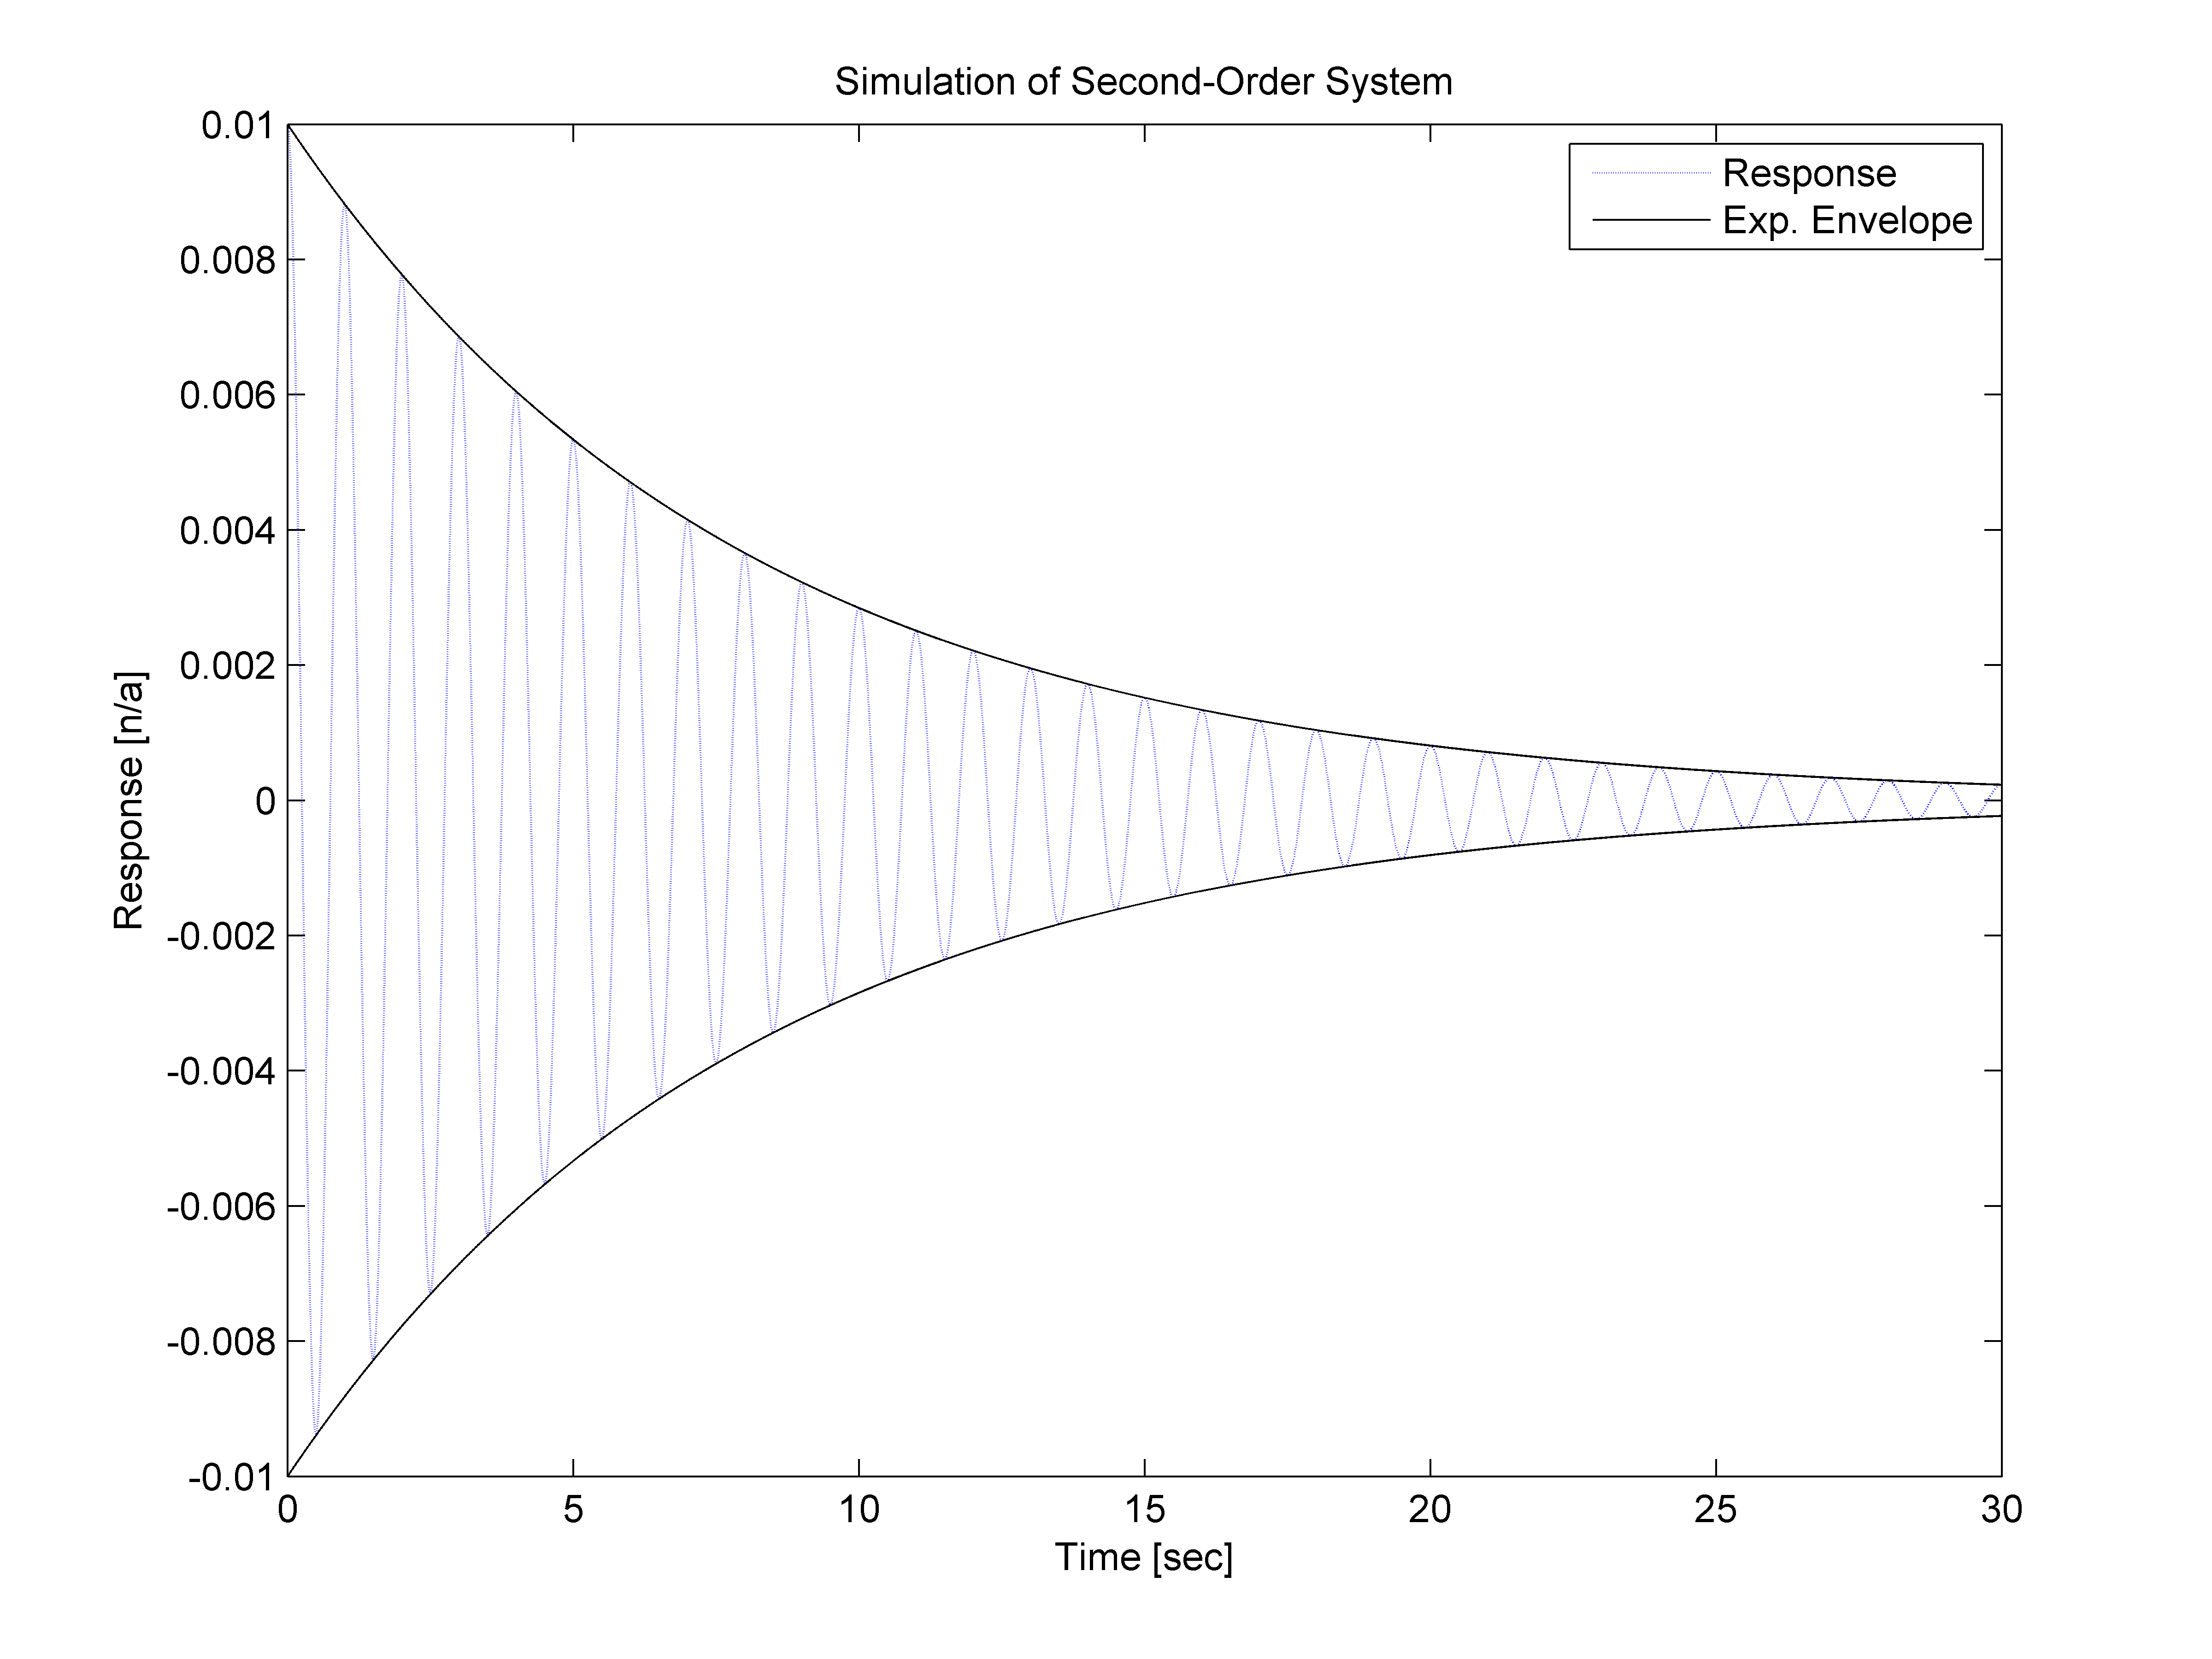
\includegraphics[width=0.6\textwidth]{second_order_env.png}}}
\caption{Second-order free response with the exponential envelope function included (\ref{e:env})}.
\label{f:env}
\end{figure}

If we take the natural logarithm of this function we get a linear relationship between $Y_{ln}=\ln(y_{env})$ and $t$:
\[
Y_{ln}=\ln(y_{env})=(-\zeta \omega_n) t.
\]
This linear relationship is illustrated in Figure~\ref{f:ln} where $Y_{ln}$ is plotted versus time.  The slope of the line is $m=-\zeta \omega_n$.
\begin{figure}[hbt!]
\centerline{
{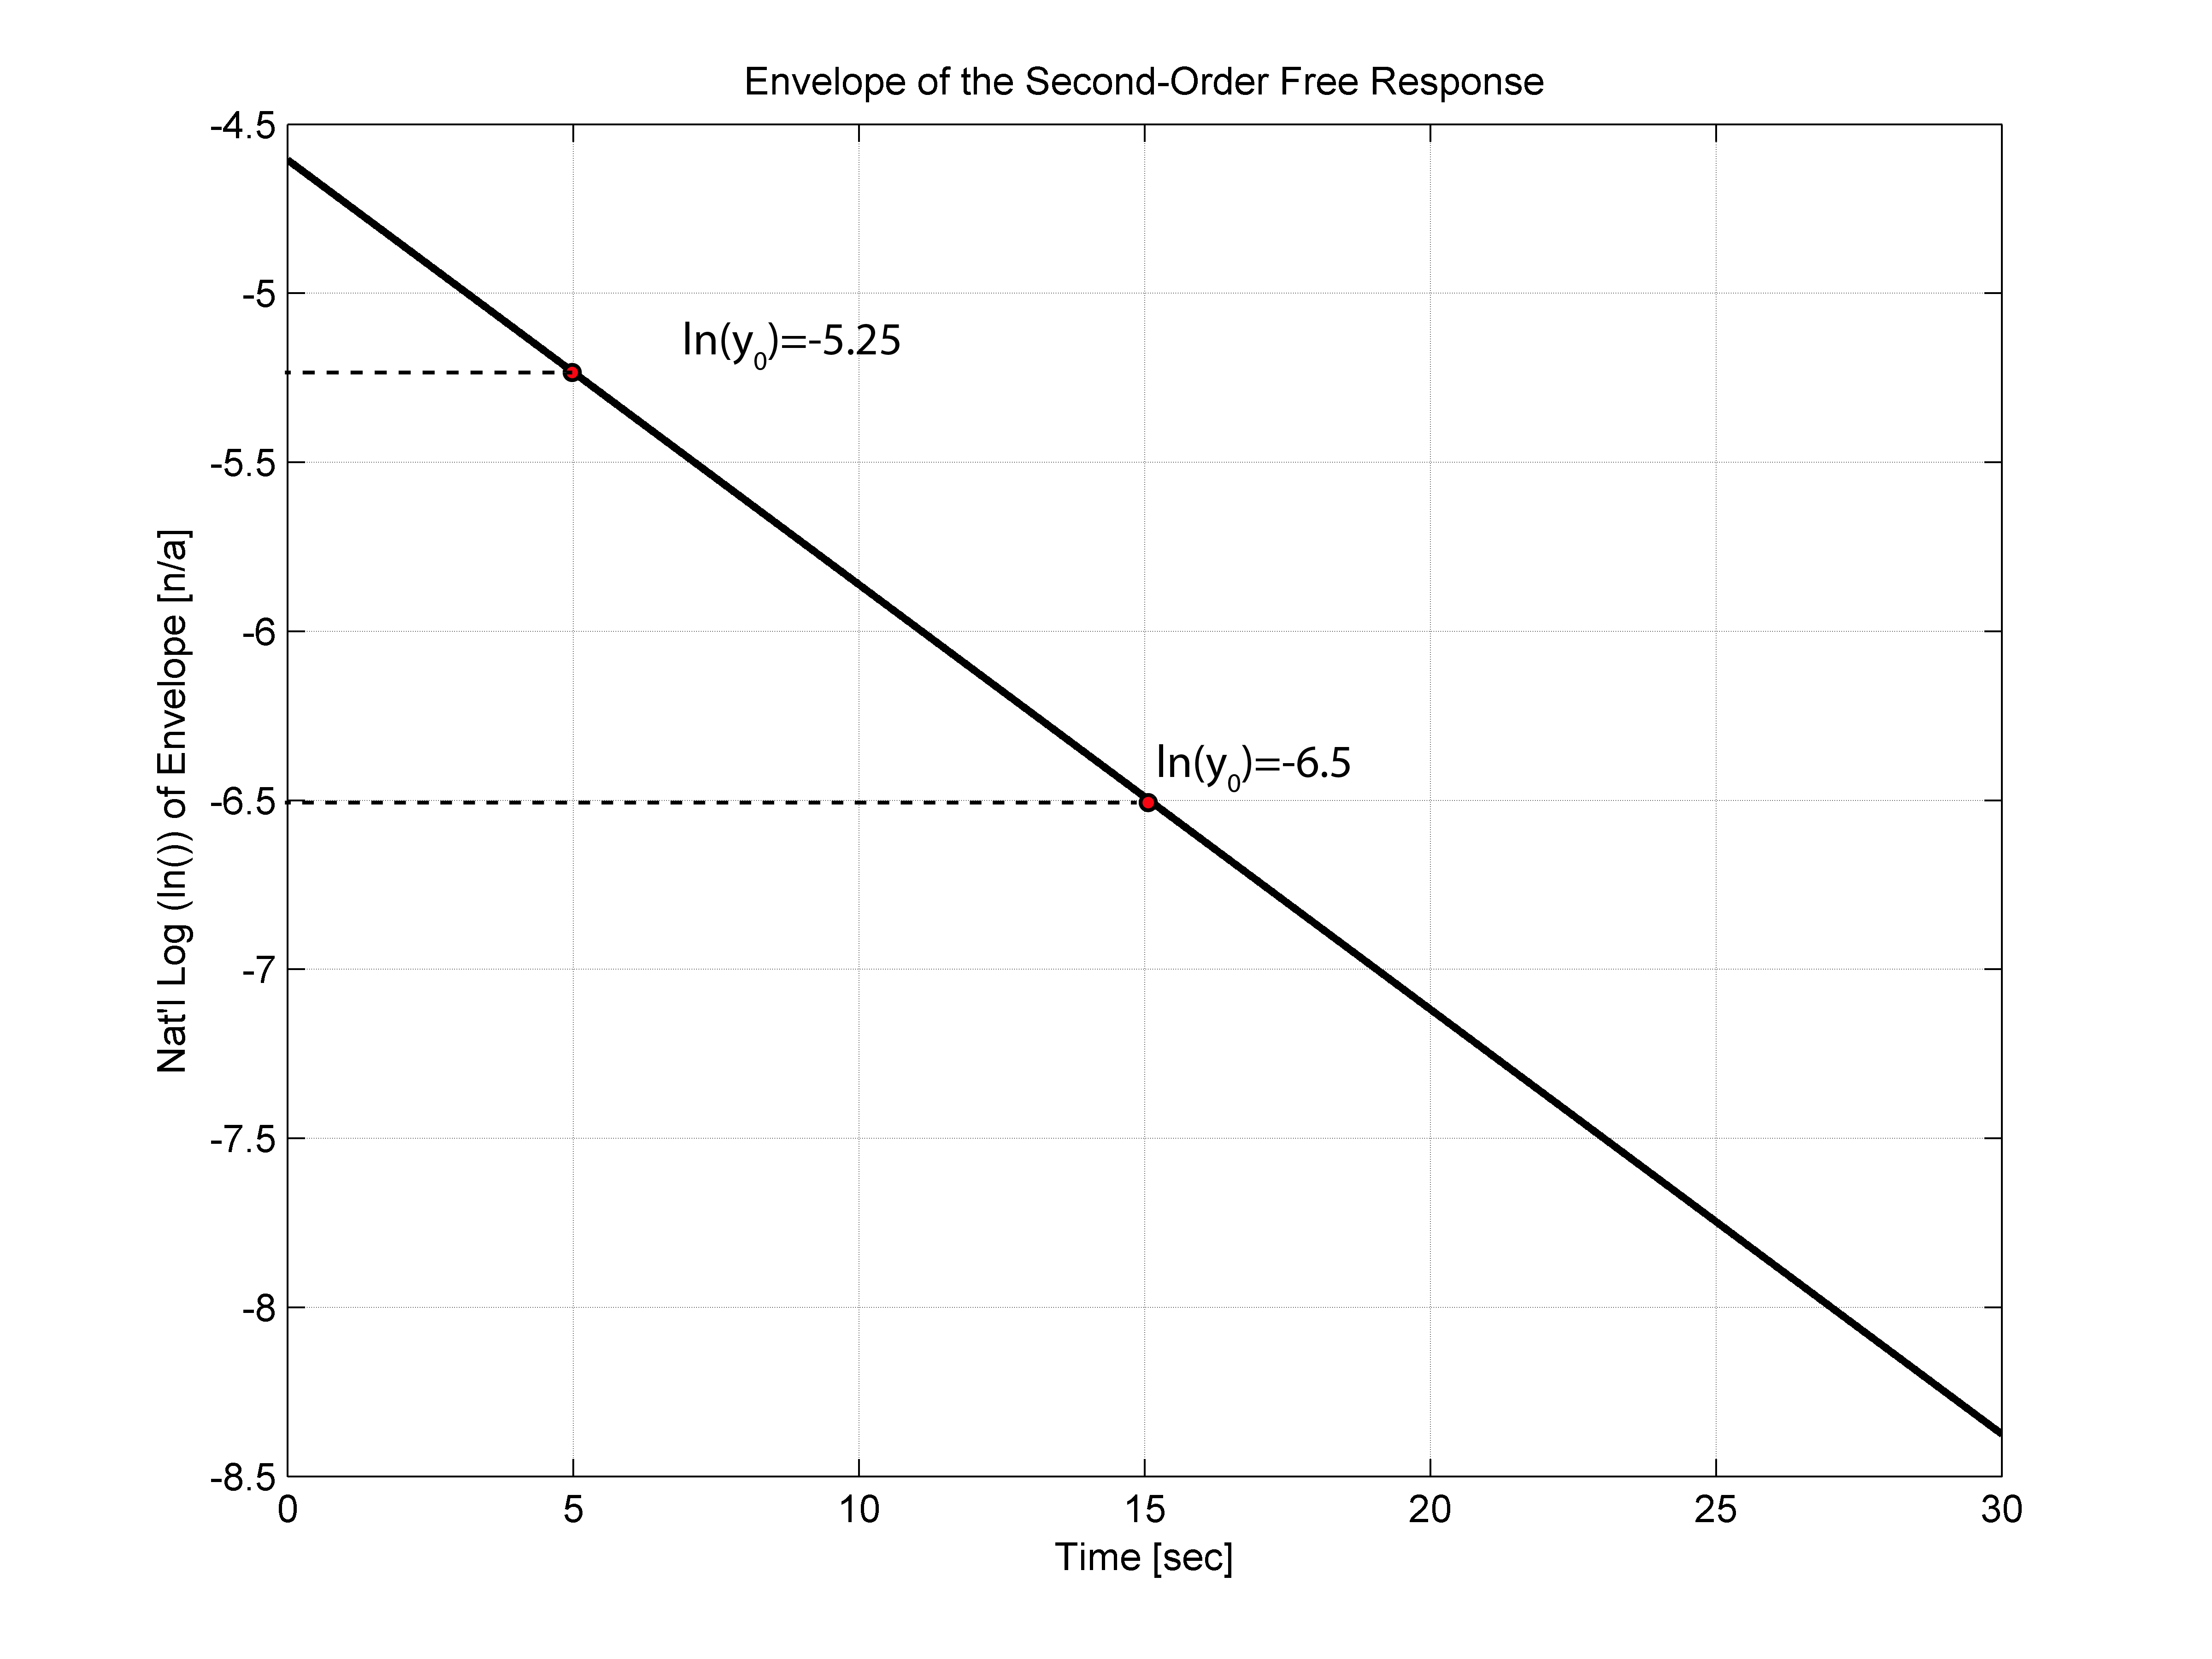
\includegraphics[width=0.6\textwidth]{second_order_env_ln_annote.png}}}
\caption{Plot of the exponential envelope shown in Figure~\ref{f:env}, but here the natural logarithm ($\ln()$) of the amplitude is plotted, i.e., $Y_{ln}$.}
\label{f:ln}
\end{figure}

Because we are using the second-order response model, we now just need to find the slope of the line in Figure~\ref{f:ln} and solve for the damping ratio.  The slope of the line can be expressed as
\begin{eqnarray}
m & = & \frac{\ln(y_0)-\ln(y_n)}{t_0-t_n}=-\zeta \omega_n \\
\label{e:slope} \\
m & = & \frac{\ln(y_0)-\ln(y_n)}{t_n-t_0}=\zeta \omega_n. \\
\label{e:slope2}
\end{eqnarray}
We can use (\ref{e:slope}) or (\ref{e:slope2} directly, but we have to deal with the fact that we don't know $\omega_n$.  It is important to note that the frequency of oscillation is the damped natural frequency ($\omega_d$) which is related to the undamped natural frequency by the relationship
\begin{equation}
\omega_d=\omega_n\sqrt{1-\zeta^2}.
\label{e:omegas}
\end{equation}
The logarithmic decrement method uses the peaks of the oscillating response to get around this trouble.  We know that the change in time is an integer number of periods of oscillation at the damped natural frequency
\begin{equation}
t_n-t_0 = \frac{n}{\omega_d / 2 \pi}.
\label{e:time}
\end{equation}
Now we can substitute (\ref{e:time}) and (\ref{e:omegas}) into (\ref{e:slope2}) to get
\[
\frac{\ln\left(\frac{y_0}{y_n}\right)}{n (2 \pi)} \omega_d = \zeta \omega_n
\]
and
\[
\frac{\ln\left(\frac{y_0}{y_n}\right)}{n (2 \pi)} \omega_n \sqrt{1-\zeta^2} = \zeta \omega_n.
\]
Next, let 
\[ \delta = \frac{1}{n}\ln\left(\frac{y_0}{y_n}\right) \]
and we solve for $\zeta$
\[
\zeta^2=\frac{\left(\frac{\delta}{2 \pi}\right)^2}{1+\left(\frac{\delta}{2 \pi}\right)^2}
\]
\[ \zeta = \frac{1}{\sqrt{1+\left(\frac{2\pi}{\delta}\right)^2}}. \]

It is interesting to consider that the logarithmic decrement method is doing this linear-fit with just two data points.  It would be interesting to do this linear fit with multiple data points using a least-squares approach to identify the damping ratio.  One advantage (along with a more precise result) is that you would be able to quantify the ``goodness-of-fit'' for the data using the correlation coefficient ($R^2$).





\printglossary[type=\thisgls]
\glsresetall

\chapter{Case Study: Strain and Acceleration of Cantilevered Beam} \label{c:accel}

In Chapter~\ref{c:strain} we examined the data acquisition system for measuring the static response of a cantilevered beam using a single strain gage.  In this chapter we'll consider adding an accelerometer to the tip of the beam to simultaneously measure the strain (at the root) and the acceleration (at the free-end) of the beam.  The DAQ system is illustrated in Figure~\ref{f:strainampdaq}.

\begin{figure}[hbt!]
\centering
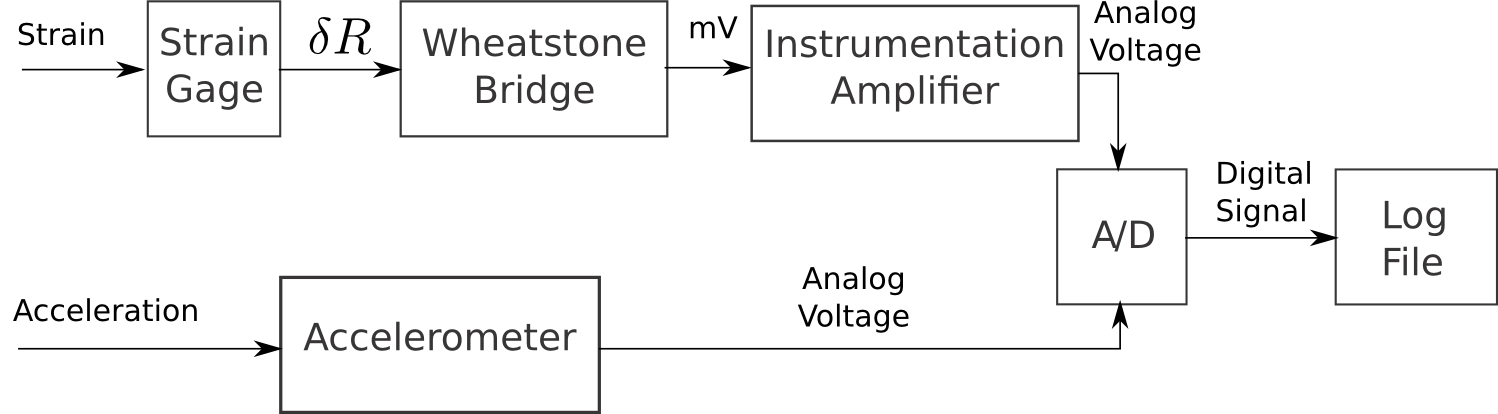
\includegraphics[width=\FigWidth\textwidth]{strain_amp_daq.png}
\caption{A data acquisition including strain gage and accelerometer.}
\label{f:strainampdaq}
\end{figure}

\section{Amplifying the Strain Signal}
Hopefully in Chapter~\ref{c:strain} you discovered that the output of a strain gage (with a Wheatstone bridge) is a small voltage---typically just a few millivolts.  This is a bit of a problem because a typical A/D operates with much larger input range: e.g., $\pm \unit[1.0]{V}$ or $\pm \unit[10.0]{V}$.  As we discussed in Chapter~\ref{c:daq}, the resolution of an A/D is finite, so using an A/D with a range much larger than the anticipate analog voltage input will have poor performance.

To improve the situation we can add an amplifier---the \emph{instrumentation amplifier} shown in Figure~\ref{f:strainampdaq}.  The gain of the amplifier ($K$) is constant multiplier so that the output voltage ($V_o$) is the product of the input voltage ($V_i$) and the gain, i.e.,
\[ V_o = K (V_i). \]

\begin{ex}
Ideally we would choose the gain of our amplifier such that the maximum anticipated voltage will be equivalent to the full-scale range setting of our A/D.  Consider the following strain gage scenario:
\begin{itemize}
\item Strain gage factor: $GF=2.0$
\item Wheatstone bridge excitation voltage: $V_s=\unit[9.0]{V}$
\item Maximum anticipated strain: $\epsilon=\unitfrac[0.001]{m}{m}$
\item A/D range: $E_{FSR}=\pm \unit[1.0]{V}$
\end{itemize}
What would be an appropriate gain setting for an amplifier that we would use in the DAQ system shown in Figure~\ref{f:strainampdaq}?
\end{ex}

\ifsolutions
\begin{soln}
First we need to predict the maximum voltage that we might anticipate from the Wheatstone bridge.  Using (\ref{e:gagebridge}
\[
V_o \approx V_s\left( \frac{(\mathrm{GF})\epsilon}{4} \right).
\]
and the parameters in the exercise we can anticipate the the maximum voltage output $V_o=\unit[4.5]{mV}$.  We would like to amplifiy this so that the output of the amplifier is equivalent to the full scale range (\unit[1]{V}).  A gain of 222.2 would give us exactly \unit[1]{V} of maximum output.
\end{soln}
\fi

\section{Accelerometer}
Unsurprisingly an accelerometer is a device for measuring acceleration.  Below are exercises to explore the application of a particular accelerometer to measuring the free response of a cantilevered beam.

\begin{ex}
Look-up the datasheet for the Analog Devices ADXL 335 accelerometer.  (The datasheet can be found online and is also available on the course website.)
\begin{itemize}
\item Read the section ``Theory of Operation''.  Write a few (1--2) sentences to summarize how the device measures acceleration.
\item Assuming a supply voltage of \unit[3]{V}...
  \begin{itemize}
  \item What is the maximum measurable acceleration: in g's and in \unit[]{m}{s$^2$}?
  \item What is the sensitivity of the accelerometer (with appropriate units)?
  \item (Hint: these quantities are listed in the ``Specifications'' section.)
  \end{itemize}
\end{itemize}
\end{ex}

\ifsolutions
\begin{soln}

\end{soln}
\fi



\begin{ex}
Given the cantilevered beam properties described in Exercise~\ref{ex:beamvib} and the free response of the model given in (\ref{e:damped}),
\begin{itemize}
\item What is the maximum acceleration at the free-end of the beam  you might anticipate for the free response of the system with the following initial conditions: $y(0)=\unit[10]{cm}$ and $\dot{y}(0)=0$? (Hint: you will need to differentiate the expression (\ref{e:secondfree}) and you can assume $\zeta=0$ and $\phi=0$. Check your units!)
\item Given this maximum acceleration and the sensitivity of the ADXL 335 from the previous exercise, what is the maximum voltage you should expect as output from an ADXL 335 mounted at the free-end of the beam?
\end{itemize}
\end{ex}

\ifsolutions
\begin{soln}
We need to differentiate twice the expression from (\ref{e:secondfree}) with $\zeta=0$ and $\phi=0$.  
\[
y(t) = C \left( \cos(\omega_n t ) \right)
\]
Using (\ref{e:C}) to evaluate the constant $C$ with these conditions we find that $C=y_o$, so...
\begin{eqnarray}
y(t) & = & y_o \left( \cos(\omega_n t ) \right) \\
\dot{y}(t) & = & y_o * \omega_n \left(-\sin(\omega_n t ) \right) \\
\ddot{y}(t) & = & y_o * \omega_n^2 \left( -\cos(\omega_n t ) \right) \\
\ddot{y}(t) & = & \unit[10]{cm} (\unitfrac[32.6]{rad}{s})^2 \left( -\cos(\omega_n t ) \right) \\
\ddot{y}(t) & = & \unit[10]{cm} (\unitfrac[32.6]{rad}{s})^2 \left( -\cos(\omega_n t ) \right) \\
\ddot{y}(t) & = & \unitfrac[106]{m}{s^2} \left( -\cos(\omega_n t ) \right) \\
\ddot{y}(t) & = & \unit[10.8]{g} \left( -\cos(\omega_n t ) \right) 
\end{eqnarray}
So the amplitude of the acceleration is \unit[10.8]{g}.  The sensitivity of the ADXL 335 is \unit[300]{mV}{g} which indicates that the maximum output from the accelerometer is $10.8*300 = \unit[3240]{mV} = \unit[3.24]{V}$. However, the maximum acceleration the device can sense is $\pm\unit[3]{g}$, so we should probably start with an initial displacement of less than \unit[10]{cm}!
\end{soln}
\fi





%\bibliographystyle{../latexlib/latex_ieee/IEEEtran}
%\bibliography{../bibtex/ref_bbing_master}


% that's all folks
% that's all folks
\end{document}


